\documentclass[fr]{../../../eplsummary}

\usepackage{siunitx}  %symbole angstrom
\usepackage{titlesec} %Modifier la taille des titres
\titleformat*{\section}{\LARGE\bfseries}
\titleformat*{\subsection}{\Large\bfseries}
\titleformat*{\subsubsection}{\large\bfseries}

\numberwithin{equation}{section} %Numéroter les équations par section
\numberwithin{figure}{section}   %Numéroter les figures par section
\setlength{\parindent}{0pt} %Modifier l'alinéa des paragraphes

\expandafter\def\expandafter\normalsize\expandafter{%
	\normalsize
	\setlength\abovedisplayskip{20pt}
	\setlength\belowdisplayskip{20pt}
	\setlength\abovedisplayshortskip{20pt}
	\setlength\belowdisplayshortskip{20pt}
}

\usepackage{tikz}
\usetikzlibrary{babel, scopes, arrows.meta, calc, decorations.pathmorphing, decorations.markings, shapes.geometric}
\usepackage{pgfplots}

%\Star[opt]{r1}{r2}{pos}
\newcommand\Star[4][]{%
\path[#1]  #4 +(0:#2) -- +(45:#3) -- +(90:#2) -- +(135:#3) -- +(180:#2) -- +(225:#3) -- +(270:#2) -- +(315:#3) -- cycle;}

%polstar[opt]{radius}{position}
\newcommand{\polstar}[3][]{
\Star[fill=black,#1]{1*#2}{0.28*#2}{#3}
\Star[#1, fill=white]{0.8*#2}{0.08*#2}{#3}
}
% Syntax: \centerarc[draw options] (x,y) (r, a1, a2) !spaces are important!
\def \centerarc[#1] (#2) (#3,#4,#5)
{\draw[#1] (#2) + ({#3*cos(#4)},{#3*sin(#4)}) arc (#4:#5:#3);}

%\base[options]{texte après}
\newcommand{\base}[2][]{
\draw (0,0) node {\tiny{$\bullet$}};
\draw [thick, .-latex, #1] (0,0) -- (2,0) node[below]{$\vec{e_{x}}$#2};
\draw [thick, .-latex, #1] (0,0) -- (0,2) node[right]{$\vec{e_{y}}$#2};
}

%\bigarrow[options]{scale}{x}{y}
\newcommand{\bigarrow}[4][]{
  \draw [#1] (#3,#4+0.35*#2)-|(1.2*#2+#3,#4+#2)--(2.5*#2+#3,#4+0)--(1.2*#2+#3,#4-#2)|-(#3,#4-0.35*#2)--cycle;
}

\definecolor{dgreen}{RGB}{0,150,0}
\definecolor{lblue}{RGB}{100,100,255}

%\eye[opt]{size}{x}{y}{rotation}
\newcommand{\eye}[5][]% size, x, y, rotation
{   \draw[rotate around={#5:(#3,#4)}, #1] (#3,#4) -- ++(-.5*55:#2) (#3,#4) -- ++(.5*55:#2);
    \draw[#1] (#3,#4) ++(#5+40:.75*#2) arc (#5+40:#5-40:.75*#2);
    % IRIS
    \draw[fill=blue] (#3,#4) ++(#5+55/3:.75*#2) arc (#5+180-55:#5+180+55:.28*#2);
    %PUPIL, a filled arc
    \draw[fill=black] (#3,#4) ++(#5+55/3:.75*#2) arc (#5+55/3:#5-55/3:.75*#2);
}

%\rgb{r}{g}{b} (de 0 à 255)
\newcommand{\rgb}[3]{rgb,255:red,#1; green,#2; blue,#3}

%\tbase[options]{xi}{additional text}
\newcommand{\tbase}[3][]{
\draw [thick, .-latex, #1] (0,0) -- ({2*(cosh(#2)}, {2*sinh(#2))}) node[below]{$\vec{e_{x}}$#3};
\draw [thick, .-latex, #1] (0,0) -- ({2*(sinh(#2)}, {2*cosh(#2))}) node[right]{$\vec{e_{y}}$#3};
}


\newcommand{\eq}{\; = \;}
\newcommand{\eqq}{\quad = \quad}
\newcommand{\cRM}[1]{\MakeUppercase{\romannumeral #1}}  % Capital
\newcommand{\approxtext}[1]{\ensuremath{\stackrel{\text{#1}}{\approx}}}
\newcommand{\p}{\partial}

\newcommand{\ch}{\mathrm{ch}}
\newcommand{\sh}{\mathrm{sh}}
\let\oldth\th % la commande
\renewcommand\th{\mathrm{th}}

\newcommand{\pfpart}[2]{\left(\fpart{#1}{#2}\right)} %équivalent à (\fpart{}{}) --> parenthèses bien dimentionnées

\hypertitle{Relativité restreinte}{4}{PHYS}{1231}
{Valentin Fonck \and Pierre Laboureur \and Miguel De Le Court}
{Jean-Marc Gérard (PHYS)}

\newpage
%%%%%%%%%%%%%%%%%%%%%%%%%%%%%%%%%%%%%%%%%%%%%%




\newpage

\section{Approche géométrique}
Il sera ici question d'introduire géométriquement certaines équations et concepts qui seront développés tout au long du cours.

\subsection{Pythagore pour mesurer des distances}

Considérons un chemin quelconque \textbf{linéaire} dans un repère cartésien muni de deux axes: x et y. Le repère cartésien correspond donc à un espace vectoriel engendré par la base: $<\vec{e_{x}},\vec{e_{y}}>$. Le théorème de Pythagore permet de calculer la distance au carré $\Delta l^2$ entre le point de départ et le point d'arrivée de notre chemin. \footnote{A noter que $\Delta l^2$ équivaut bien à $(l_2 - l_1)^2$ et non $(l_2^2 - l_1^2)$. Cette remarque reste valable tout au long du document.}
\begin{equation}
	\Delta l^2 = \Delta x^2 + \Delta y^2
	\label{pyth}
\end{equation}
Cette équation bien que triviale repose sur l'hypothèse d'un espace euclidien. La pierre angulaire de la suite du raisonnement sera de considérer les cas où cette hypothèse n'est pas vérifiée.

\subsection{Notion de métrique}

Dans le cas d'une trajectoire non-linéaire (une courbe dans le plan ou une trajectoire quelconque dans un espace courbe par exemple), la distance parcourue peut se calculer en sommant des trajectoires linéaires infinitésimales. Une approche intuitive de la métrique est de la considérer comme un opérateur linéaire (donc représentable par une matrice) multipliant deux vecteurs (produit scalaire).

Le théorème de Pythagore \eqref{pyth} peut ainsi se réécrire, pour des trajectoires infinitésimales comme suivant.
\begin{equation}
	dl^2 = \sum_i dx_i^2 = \delta_{ij} \; dx^i \; dx^j \quad \text{avec} \quad    \delta_{ij} = \left\{
	\begin{array}{ll}
		1   \quad \forall \; i = j \\
		0   \quad \forall \; i \ne j
	\end{array}
	\right.
	\label{metr}
\end{equation}
A noter que la \textbf{convention d'Einstein} est ici utilisée: lorsqu'un indice est répété deux fois, une fois en bas (indice) et une fois en haut (exposant), c'est équivalent à sommer sur cet indice. Par conséquent, l'équation \eqref{metr} peut être réécrite comme suivant, avec $d$ le nombre de dimensions.\footnote{On retombe effectivement sur Pythagore dans le cas où d=2...essayez ;)}
\begin{equation}
	dl^2 = \sum_{i=1}^{d} \sum_{j=1}^{d} \quad \delta_{ij} \; dx_i \; dx_j
\end{equation}
Nous adopterons la convention d'Einstein plus tard dans ce document, parce qu'elle est nettement plus aisée avec le formalisme tensoriel.
L'opérateur $\delta_{ij}$ peut également s'écrire sous la forme d'une matrice 2D:
\begin{equation}
\delta_{ij} =
	\begin{pmatrix}
		1 & 0 \\
		0 & 1
	\end{pmatrix}
\end{equation}
Cette matrice est appelée \textbf{métrique de l'espace}. Il existe une infinité de variations de cette matrice qui conservent les propriétés de l'espace. Par exemple, le passage en coordonnées polaire n'affecte pas les résultats obtenus dans les coordonnées cartésiennes.
\begin{equation}
	g_{ij} = \begin{pmatrix}
	1 & 0\\
	0 & r^2
	\end{pmatrix}
	\end{equation}
	\begin{equation}
	dl^2 \eq dr^2 + r^2 d\theta^2 \eq g_{ij} \; dx_i \; dx_j
\end{equation}
Il est intéressant de noter que la métrique peut tout à fait dépendre des coordonnées, autrement dit de la position dans l'espace (via le $r$ dans l'exemple). De plus, un changement de la forme de la métrique $g_{ij}$ ne signifie pas forcément un changement d'espace: la métrique correspond simplement à une autre base du même espace euclidien ou a un autre système de coordonnées (ici les coordonnées polaires). L'espace en lui-même par contre ne change pas (deux points seront tonjours séparés par la même distance par exemple).

\newpage

\subsection{Rotations}

Supposons que l'on souhaite effectuer une rotation d'un angle $\theta$ sur les vecteurs $<\vec{e_{x}},\vec{e_{y}}>$, comme représenté à la figure \eqref{rot1}. Nommons $<\vec{e'_{x}},\vec{e'_{y}}>$ la nouvelle base obtenue.
\begin{figure}[!ht]
	\centering
	%base
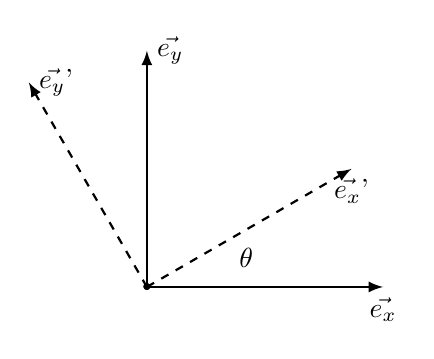
\begin{tikzpicture}[scale=1.5]
  %\node [black] at (0,0) {\Large{.}};
  \base[]{}
  \centerarc[thick, -latex] (0,0) (0.7,0,30)
  \centerarc[thick, -latex] (0,0)  (0.7,90,120)
  \node [right] at (0.7,0.25) {$\theta$};
  \begin{scope}[rotate=30]
    \base[dashed]{'}
  \end{scope}

  %\draw [#1](a.#4) arc (#4:{#4+#5}:#3);
  %\draw [thick, .-latex] (0,0)  arc (90:200:1);
\end{tikzpicture}

	\caption{Schéma du changement de base}
	\label{rot1}
\end{figure}\\
On peut donc écrire le changement de base:
\begin{equation}
	\begin{pmatrix}
		\vec{e'_{x}} \\
		\vec{e'_{y}}
	\end{pmatrix}
		\eq
		R
		\begin{pmatrix}
			\vec{e_{x}} \\
			\vec{e_{y}}
		\end{pmatrix}
		\quad \textrm{avec} \quad
	R \eq \begin{pmatrix}
			\cos(\theta) & -\sin(\theta) \\
			\sin(\theta) & \cos(\theta)
		\end{pmatrix}
	\label{ortho1}
\end{equation}
L'orthogonalité des vecteurs de la nouvelle base $<\vec{e'_{x}},\vec{e'_{y}}>$ peut s'exprimer par le produit matriciel suivant:
\begin{equation}
		\begin{pmatrix}
		\vec{e'_{x}} \\
		\vec{e'_{y}}
	\end{pmatrix} \cdot    \begin{pmatrix}
		\vec{e'_{x}}
		\vec{e'_{y}}
	\end{pmatrix}
	\eq    \begin{pmatrix}
	 1 & 0 \\
	 0 & 1
	 \label{ortho2}
\end{pmatrix}
\end{equation}
En combinant les équations \eqref{ortho1} et \eqref{ortho2}:
\begin{equation}
	R \cdot     \begin{pmatrix}

		\vec{e_{x}} \\
		\vec{e_{y}}

	\end{pmatrix}
	\cdot
		\begin{pmatrix}

		\vec{e_{x}}
		\vec{e_{y}}

	\end{pmatrix}
	\cdot
	R^T
	\eq
	I
	\; \overset{\Delta}{\eq} \; \textrm{Matrice identité}
\end{equation}
La base initiale étant déjà orthogonale:
\begin{equation}
	R\cdot R^T = I
\end{equation}
Il est ainsi démontré que l'inverse de la matrice de rotation $R(\theta)$ est $R(-\theta)$. Cela se vérifie en utilisant l'expression \eqref{ortho1}.
\begin{equation}
	R^{-1}(\theta) = R(-\theta)
	\label{propriete}
\end{equation}
En effet, effectuer une rotation d'un angle puis de son opposé revient à l'opération identité. De plus, puisque deux rotations consécutives se traduisent par le produit de deux matrices de rotations, si on multiplie $R(\theta)$ avec $R(-\theta)$, on obtient bien la matrice identité.

\subsection{Pseudo-rotations}

Il s'agit ici d'appliquer le même traitement au temps (qui n'est finalement qu'une dimension comme une autre) qu'aux dimensions classiques d'espace. Il faut donc trouver un outil mathématique semblable à la matrice de rotation. Seulement, un problème se pose directement: le temps n'est pas cyclique mais s'écoule inexorablement. Il est ainsi impossible d'utiliser des fonctions trigonométriques en raison de leur nature cycliques. On se propose donc d'utiliser les fonctions hyperboliques correspondantes.\footnote{Ceci prendra sens dans la suite du document}\\
C'est pourquoi $L(\xi)$, le petit cousin hyperbolique de $R(\theta)$, doit être définit.
\begin{equation}
	L(\xi) = \begin{pmatrix}
		\cosh(\xi) & \sinh(\xi) \\
		\sinh(\xi) & \cosh(\xi)
	\end{pmatrix}
\end{equation}
A l'instar de $R(\theta)$, $L(\xi)$ possède la propriété \eqref{propriete}:
\begin{equation}
L^{-1}(\xi) = L(-\xi)
\end{equation}
Pour conserver l'orthogonalité de la base, il faut supposer une matrice A telle que:
\begin{equation}
	L(\xi) \cdot A \cdot L^T(\xi) = A
\end{equation}
En se rappelant que $\cosh^2(\xi) - \sinh^2(\xi) = 1$, la nouvelle métrique est trouvée:
\begin{equation}
	A = \begin{pmatrix}
		1 & 0 \\
		0 & -1
	\end{pmatrix}
\end{equation}
 %utile de placer le schéma d'une pseudo-rotation



\subsection{Lien avec la mécanique de Newton}

Était-ce une bonne idée de remplacer les rotations de l'espace ou tout autre transformation par les pseudo-rotations dans l'espace-temps? La réponse à cette question n'est oui qu'à condition de retrouver une transformation connue dans une certaine limite dite classique. Pour ce faire, il est nécessaire de reprendre les fondement de la mécanique newtonienne au travers des transformations galiléennes:
\begin{equation}
	\left\{
	\begin{array}{ll}
		t' = t \\
		\vec{x'} = \vec{x} + \vec{v_0} \cdot t
	\end{array}
	\right.
\end{equation}
Afin de comparer les transformations galliléennes à la transformation créée ci-haut, il est nécessaire que les composantes des vecteurs à comparer soient de même dimension (càd aient les mêmes unités). Dès lors, la dimension temporelle doit être multipliée par  une constante $c$ (pour l'instant non-déterminée) ayant les dimensions d'une vitesse. \footnote{Il aurait été équivalent de diviser les dimensions spatiales par $c$, mais ce n'est qu'un choix de convention.} Pour cette partie le réferentiel $\mathcal{R'}$ sera <<au repos>> et le réferentiel $\mathcal{R}$ se déplace dans $\mathcal{R'}$ à une vitesse $v_0$ dans la direction $x$ (voir figure \ref{refGalilBase}).
\begin{equation}
	\begin{pmatrix}
		c \cdot t' \\
		x'
	\end{pmatrix}
	\stackrel{?}{=}
	L(\xi) \cdot
	\begin{pmatrix}
		c \cdot t \\
		x
	\end{pmatrix}
\end{equation}

\begin{figure}[!ht]
		\centering
		\begin{tikzpicture}
  \begin{scope}[shift={(-3,0)}]
    \draw (0,0) node {\tiny{$\bullet$}};
    \draw [thick, latex-latex] (0,2) node[right] {$ct'$} -- (0,0) -- (2,0) node[below] {$x'$};
    \node[above] at (1.2,2.1) {$\mathcal{R'}$};
  \end{scope}

  \begin{scope}[shift={(3,0)}]
    \draw (0,0) node {\tiny{$\bullet$}};
    \draw [thick, latex-latex] (0,2) node[right] {$ct$} -- (0,0) -- (2,0) node[below] {$x$};
    \node[above] at (1.2,2.1) {$\mathcal{R}$};
    \draw[-latex, ultra thick, red] (1.2,1.1)++(-0.7,0)--++(1.5,0) node[right] {$\vec{v_0}$};
  \end{scope}
\end{tikzpicture}

		\caption{Schéma des réferentiels galliléens}
		\label{refGalilBase}
\end{figure}

Dans le cas où $\xi \approx v_0 / c\approx 0$, il est possible d'approximer les fonctions hyperboliques comme $\cosh(\xi) \approx 1$ et $\sinh(\xi) \approx \xi$, ce qui permet de retrouver les transformations galliléennes\footnote{Le fait de retomber sur les transformations galliléennes est nécessaire: la théorie précédente n'est pas détruite mais améliorée.}:
\begin{equation}
	\left\{
	\begin{array}{ll}
		c \cdot t' &= \quad  \cosh(\xi) \cdot ct + \sinh(\xi) \cdot x \quad \approx \quad ct + \dfrac{v_0}{c} x \quad \approx \quad c \cdot t
		\\[7pt]
		x'    &= \quad  \sinh(\xi) \cdot ct + \cosh(\xi) \cdot x  \quad \approx \quad \dfrac{v_0}{c} \cdot ct + x \eqq v_0 \cdot t + x
	\end{array}
	\right.
\end{equation}

\subsection{Conséquences pour le référentiel}

En effectuant le produit matriciel de la base $<\vec{e_x},\vec{e_y}>$ par la matrice de pseudo-rotation $L(\xi)$, la nouvelle base $<\vec{e'_{x}},\vec{e'_{y}}>$ est exprimée.
\begin{equation}
	\begin{pmatrix}
		\vec{e'_{x}}    \\     \vec{e'_{y}}
	\end{pmatrix}
	\eq
	L(\xi) \cdot
	\begin{pmatrix}
		\vec{e_{x}}     \\    \vec{e_{y}}
	\end{pmatrix}
	\eq
	\begin{pmatrix}
		\cosh(\xi) \; \vec{e_x} + \sinh(\xi) \; \vec{e_y}\\
		\sinh(\xi) \; \vec{e_x} + \cosh(\xi) \; \vec{e_y}
	\end{pmatrix}
	\label{chgmt}
\end{equation}
En approximant les fonction hyperboliques comme $\cosh(\xi) \approx 1$ et $\sinh(\xi) \approx \xi$ pour $\xi \approx 0$, la nouvelle base devient:
\begin{equation}
	\begin{pmatrix}
	\vec{e'_{x}}\\
	\vec{e'_{y}}
	\end{pmatrix} =
	\begin{pmatrix}
	\vec{e_x} + \xi \vec{e_y}\\
	\xi\vec{e_x} + \vec{e_y}
	\end{pmatrix}
\end{equation}
Les vecteurs, initialement perpendiculaires, vont donc progressivement devenir des combinaisons linéaires l'un de l'autre. La figure \eqref{pseudorot} permet d'observer que les deux vecteurs de la base tendent à se confondre quand la vitesse $v_0$ d'un objet s'approche de la vitesse $c$ ($\xi = v_0 / c \rightarrow 1$). En identifiant c comme la vitesse de la lumière, on observe que l'espace se confond avec le temps quand on s'approche de la vitesse de la lumière!
\begin{figure}[!ht]
		\centering
		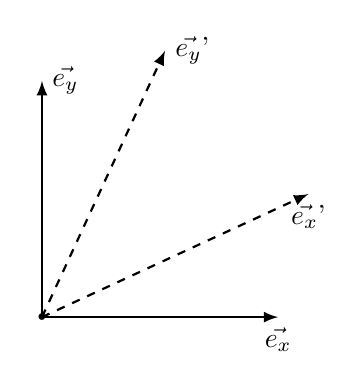
\begin{tikzpicture}[scale=1.5]
  \base{}
  \tbase[dashed]{0.5}{'}
\end{tikzpicture}

		\caption{Schéma du changement de base}
		\label{pseudorot}
\end{figure}

\newpage

\subsection{Justification pour la valeur attribuée à $\xi$}

Le changement de base \eqref{chgmt} peut être noté pour des distances et temps infinitésimaux:
\begin{equation}
	 \begin{pmatrix}
		cdt'\\
		dx'
	\end{pmatrix}
	\eq
	\begin{pmatrix}
		\cosh(\xi) & \sinh(\xi) \\
		\sinh(\xi) & \cosh(\xi)
	\end{pmatrix}
	\begin{pmatrix}
		c dt\\
		x
	\end{pmatrix}
	\label{chgmtBase}
\end{equation}
Pour un référentiel immobile ($dx' = 0$), un système de deux équations est obtenu. En divisant ces deux équation, une expression de $\xi$ est obtenue.
\begin{equation}
	\left\{
	\begin{array}{ll}
		c \cdot dt \eq \quad \cosh(\xi) \cdot c \cdot dt'
		\\
		dx   \quad \eq \quad \sinh(\xi) \cdot c \cdot dt'
	\end{array}
	\right.
	\quad \Rightarrow \quad
	\tanh(\xi)=\dfrac{ dx}{c\cdot dt} = \dfrac{v_0}{c}
\end{equation}
Pour $\xi << 1$ on peut donc écrire:
\[
	\xi = \dfrac{v_0}{c}
\]
En identifiant $c$ comme la vitesse de la lumière, on constate qu'il est impossible de dépasser la vitesse de la lumière car $\abs{\tanh(\xi)} < 1 \quad \forall \xi \in \mathbb{R}$. Ainsi, la vitesse universelle $c$ borne $v_0$ : $-c < v_0 < c$.
\begin{figure}[!ht]
	\centering
	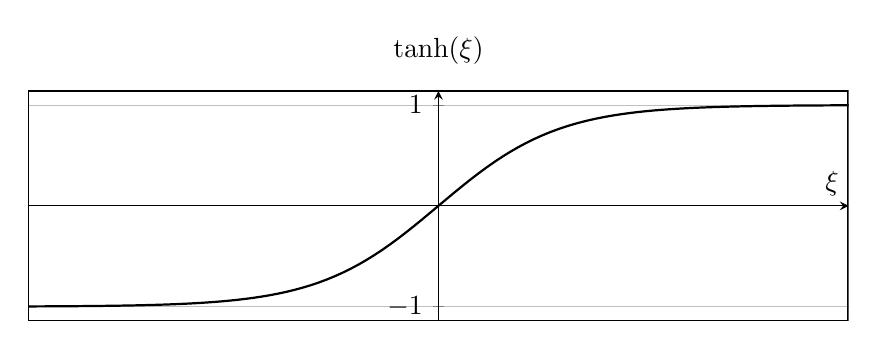
\begin{tikzpicture}
  \begin{axis}[
      samples=121,
      xmin=-3,
      xmax=3,
      ymin=-1,
      ymax=1,
      width=12cm,
      height=4.5cm,
      disabledatascaling,
      grid=both,
      %font=\footnotesize,
      %grid style={line width=.1pt, draw=red},
      %major grid style={line width=.2pt,draw=gray!50},
      %minor tick num=1,
      axis lines=middle,enlargelimits=0.07,
      %execute at begin axis={
      execute at end axis={        \draw[thick] (rel axis cs:0,0) -- (rel axis cs:1,0) -- (rel axis cs:1,1) -- (rel axis cs:0,1) --cycle;},
      %xticklabels={},
      %yticklabels={},
      xtick={-10,0,10},
      ytick={-10,-9,...,10},
      %ylabel={$\tanh(\xi)$},
      xlabel={$\xi$},
      title={$\tanh(\xi)$},
      %legend pos=south east,
    ]

    \addplot [thick, domain=-4:4] ({x}, {tanh(x)});
    %\node[anchor=south,rotate=90] at (0,-.2) {$\xi$};
  \end{axis}
\end{tikzpicture}

\end{figure}\\
Il est également possible de retrouver une relation permettant de trouver les valeurs des fonctions hyperboliques:
\[
	\cosh^2(\xi) - \sinh^2(\xi) \eq 1
		\quad \Leftrightarrow \quad
	1 - \tanh^2(\xi) \eq \dfrac{1}{\cosh^2(\xi)}
		\quad \Leftrightarrow \quad
	\cosh^2(\xi) \eq \dfrac{1}{1 - \tanh^2(\xi)}
\]
En réécrivant l'équation \eqref{chgmtBase} avec les valeurs des fonction hyperboliques, il est possible de dériver les \textbf{transformations de Lorentz}:
\begin{equation}
	\left\{
	\begin{array}{ll}
		\cosh(\xi) \eq \dfrac{1}{\sqrt{1 - v_0^2/c^2}} \overset{\Delta}{\eq} \gamma
		\\[14pt]
		\sinh(\xi) \eq \dfrac{v_0/c}{\sqrt{1 - v_0^2/c^2}} \overset{\Delta}{\eq} \beta\gamma
	\end{array}
	\right.
		\quad \Rightarrow \quad
	\boxed{
		\begin{pmatrix}
			cdt'\\
			dx'
		\end{pmatrix}
			\eq \gamma \cdot
		\begin{pmatrix}
			1 & \beta \\
			\beta & 1
		\end{pmatrix}
		\begin{pmatrix}
			c dt\\
			x
		\end{pmatrix}
	}
\end{equation}
\newpage

\section{Lumière... et action!}
\subsection{L'éther}

	Jusqu'au 19$^{\textrm{ème}}$, les physiciens affirmaient que la lumière se déplaçait dans une substance nommée éther. Cette affirmation vient d'une extrapolation: le son nécessitant un support pour se propager (air, eau, etc.), il est légitime de penser que la lumière, également une onde, dispose de son propre support: l'éther.

	Michelson réfuta cette idée en utilisant un interféromètre: voulant au départ déterminer les propriétés de l'éther, il se retrouve avec un résultat réfutant l'existence de l'éther.

\subsection{Interféromètre de Michelson}

	Supposons l'existence de l'éther, une substance dans laquelle baigne tout objet et dans laquelle un objet émettant de la lumière est source d'ondulations. Un observateur (appelons-le Gregory) devrait observer des vitesses différentes de la lumière en fonction de son déplacement dans l'éther ($\approx$ effet Doppler). Pour visualiser et quantifier cela, changeons de décor en plaçant Gregory dans une rivière.

	\subsubsection{Temps de parcours dans l'eau}

		Considérons une rivière de largeur L et forçons Gregory à nager dedans. Nommons $c$ la vitesse de Gregory dans l'eau quand il n'y a pas de courant et v$_0$ la vitesse du courant.

		Nous pouvons observer deux temps de parcours distincts en imposant à Gregory deux chemins différents mais de même longueur:
		\begin{itemize}
			\item Parcours A: un aller-retour \textbf{perpendiculaire} à la direction du courant et de longueur totale 2L
			\item Parcours B: un aller-retour \textbf{parallèle} à la direction du courant et de longueur totale 2L
		\end{itemize}
		\begin{figure}[!ht]
			\centering
			
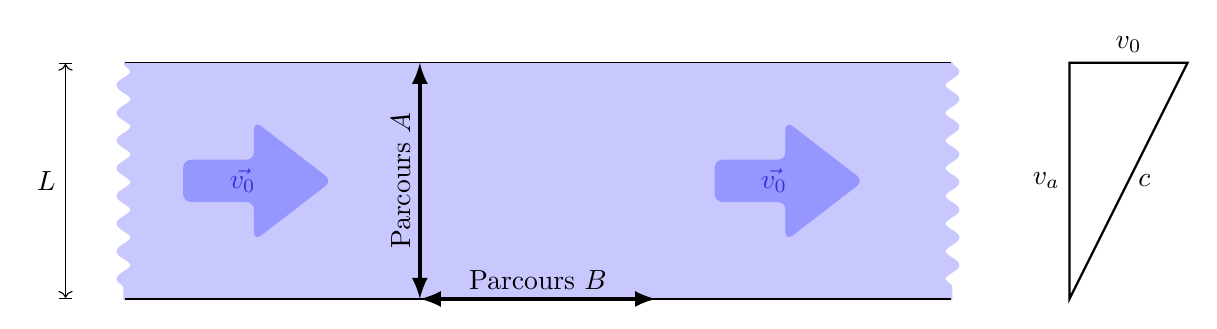
\begin{tikzpicture}[scale=0.75]
  %eau de la rivière
  \draw [thick, fill=\rgb{200}{200}{255}, color=\rgb{200}{200}{255}] decorate [decoration={snake}] {(14,4) -- (14,0)} -- (0,4) decorate [decoration={snake}] {(0,4) -- (0,0)} -- (14,0);
  \path [fill=\rgb{200}{200}{255}] (0.2,0) -- (13.8,0) -- (13.8,4) -- (0.2,4);
  %grosses flèches
  \bigarrow[color=\rgb{150}{150}{255}, fill=\rgb{150}{150}{255}, rounded corners=1mm]{1}{1}{2}
  \draw [color=\rgb{50}{50}{210}] node at (2,2) {$\vec{v_0}$};

  \bigarrow[color=\rgb{150}{150}{255}, fill=\rgb{150}{150}{255}, rounded corners=1mm]{1}{10}{2}
  \draw [color=\rgb{50}{50}{210}] node at (11,2) {$\vec{v_0}$};

  %les berges noires
  \draw (0,0) -- (14,0);
  \draw (0,4) -- (14,4);

  %double flehce cotation evec le "L"
  \draw [|<->|] (-1,0) -- (-1,4);
  \draw node [left] at (-1,2) {$L$};

  %flèches des parcours
  \draw [latex-latex, ultra thick, black] (5,0) -- (5,4);
  \draw [latex-latex, ultra thick, color=\rgb{0}{0}{0}] (5,0) -- (9,0);

  %labels des parcours
  \draw node [rotate=90, left, anchor=south, black] at (5,2) {Parcours $A$};
  \draw node [above, color=\rgb{0}{0}{0}] at (7,0) {Parcours $B$};

  %triangle à droite
  \draw [thick] (16,0) |- (18,4) --cycle;
  \draw node [above] at (17,4) {$v_0$};
  \draw node [left] at (16,2) {$v_a$};
  \draw node [right] at (17,2) {$c$};
\end{tikzpicture}

			\caption{Schéma de la rivière de Gregory}
			\label{gregory}
		\end{figure}
		Il est ainsi possible de calculer le temps de parcours de Gregory pour chacun des deux trajets. Lorsque deux vitesses influent Gregory (càd sa propre vitesse $c$ et la vitesse du courant v$_0$), il faut effectuer un addition \textbf{vectorielle} et prendre la norme du vecteur résultant. Par exemple, la vitesse v$_a$ s'exprime grâce à l'utilisation de Pythagore dans le triangle adjacent à la figure \eqref{gregory}. Les temps de parcours de deux chemins sont ainsi obtenus:
		\begin{equation}
			\left\{
			\begin{array}{ll}
				\Delta t_{A} \eqq \dfrac{L}{v_a} + \dfrac{L}{v_a}
							 \eqq \dfrac{2L}{\sqrt{ c^2 - v_0^2  }}
				\\[15pt]
				\Delta t_{B} \eqq \dfrac{L}{c+v_0} + \dfrac{L}{c-v_0}
							 \eqq \dfrac{2cL}{c^2 - v_0^2}
			\end{array}
			\right.
		\end{equation}
		La différence entre les temps de parcours peut ainsi être aisément calculée:
		\begin{equation}
			\Delta t_{BA} = \Delta t_{B} - \Delta t_{A}
							= \dfrac{2L}{c} \cdot \left( \;
							\dfrac{1}{1 - \dfrac{v_0^2}{c^2}} - \dfrac{1}{  \sqrt{1 - \dfrac{v_0^2}{c^2}} }
							\; \right) \quad > 0
			\label{intervalle}
		\end{equation}

	\subsubsection{Choix de vitesse}

		Pour généraliser cela à Michelson dans son laboratoire, il est nécessaire de connaître la vitesse de ce laboratoire: on peut prendre la vitesse de la rotation de la Terre, du mouvement de la Terre autour du Soleil ou encore du mouvement du Soleil dans la Voie Lactée...mais même avec cette dernière vitesse (240 km/s tout de même), le rapport $(v_0 / c)^2$ reste infinitésimal, ce qui donne un temps également infinitésimal trop petit pour être mesuré ($2*10^{-15} [s]$).

		Une autre façon de mesurer le décalage doit être trouvée et c'est ainsi que Michelson invente le premier interféromètre, ce qui lui permit de mesurer un déphasage d'onde lumineuse à la place d'un intervalle de temps.

	\subsubsection{L'interféromètre}

		L'idée de Michelson fût d'utiliser un interféromètre, c'est-à-dire un système divisant un faisceau incident (provenant du laser) en deux faisceaux perpendiculaires l'un à l'autre. Ces deux faisceaux sont alors réfléchis grâce aux miroirs $M_1$ et $M_2$ et dirigés vers un détecteur. Dans le cas où les distances $\overline{AM_1} = L_1$ et $\overline{AM_2} = L_2$ varient, des variations d'intensité sur l'écran sont perçues. En effet, l'onde effectuant le parcours LAM$_1$AD (L pour Laser et D pour détecteur) est déphasée par rapport à l'onde effectuant le parcours LAM$_2$AD.

		\begin{figure}[!ht]
			\centering
			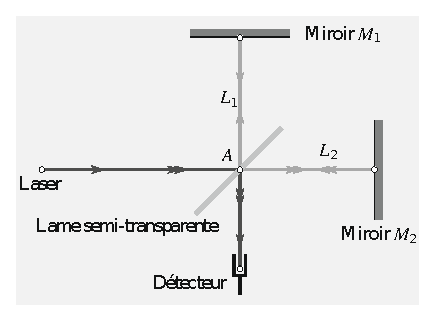
\includegraphics[width=8cm]{Images/interfero.eps}
			\caption{Interféromètre}
		\end{figure}
		En définissant $L_1$ et $L_2$ comme les distances entre le miroir séparateur (lame semi-transparente) et respectivement les miroirs 1 et 2, il est possible de trouver une expression du décalage temporel. Pour ce faire, la formule \eqref{intervalle} doit être réadaptée dans le cas où les distances sont différentes et développée en série de Taylor dans le cas où $\dfrac{v_0}{c} << 1$.
		\begin{equation}
			\Delta t_{BA}^{(i)}
				\quad=\quad
			\dfrac{2}{c}    \cdot    \left(\dfrac{L_2}{1 - \left(\dfrac{v_0}{c}\right)^2} - \dfrac{L_1}{\sqrt{1 - \left(\dfrac{v_0}{c}\right)^2}}\right)
			\label{interf}
		\end{equation}
		En raison de l'imprécision sur $L_1$ et $L_2$ provoquant un déphasage, deux mesures vont être effectuées : une dans un sens ($\Delta t_{BA}^{(i)}$) et l'autre après rotation de $\pi/2$ [radians] par rapport à la première ($\Delta t_{BA}^{(f)}$). Cette rotation permet de permuter les indices $1$ et $2$ dans la formule \eqref{interf} :
		\begin{equation}
			\Delta t_{BA}^{(f)}
				\quad=\quad
			\dfrac{2}{c}    \cdot    \left(   \dfrac{L_1}{1 - \left(\dfrac{v_0}{c}\right)^2} - \dfrac{L_2}{\sqrt{1 - \left(\dfrac{v_0}{c}\right)^2}}   \right)
			\label{interf2}
		\end{equation}
		Ces deux mesures permettent d'effectuer une combinaison linéaire de \eqref{interf} et \eqref{interf2}, éliminant l'imprécision.
		\begin{equation}
			\Delta t_{BA}
				\eq
			\Delta t_{BA}^{(i)} + \Delta t_{BA}^{(f)}
				 \eq
			\dfrac{2}{c} (L_1 + L_2)    \left(   \dfrac{1}{1 - \left(\dfrac{v_0}{c}\right)^2}-\dfrac{1}{\sqrt{1-\left(\dfrac{v_0}{c}\right)^2}} \right)
				\; \approx \;
			\dfrac{L_1 +L_2}{c}\cdot \left(\dfrac{v_0}{c}\right)^2
		\end{equation}
		Il est ainsi possible de calculer le déphasage entre les deux configurations en considérant que $L_1 + L_2 = 2L$ :
		\begin{equation}
			\dfrac{\Delta \phi_{BA}}{2\pi}
				\eq
			\dfrac{\omega}{2\pi}\Delta t_{BA}
				\; \approx \;
			\dfrac{2\pi f}{2 \pi} \cdot \dfrac{2L}{c} \cdot \left(\dfrac{v_0}{c}\right)^2
				\eq
			\dfrac{2L}{\lambda} \cdot \left(\dfrac{v_0}{c}\right)^2
			\label{dephasage}
		\end{equation}
		L'équation \eqref{dephasage} décrit le déphasage entre les signaux à l'arrivée sur l'écran d'observation. Elle dépend de L, supposée égale pour les deux miroirs, de la longueur d'onde émise $\lambda$ et de $v_0$ qui est donc la vitesse du référentiel dans l'éther.

	\subsubsection{Résultats expérimentaux}

		Michelson a utilisé en 1881 des miroirs espacés de 1,2m et une lampe au sodium émettant avec $\lambda = \SI{6000}{\angstrom}$. Il aurait donc dû observer un déphasage de 0.04 radians avec une précision expérimentale de l'odre de 0.01 radians. Or, il n'a jamais rien vu.

		En 1887, une seconde tentative emploie des miroirs éloignés de 11m. Les calculs théoriques prédisaient alors un déphasage de 0,4 radians, soit approximativement: $\Delta \phi^{th} = 2\pi \cdot 0,4 \approx \pi$. On aurait donc dû observer des interférences destructrices entre les deux signaux. Mais ce n'était pas le cas : \textbf{l'hypothèse d'un éther stationnaire est réfutée}.

\subsection{Tentatives pour préserver la théorie de l'éther}

	\subsubsection{L'éther entraîné: Fizeau} \label{Fizeau}

		Faire l'hypothèse de l'éther entraîné consiste à considérer que, dans son mouvement, la Terre emporte avec elle un peu d'éther à la manière dont on emporte de l'eau en passant sa main dans une baignoire. Par conséquent, l'éther se déplace avec la Terre et la vitesse de la Terre par rapport à l'éther n'est plus la même que si elle n'entraînait pas d'éther. Cet entraînement (partiel voir total) provoque un déphasage nul entre les deux faisceaux de l'interféromètre.

		Fizeau a cherché à quantifier cet entraînement par un certain coefficient $k$ à l'aide du dispositif représenté à la figure \eqref{fizeau}. Il s'agit de l'expérience de la double fente de Young à laquelle a été ajouté un lentille optique et un tuyau dans lequel de l'eau (d'indice de réfraction $n=1.33$) s'écoule à une vitesse $v$.
		\begin{figure}[!ht]
			\centering
			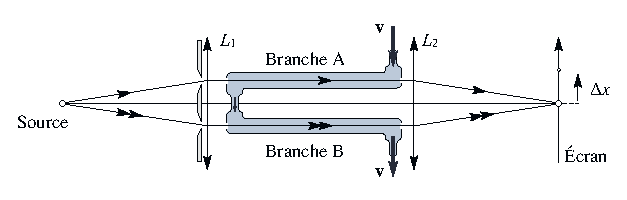
\includegraphics[width=10cm]{Images/fizeau.eps}
			\caption{Expérience de Fizeau}
			\label{fizeau}
		\end{figure}\\
		Les vitesses des faisceaux A et B dans l'eau peuvent ainsi s'écrire comme la vitesse de la lumière dans ce milieu à laquelle il faut ajouter ou retirer l'entraînement de l'éther dû au mouvement de l'eau:
		\begin{equation}
			\left\{
			\begin{array}{ll}
				v_{A} = c/n - k \cdot v
				\\
				v_{B} = c/n + k \cdot v
			\end{array}
			\right.
		\end{equation}
		Le décalage temporel entre les deux faisceau est donc, le terme $k^2v^2$ étant négligeable:
		\begin{equation}
			\Delta t_{AB}
				\eq
			\dfrac{L}{v_A} -\dfrac{L}{v_B}
				\eq
			L \cdot \dfrac{ \left(c/n + k \cdot v \right) \; - \; \left(  c/n - k \cdot v   \right)} { (c/n)^2 \; - \; k^2 \cdot v^2}
				\eq
			k \cdot \dfrac{2Lvn^2 }{c^2}
		\end{equation}
		Le déphasage peut donc se calculer comme suit.
		\begin{equation}
			\left(\dfrac{\Delta \phi}{2\pi}\right)^{\text{Theorique}}
				\eq
			\dfrac{\omega}{2\pi} \cdot \Delta t_{AB}
				\eq
			\nu \cdot \Delta t_{AB}
				\eq
			\dfrac{c}{\lambda} \cdot k \cdot \dfrac{2Lvn^2 }{c^2}
				\eq
			0.23k
		\end{equation}
		Si l'hypothèse de l'éther entraîné est correcte, alors le déphasage théorique doit être égal au déphasage observé expérimentalement qui était de 0.1 avec les valeurs représentées sur le schéma expérimental. Par conséquent, l'éther ne subit qu'un entraînement partiel car $k=0.44 \approx 1- \dfrac{1}{n^2}$ (formule empirique).

		Ce résultat n'est en fait qu'un effet relativiste et il est possible d'obtenir la formule de Fizeau à partir de la théorie de la relativité restreinte.

		Pour résumer brièvement à ce stade:
		\begin{enumerate}
			\item \textbf{$k = 0:$} Éther immobile, réfuté
			\item \textbf{$k = 1 - \dfrac{1}{n^2}$:} Éther partiellement entraîné, investigué par Fizeau (1851)
			\item \textbf{$k = 1$:} Éther totalement entraîné ($v = 0$)
		\end{enumerate}

	\subsubsection{Longueur contractée de Lorentz}

		Une autre tentative pour sauver la théorie de l'éther fut imaginée par Lorentz. En reprenant l'équation \eqref{interf} du décalage temporel entre les deux aller-retours de Gregory, et en considérant ce décalage temporel nul (pour s'accorder avec les faits expérimentaux), Lorentz dériva une expression relativiste:
		\begin{align}
				\Delta t_{BA}
			& =\;
				\dfrac{2}{c}    \cdot    \left(\dfrac{L_B}{1 - (\dfrac{v_0}{c})^2} - \dfrac{L_A}{\sqrt{1 - (\dfrac{v_0}{c})^2}}\right)\\[9pt]
			& =\;
				0
			\quad \textrm{ssi} \quad
			\boxed{
				L_B \eq \dfrac{1}{\sqrt{1 - (\dfrac{v_0}{c})^2}} \cdot L_A
			\eq
				\gamma \cdot L_A
			\; < \;
				L_A
			}
		\end{align}
		Il s'agit bien de la contraction des longueur due à la relativité et ses postulats. Lorentz imagina à tort que cet effet de contraction était dû à une interaction moléculaire et non à un effet de perspective.

\newpage

\section{Maxwell}
\textbf{L'objectif de ce chapitre va être de prouver que les équations de Maxwell ne sont pas en adéquation avec les transformations de Galilée et d'établir les transformations de Lorentz qui résolvent ce problème.}

\subsection{Rappels sur les lois de Maxwell}

Dans le vide (donc pas de charge ni de densité de courant) les équations de Maxwell se présentent sous la forme suivante:
\begin{equation}
\label{maxwell1}
	\Vec{\nabla}\cdot\vec{E} \quad= \quad 0
\end{equation}
\vspace*{-1cm}
\begin{equation}
\label{maxwell2}
	\Vec{\nabla}\cdot\vec{B}\quad =\quad 0
\end{equation}
\vspace*{-1cm}
\begin{equation}
\label{maxwell3}
	\Vec{\nabla}\times\vec{E}    \quad =\quad    - \dfrac{1}{c}\dfrac{\p \vec{B}}{\p t}
\end{equation}
\vspace*{-1cm}
\begin{equation}
\label{maxwell4}
	\Vec{\nabla}\times\vec{B}\quad =\quad \dfrac{1}{c} \cdot \dfrac{\p \vec{E}}{\p t}
\end{equation}

%Équations de propagation de la lumière dans le vide:
%\begin{equation}
%    \label{eqprop1}
%    (\dfrac{1}{c^2}\dfrac{\p ^2}{\p t^2} - \Delta) \vec{E}\quad =\quad 0
%\end{equation}
%\begin{equation}
%    \label{eqprop2}
%    (\dfrac{1}{c^2}\dfrac{\p ^2}{\p t^2} - \Delta) \vec{B}\quad =\quad 0
%\end{equation}
%\paragraph{NB} Les 4 équation de Maxwell peuvent être notées de différentes façons. Plus %précisément les coefficients de $-\dfrac{\p \vec{B}}{\p t}$ et $\dfrac{\p \vec{E}}{\p t}$ peuvent %être différents.

\subsection{Maxwell et Galilée}

Les transformations de Galilée ne permettent pas l'invariance des équations de Maxwell : faire les mêmes expériences dans un référentiel inertiel puis dans un autre en MRU par rapport au premier ne donnerait pas les mêmes résultats selon Galilée. Cela peut s'observer de façon heuristique (sans développement mathématique) et de façon plus formelle (avec développements mathématiques).

\subsubsection{Façon heuristique}

Une onde électromagnétique dans le vide se déplace à la vitesse $c$. Cependant, sous une transformations de Galilée (lors d'un changement de référentiel en MRU par rapport au premier), cette vitesse est modifiée. En effet, la loi d'addition des vitesses autoriserait une onde a se propager plus vite que la lumière. Cela montre bien que les équations de l'électromagnétisme sont elles-mêmes modifiées sous une telle transformation.

\subsubsection{Façon formelle}

De façon plus mathématique que précédemment, il est prouvable que les transformations de Galilées ne permettent pas l'invariance des équations de Maxwell lors d'un changement de référentiel.

Dans la théorie newtonienne, la charge et la force sont deux grandeurs supposées invariantes par changement de référentiel : $F = F'$ et $q = q'$. En reprenant la force de Lorentz, on peut écrire, pour un référentiel $\mathcal{R}$ et un autre référentiel $\mathcal{R'}$ se déplaçant à une vitesse $v_e$ par rapport à $\mathcal{R}$, que la force de Lorentz est invariante:
\[
q \cdot (\vec{E}   + \dfrac{\vec{v_{ch}}}{c}  \times \vec{B} )
	\eqq
q' \cdot (\vec{E'} + \dfrac{\vec{v'_{ch}}}{c} \times \vec{B'})
\]
La quantité de charge ne pouvant varier, on a que $q = q'$. De plus, la vitesse relative des deux référentiels (supposés en MRU) est connue : $v'_{ch} = v_{ch} + v_e$.
\begin{equation}
\vec{E} + \dfrac{\vec{v_{ch}}}{c} \times \vec{B}
\eqq
\vec{E'} + \dfrac{\vec{v_{ch}} + \vec{v_e}}{c} \times \vec{B'}
\label{Lorentz}
\end{equation}
L'équation \eqref{Lorentz} doit être vraie quelle que soit $v_{ch}$ : il est par conséquent possible de dériver l'équation \eqref{E} en posant $v_{ch}=0$. De plus, l'équation \eqref{B} peut être trouvée en remplaçant $B'$ dans l'équation \eqref{Lorentz} grâce à l'équation \eqref{E}.
\begin{equation}
\vec{E'} \eqq \vec{E} -\dfrac{\vec{v_e}}{c} \times \vec{B}
\label{E}
\end{equation}
\begin{equation}
\vec{B'} \eqq \vec{B}
\label{B}
\end{equation}
Ce résultat ne pose à priori pas de problème : observer un champ électrique différent parce qu'on se déplace n'a rien de problématique. Le problème vient du fait que les équations de Maxwell ne sont plus invariantes. En reprenant l'équation \eqref{maxwell1}, on peut écrire que :
\[
\nabla' \cdot \vec{E'} \eqq \nabla' \cdot (\vec{E} + \dfrac{\vec{v_e}}{c} \times \vec{B})
\]
Pour pouvoir transformer ce $\nabla'$, il faut voir ce que vaut la dérivée $\dfrac{\p}{\p x'}$ en fonction de $x$ et $ct$:
\[
\label{transfogalilee}
\left\{
\begin{array}{ll}
	t = t' \\
	\vec{x'} = \vec{x} + \vec{v_e} \cdot t
\end{array}
\right.
\quad \Rightarrow \quad
\dfrac{\p}{\p x'}  \eq
\dfrac{\p}{\p x} \dfrac{\p x}{\p x'}
+
\dfrac{\p}{\p ct} \dfrac{\p ct}{\p x'}
\eq
\dfrac{\p}{\p x}
\]
Par conséquent,
\[
\nabla' \cdot \vec{E'}
	\eq
\nabla \cdot \vec{E} -  \nabla \cdot \dfrac{\vec{v_e}}{c} \times \vec{B}
	\eq
-  \nabla \cdot \dfrac{\vec{v_e}}{c} \times \vec{B}
	\eq
\vec{v_e} \cdot (\nabla \times \vec{B})
	\; \neq \;
0
\]
Cette équation de Maxwell n'est donc pas covariante (on ne la retrouve pas sous la même forme) sous transformation de Galilée (lorsqu'on passe d'un référentiel à l'autre de la façon décrite par Galilée). D'autres transformations doivent être utilisées et c'est en Lorentz que Maxwell trouve son bonheur.

\subsection{Maxwell et Lorentz}

Commençons par énoncer les transformations de Lorentz classiques appliquées au temps et à l'espace selon l'axe x\footnote{L'extension aux autres dimensions n'est qu'une affaire de projection de la vitesse selon les différents axes, voir TPs}, avec $\gamma = (1-(v/c)^2)^{-1/2}$:
\begin{equation}
\label{lorentz1D}
\left\{
	\begin{array}{ll}
		ct' \eqq  \gamma \cdot (ct \;+\; \dfrac{v_0}{c} x)\\[7pt]
		x'  \eqq  \gamma \cdot (x  \;+\; \dfrac{v_0}{c} t)
	\end{array}
\right.
\end{equation}
Il est possible de montrer\footnote{Démonstration triviale laissée à la sagacité de l'infortuné lecteur.} que les équations de Maxwell sont invariantes sous les transformations de Lorentz appliquées comme suit:
\begin{equation}
\left\{
	\begin{array}{ll}
		\vec{E'}
			\eqq
		\gamma \cdot  (\vec{E} -\dfrac{\vec{v_0}}{c} \times \vec{B})
			\; + \;
		\dfrac{(1-\gamma)}{v_{0}^2} \cdot (\vec{v_0}\vec{E}) \cdot \vec{v_0}
		\\[7pt]
		\vec{B'}
			\eqq
		\gamma \cdot (\vec{B} +\dfrac{\vec{v_0}}{c} \times \vec{E})
			\; + \;
		\dfrac{(1-\gamma)}{v_{0}^2} \cdot (\vec{v_0}\vec{B}) \cdot \vec{v_0}
	\end{array}
\right.
\label{champs}
\end{equation}
\paragraph{Remarques: }
\begin{enumerate}
\item Le lecteur sagace\footnote{Quand il aura dûment fini sa démonstration.} aura déjà remarqué l'antisymétrie de l'expression \eqref{champs} entre $\vec{E}$ et $\vec{B}$: effectuer le changement de variables $(\vec{E},\vec{B}) \rightarrow (\vec{B},-\vec{E})$ ne modifie pas l'expression. Cette antisymétrie est une des raisons qui nous confortent dans l'utilisation des transformations de Lorentz car la nature aime les symétries.

\item Les équations du système \eqref{champs} peuvent être séparées selon leurs composantes parallèles et perpendiculaires à la vitesse de propagation $\vec{v_0}$.
\begin{equation}
\left\{
	\begin{array}{llll}
		E'_\parallel  \eqq  E_\parallel
	\\[7pt]
		B'_\parallel  \eqq  B_\parallel
	\\[7pt]
		E'_\perp   \eqq   \gamma \left( E_\perp -\dfrac{\vec{v_0}}{c} \times \vec{B} \right) + \dfrac{(1-\gamma)}{v_{0}^2}(\vec{v_0}\vec{E})\vec{v_0}
	\\[7pt]
		B'_\perp   \eqq   \gamma \left( B_\perp +\dfrac{\vec{v_0}}{c} \times \vec{E} \right) + \dfrac{(1-\gamma)}{v_{0}^2}(\vec{v_0}\vec{B})\vec{v_0}
	\end{array}
\right.
\end{equation}
Il devient alors évident que seules les composantes perpendiculaire au mouvement sont affectées par la correction relativiste.
\end{enumerate}
\subsection{Les deux principes de la relativité d'Einstein (1905)}
\[
	\boxed{
		\begin{array}{ll}
			1. \textrm{\textbf{ Tous les référentiels inertiels sont équivalents. }} \\
			2. \textrm{\textbf{ La vitesse de la lumière est universelle. }}
		\end{array}
	}
\]
Le résultat nul de Michelson devient donc évident à la lumière de ces deux principes. Il est très important de noter que ces deux principes reposent sur l'hypothèse d'un espace-temps homogène. Ces principes ne peuvent donc pas expliquer des phénomènes dans un champ de gravitation car celui-ci exprime la courbure de l'espace-temps, il n'est donc plus homogène.\footnote{A explorer dans la suite du cours...à moins que vous soyez vraiment sagaces} Nous avons désormais abordé trois visions de l'espace temps:
\begin{enumerate}
	\item Selon \textbf{Newton:} L'espace est différent du temps, le temps est absolu et l'espace définit un référentiel absolu.
	\item Selon \textbf{Galilée:} Le temps est absolu mais il existe de multiples référentiels équivalents. On peut passer de l'un à l'autre via les transformations de Galilée.
	\item Selon \textbf{Einstein:} L'espace et le temps sont placés sur un pied d'égalité, à condition de multiplier $t$ par $c$. Il en découle les deux postulats énoncés ci-dessus.
\end{enumerate}

\subsection{Les transformations de Lorentz}

Il est possible d'aboutir aux transformations de Lorentz \eqref{lorentz1D} à partir des deux seuls postulats d'Einstein. Tout d'abord l'homogénéité de l'espace nous informe sur le caractère linéaire\footnote{Contre-exemple: la relation entre position et temps est quadratique lorsqu'on étudie la gravité sur Terre: $y = g\dfrac{t^2}{2}$. La gravité déformant l'espace-temps le prive de son caractère homogène.} des expressions à développer. Sachant qu'espace et temps seront désormais deux dimensions tout à fait comparable, posons deux expressions générales de $x'$ et $t'$:
\[
	\left\{
		\begin{array}{ll}
			t' \eqq   at  \quad +\quad bx  \\
			x' \eqq   a't \quad+\quad  b'x
		\end{array}
	\right.
\]
Comme dit précédemment, pour comparer temps et espace il est nécessaire de multiplier $t$ par $c$.
\[
	\left\{
		\begin{array}{ll}
			ct' \eqq   act  \quad +\quad bx \\
			x'  \eqq   a'ct \quad +\quad b'x
		\end{array}
	\right.
\]
Regardons maintenant la propagation de la lumière selon l'axe $x$ de deux référentiels $\mathcal{R}$ et $\mathcal{R'}$. Il est correct d'écrire
\begin{equation}
	\left\{
		\begin{array}{ll}
		x' = ct'
		\\
		x = ct
		\end{array}
		\Rightarrow \quad act \; + \; bx   \eq   a'ct \; + \; b'x
		\quad \Rightarrow \quad act \; + \; bct   \eq   a'ct \; + \; b'ct
	\right.
	\label{max1}
\end{equation}
En reprenant l'équation \eqref{max1} et en tenant le même raisonnement pour de la lumière se propageant dans la direction $-x$, le système suivant est obtenu:
\[
	\left\{
		\begin{array}{ll}
			a'+ b'\quad =\quad a + b\\
			a'- b' \eqq  -a + b
		\end{array}
	\right.
\]
Dès lors $a = b'$ et $a' = b$ : le temps n'est plus absolu et dépend bel et bien de l'espace de l'espace. En résumé :
	\[
		\left\{
			\begin{array}{ll}
				ct' \eqq  act+bx\\
				x'  \eqq  bct + ax
			\end{array}
		\right.
	\]
En considérant un observateur au repos dans $\mathcal{R}$ en $x = 0$ la relation $x' = v_0 t'$ est obtenue. Par conséquent, $bct = v_0 at$ et:
	\begin{equation}
		\left\{
			\begin{array}{ll}
				ct' \eqq  a \cdot (ct+\dfrac{v_0}{c}x)\\
				x'  \eqq  a \cdot (v_0 t + x)
			\end{array}
		\right.
		\label{rels}
	\end{equation}
Il faut maintenant supposer que c'est $\mathcal{R}$ et non plus $\mathcal{R'}$ qui se meut (cette fois à une vitesse $-v_0$ : postulat d'équivalence des référentiels inertiels). Les relations \eqref{rels} doivent rester équivalentes si $v_0 \rightarrow -v_0$ et si $t'$ et $t$ ainsi que $x'$ et $x$ sont inversés:
	\begin{align}
		x \;
		&= \; a \cdot \left(-v_0 t' + x'\right)\\[7pt]
		&= \; a \cdot \Big[-v_0 \cdot \left(    at + a \dfrac{v_0}{c^2} x\right) \; + \;  \left(a v_0 t + a x\right)\Big]\\[7pt]
		&= \; a^2 \cdot  \left(1 - \dfrac{v_0^2}{c^2}\right) \cdot x
	\end{align}
L'expression de $\gamma$ est donc retrouvée :
	\begin{equation}
		a \eq \gamma \eq \dfrac{1}{\sqrt{1-\dfrac{v_{0}^2}{c^2}}}
	\end{equation}
On note finalement les transformations de Lorentz comme suivant :
	\begin{equation}
		\boxed{
		\left\{
			\begin{array}{ll}
				ct' \eqq  \gamma \cdot (ct+\dfrac{v_0}{c}x)\\
				x'  \eqq  \gamma \cdot (v_0 t + x)
			\end{array}
		\right.
		}
			\quad \Leftrightarrow \quad
		\boxed{
		\begin{pmatrix}
			cdt'\\
			dx'
		\end{pmatrix}
			\eq \gamma \cdot
		\begin{pmatrix}
			1 & \beta \\
			\beta & 1
		\end{pmatrix}
		\begin{pmatrix}
			c dt\\
			x
		\end{pmatrix}
		}
		\label{relations}
	\end{equation}

\subsection{Vérification de postulats d'Einstein} \label{verif}

Les transformations de Lorentz garantissent-elles les deux principes de relativité d'Einstein? Il est possible de vérifier cela :
\begin{enumerate}
	\item \textbf{Principe d'équivalence des référentiels inertiels} : \\
	Les transformations de Lorentz doivent rester les mêmes si, à la place de considérer $\mathcal{R'}$ fixe et $\mathcal{R}$ en mouvement, on considère $\mathcal{R}$ fixe et $\mathcal{R'}$ en mouvement. Pour illustrer cela sous forme d'équation, il faut effectuer des changements de variables dans les transformations de Lorentz: $x \leftrightarrow x'$, $t \leftrightarrow t'$ et $v_0 \rightarrow -v_0$ en se rappelant que $\xi = v_0 / c$.
	\[
		\begin{pmatrix}
			cdt'\\
			dx'
		\end{pmatrix}
			\eq
		\begin{pmatrix}
			\ch(\xi) & \sh(\xi) \\
			\sh(\xi) & \ch(\xi)
		\end{pmatrix}
		\begin{pmatrix}
			c dt\\
			x
		\end{pmatrix}
	\quad \longrightarrow \quad
		\begin{pmatrix}
			c dt\\
			x
		\end{pmatrix}
	\eq
		\begin{pmatrix}
			\ch(-\xi) & \sh(-\xi) \\
			\sh(-\xi) & \ch(-\xi)
		\end{pmatrix}
		\begin{pmatrix}
			cdt'\\
			dx'
		\end{pmatrix}
	\]
	L'expression obtenue peut être encore modifiée. En effet, on peut se souvenir (ou redémontrer) la propriété de la matrice $L(\xi)$ : $L(-\xi) = L^{-1}(\xi)$. La même expression des équations de Lorentz est alors ré-obtenue, prouvant que le postulat d'équivalence des référentiels inertiels est vérifié par les transformations de Lorentz.

	\item \textbf{Universalité de la vitesse de la lumière} : \\
	Les transformations de Lorentz doivent interdire de dépasser la vitesse de la lumière. Pour prouver cela, il faut considérer deux transformations de Lorentz successives définies par les matrices $L(\xi_1)$ et $L(\xi_2)$: un référentiel $\mathcal{R}$ est fixe, le référentiel $\mathcal{R'}$ se déplace à une vitesse $v_1$ par rapport à $\mathcal{R}$ et le référentiel $R''$ se déplace à une vitesse $v_2$ par rapport à $\mathcal{R'}$.\footnote{Tout selon le même axe} Le changement de coordonnées entre $\mathcal{R}$ et $R''$ est:
	\[
		\begin{pmatrix}
			cdt'\\
			dx'
		\end{pmatrix}
			\eq
		L(\xi_2) \cdot L(\xi_1) \cdot
		\begin{pmatrix}
			c dt\\
			x
		\end{pmatrix}
			\eq
		L(\xi_2 + \xi_1) \cdot
		\begin{pmatrix}
			c dt\\
			x
		\end{pmatrix}
	\]
	La dernière égalité peut être vérifiée en effectuant le produit matriciel et en utilisant quelques formules de trigonométrie hyperbolique. La question est maintenant de connaître la vitesse du référentiel $R''$ par rapport au référentiel $\mathcal{R}$.\footnote{Galilée affirmerait que $v_{12} = v_{1} + v_{2}$} Avant d'entamer la suite, il est bon de rappeler les égalités \eqref{ega} et \eqref{trigoTan}:
	\begin{equation}
		\tanh(\xi_i) \eq \beta_i \eq v_i/c
		\label{ega}
	\end{equation}
	\begin{equation}
		\tanh(\xi_1 + \xi_2) \eq
		\dfrac{\tanh(\xi_1) \;+\; \tanh(\xi_2)}{1 \;+\; \tanh(\xi_1) \cdot \tanh(\xi_2)}
		\label{trigoTan}
	\end{equation}
	Connaissant ces égalités, il est alors possible de trouver la formule \textbf{d'addition relativiste des vitesses} en exprimant la vitesse $v_{12}$ ($R''$ par rapport à $\mathcal{R}$) en fonction des vitesses $v_{1}$ ($\mathcal{R'}$ par rapport à $\mathcal{R}$) et $v_{2}$ ($R''$ par rapport à $\mathcal{R'}$) :
	\begin{equation}
		\dfrac{v_{12}}{c}
	\eq
		\tanh(\xi_1 + \xi_2)
	\eq
		\dfrac{v_{1}/c \;+\; v_{2}/c}{1 \;+\; \dfrac{v_1}{c} \cdot \dfrac{v_2}{c}}
	\quad \Leftrightarrow \quad
		\boxed{
			v_{12}
		\eq
			\dfrac{v_{1} \;+\; v_{2}}{1 \;+\; v_1v_2 / c^2}
		}
	\label{addVit}
	\end{equation}
	On peut ainsi prouver qu'il est impossible de dépasser la vitesse de la lumière : si une des des deux vitesses vaut $c$, alors $v_{12}$ vaut également $c$ :
	\[
		v_{12}
	\eq
		\lim_{v_2\to c} \dfrac{v_{1} \;+\; v_{2}}{1 \;+\; v_1v_2 / c^2}
	\eq
		\dfrac{v_{1} \;+\; c}{1 \;+\; v_1 / c}
	\eq
		c
	\]
	Dans le cas où $v_{1}$ et $v_{2}$ sont faibles comparé à $c$, le dénominateur de l'expression dérivée en \eqref{addVit} tend vers 1 et on retombe bien sur l'addition classique des vitesses.
\end{enumerate}

\subsection{Application de l'addition relativiste des vitesses à Fizeau}

En reprenant l'expérience de Fizeau (cfr. \eqref{Fizeau}), il est possible d'exprimer la vitesse $v_A$, c'est-à-dire la vitesse de la lumière dans un tube dont l'eau s'écoule à une vitesse $v_0$ dans le sens inverse au sens de la propagation de la lumière:
\[
	v_A
		\eq
	\dfrac{c/n \;-\; v_0}{1 \;-\; \dfrac{v_0}{cn}}
		\quad \overset{Taylor}{\approx} \quad
	(c/n \;-\; v_0) \cdot (1 \;+\; \dfrac{v_0}{cn})
		\eq
	\dfrac{c}{n} - v_0 + \dfrac{v_0}{n^2} - \dfrac{v_0^2}{cn}
		\quad \overset{v_0<<c}{\approx} \quad
	\dfrac{c}{n} - v_0 + \dfrac{v_0}{n^2}
		\eq
	\dfrac{c}{n} - k \cdot v_0
\]
On voit ainsi que le coefficient d'entraînement $k$ de l'éther par une substance d'indice de réfraction $n$ est équivalent au facteur trouvé par la relativité : $k = 1-\dfrac{1}{n^2}$

\newpage

\section{Effet d'aberration}
\subsection{Description du phénomène}

	Cette section décrit en détail l'effet d'aberration qui concerne les téléscopes. Plus précisément, l'objet d'étude sera ici l'observation d'une étoile se trouvant à la verticale d'un télescope sur Terre. Dans le cas d'une vitesse relative de l'étoile par rapport à la Terre nulle, le télescope doit être disposé à la verticale pour observer l'étoile.

	Cependant, dans le cas d'une vitesse relative non-nulle, le télescope doit être incliné selon un certain angle $\alpha$ par rapport à la verticale afin d'observer l'étoile. La figure \ref{aber} illustre ce phénomène.

	\begin{figure}[!ht]
		\centering
		
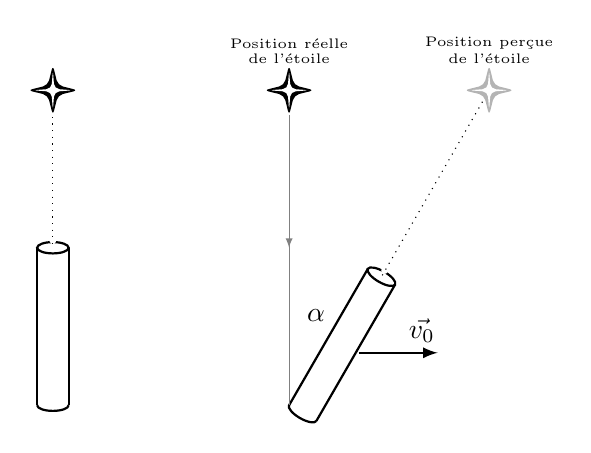
\begin{tikzpicture}[scale=0.4]
  \draw [thick] (0,5) -- (0,0)  (1,0) -- (1,5);
  \draw [thick] (.5,5) ellipse (0.5 and 0.18);
  \draw [thick] (0,0) arc (180:360:0.5 and 0.18);
  \draw [white] node at (0.5,5.2) {\tiny{$\bullet$}};
  \draw [dotted] (.5,10)--(.5,5);
  \polstar[rounded corners=0.64mm]{0.8}{(.5,10)}


  \begin{scope}[shift={(8,0)}]
    \begin{scope}[rotate=-30]
      \draw [thick] (0,5) -- (0,0)  (1,0) -- (1,5);
      \draw [thick] (.5,5) ellipse (0.5 and 0.18);
      \draw [thick] (0,0) arc (180:360:0.5 and 0.18);
      \draw [white] node at (0.5,5.2) {\tiny{$\bullet$}};
      \draw [dotted] (.5,11.835680518387326)--(.5,5);
      %\polstar[rounded corners=0.64mm]{0.8}{(.5,10.823762841892224)}
    \end{scope}
    \draw [help lines, -latex] (0,9.2) -- (0,5);
    \draw [help lines] (0,5.1) -- (0,0);
    \polstar[rounded corners=0.64mm]{0.8}{(0,10)}
    \polstar[rounded corners=0.64mm, fill=\rgb{180}{180}{180}]{0.8}{(6.35085296,10)}
    \centerarc[help lines] (0,0) (2.5,60,90)
    \node [above] at (70:2.5) {$\alpha$};
    \draw [thick, -latex](0,0)++(-30:1)++(60:2.5)++(0.1,0)--++(2,0) node [above] {$\vec{v_0}$} --++(0.5,0);

    \node [above] at (0,11) {\tiny{Position réelle}};
    \node at (0,11) {\tiny{de l'étoile}};

    \node [above] at (6.35085296,11) {\tiny{Position perçue}};
    \node at (6.35085296,11) {\tiny{de l'étoile}};
  \end{scope}
\end{tikzpicture}

		\caption{Schéma de l'effet d'aberration}
		\label{aber}
	\end{figure}

\subsection{Explication newtonienne}

	En supposant un éther stationnaire, Bradley estime que la Terre (télescope) reçoit un <<vent d'éther>> en raison de son déplacement dans un éther stationnaire. Il calcule donc l'angle d'inclinaison du télescope en utilisant la loi d'addition des vitesses dans le cadre d'un temps absolu.
	\begin{figure}[!ht]
		\centering
		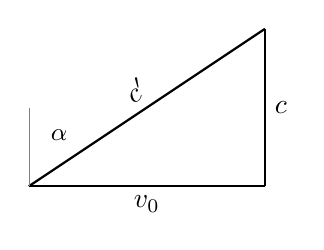
\begin{tikzpicture}
  \draw [thick] (3,0) -- (0,0);
  \node [below] at (1.5,0) {$v_0$};

  \draw [thick] (3,2) -- (0,0);
  \node [anchor=south,rotate=atan(2/3)] at (1.5,1) {$c'$};

  \draw [thick] (3,2) -- (3,0);
  \node [right] at (3,1) {$c$};

  \draw [help lines] (0,0) -- (0,1);
  \centerarc[help lines] (0,0) (0.6,atan(2/3),90)
  \node [above] at (50:0.6) {\small{$\alpha$}};
\end{tikzpicture}

		\caption{Effet d'aberration selon Bradley}
		\label{aber2}
	\end{figure}
	\[\tan(\alpha) \eq \dfrac{v_0}{c} \; \approx \; 10^{-4} \]

\subsection{Explication relativiste}

	Le résultat obtenu par Bradley ne coïncide pas avec le second principe relativiste: la vitesse de la lumière n'est pas universelle dans son explication. Einstein refait l'exercice en incorporant son postulat : il inclut le temps dans le schéma et obtient un tout autre résultat:
	\begin{figure}[!ht]
		\centering
		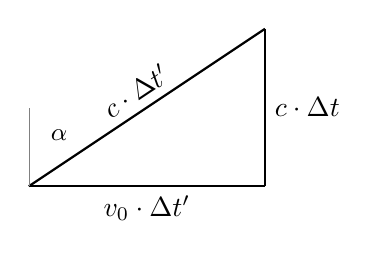
\begin{tikzpicture}
  \draw [thick] (3,0) -- (0,0);
  \node [below] at (1.5,0) {$v_0 \cdot \Delta t'$};

  \draw [thick] (3,2) -- (0,0);
  \node [anchor=south,rotate=atan(2/3)] at (1.5,1) {$c \cdot \Delta t'$};

  \draw [thick] (3,2) -- (3,0);
  \node [right] at (3,1) {$c \cdot \Delta t$};

  \draw [help lines] (0,0) -- (0,1);
  \centerarc[help lines] (0,0) (0.6,atan(2/3),90)
  \node [above] at (50:0.6) {\small{$\alpha$}};
\end{tikzpicture}

		\caption{Effet d'aberration selon Einstein}
		\label{aber3}
	\end{figure}
	\[ \sin(\alpha)  \eq  \dfrac{v_0}{c}\]
	\[ \tan(\alpha)
		\eq
	\dfrac{\sin(\alpha)}{\cos(\alpha)}
		\eq
	\dfrac{\sin(\alpha)}{\sqrt{1-\sin^2(\alpha)}}
		\eq
	\dfrac{v_0 / c}{\sqrt{1-(v_0/c)^2}}
		\eq
	\gamma \cdot \dfrac{v_0}{c}\]
	Or, $\tan(\alpha) = \dfrac{v_0\cdot \Delta t'}{c \cdot \Delta t}$. Par conséquent, en reprenant l'expression du dessus de $\tan (\alpha)$, on obtient la dilatation du temps: $\Delta t' = \gamma \Delta t$
\newpage

\section{Conséquences des transformations de Lorentz}

\subsection{Transformation selon un seul axe}

	Reprenons la transformation de Lorentz en une dimension selon l'axe x sous forme matricielle:
	\begin{equation}
		\begin{pmatrix}
			c \cdot \Delta t\\
			\Delta x
		\end{pmatrix}
		\eq
		\gamma \cdot
		\begin{pmatrix}
			1 & \beta \\
			\beta & 1
		\end{pmatrix}
		\begin{pmatrix}
			c \cdot \Delta t'\\
			\Delta x'
		\end{pmatrix}
		\quad \textrm{avec} \quad \beta = \dfrac{v_0}{c} \quad \textrm{et} \quad \gamma = \dfrac{1}{\sqrt{1-(v_0/c)^2}}
		\label{trans1D}
	\end{equation}
	Plusieurs conséquences sont directement observables dans les référentiels $\mathcal{R}$ (considéré fixe) et $\mathcal{R'}$ (considéré en mouvement selon l'axe x à une vitesse $v_0$) reliés par les équations \eqref{trans1D}:
	\begin{enumerate}
		\item \textbf{La simultanéité est relative}\\
			En supposant deux évènements simultanés dans un des deux référentiels (i.e. $\Delta t' = 0$), il est possible de déterminer l'intervalle de temps entre les deux même évènements dans l'autre référentiel grâce à la relation \eqref{trans1D}:
			\begin{equation}
				c \cdot \Delta t \eq \gamma \cdot \beta \cdot \Delta x'
			\end{equation}
			Cet intervalle de temps étant non-nul (à moins de considérer deux évènements les mêmes: même endroit, même temps), on en déduit que deux évènements ayant lieu au même instant en deux endroits distincts de l'espace dans un certain référentiel ne se produisent pas en même temps dans un référentiel en mouvement par rapport au premier. Le simultanéité de deux évènement n'est donc pas absolue ; elle est relative.

		\item \textbf{Contraction des longueurs}\\
			Soit une barre immobile dans le référentiel $\mathcal{R}$. Pour mesurer sa longueur dans le référentiel $\mathcal{R'}$, il faut mesurer deux évènements simultanés dans ce référentiel (i.e. $\Delta t' = 0$).
			En reprenant l'équation \eqref{trans1D}, on en déduit que:
			\begin{equation}
				\begin{pmatrix}
					c \cdot \Delta t\\
					\Delta x
				\end{pmatrix}
			\eq
				\gamma \cdot
				\begin{pmatrix}
					1 & \beta \\
					\beta & 1
				\end{pmatrix}
				\begin{pmatrix}
					0\\
					\Delta x'
				\end{pmatrix}
			\quad \Rightarrow \quad
					\Delta x \eq \gamma \cdot \Delta x'
			\quad \Leftrightarrow \quad
					\Delta x' \eq \gamma^{-1} \cdot \Delta x
			\; < \; \Delta x
			\end{equation}
			Par conséquent, si la longueur d'une barre dans son \textbf{référentiel propre}\footnote{çàd le référentiel où la barre est au repos ($\mathcal{R}$ dans notre cas)} est connue, la longueur de cette barre dans un référentiel en mouvement sera toujours plus petite que celle dans le référentiel propre:
			\begin{itemize}
				\item $L(\tilde{\mathcal{R}}) < L(\mathcal{R})$: la longueur de la barre est ici fixée dans le référentiel $\mathcal{R}$: la longueur sera donc plus petite dans le référentiel $\tilde{\mathcal{R}}$
				\item $\tilde{L}(\mathcal{R}) < \tilde{L}(\tilde{\mathcal{R}})$: la longueur de la barre est ici fixée dans le référentiel $\tilde{\mathcal{R}}$: la longueur sera donc plus petite dans le référentiel $\mathcal{R}$
			\end{itemize}
			\textbf{Il est à noter que la barre n'est pas mécaniquement déformée: la contraction de longueur n'est qu'une question de perspectives.}

		\item \textbf{Dilatation du temps}
			Il y a deux façons de prouver la dilatation du temps:

				\textbf{Aberration}:\\ En appliquant le théorème de Pythagore au triangle se trouvant à la figure \eqref{aber3}.
				\[
					c \cdot \Delta t
						\eq
					\left( c^2 \cdot (\Delta t')^2 \; - \; v_0^2 \cdot (\Delta t')^2\right) ^{1/2}
						\eq
					c \cdot \Delta t' \cdot \left( 1 \; - \; v_0^2 / c^2\right) ^{1/2}
						\eq
					c \cdot \Delta t' \cdot \gamma^{-1}
				\]
				Par conséquent:
				\begin{equation}
					\Delta t' \eq \gamma \cdot \Delta t \; > \; \Delta t
					\label{DilTemps}
				\end{equation}

				\textbf{Transformation de Lorentz}:\\ En posant $\Delta x = 0$ dans l'équation \eqref{trans1D} \footnote{Ce qui peut être physiquement représenté par une horloge posée sur une table}, l'équation \eqref{DilTemps} peut être retrouvée :
				\[
				\left\{
					\begin{array}{ll}
						c \Delta t \eq \gamma \cdot
						\big[
							c \Delta t' + \beta \Delta x'
						\big]
						\\[7pt]
						0 \eq \gamma \cdot
						\big[
							\beta c \Delta t' + \Delta x'
						\big]
					\end{array}
				\right.
				\; \Leftrightarrow \;
					c \Delta t \eq \gamma \cdot
					\big[
						c \Delta t' - \beta^2 c \Delta t'
					\big]
					\eq \gamma \cdot
					(1 - \beta^2) \cdot c \Delta t'
				\; \Leftrightarrow \;
					\Delta t' \eq \gamma \Delta t
				\]
				De façon similaire à la contraction des longueurs, si l'intervalle de temps entre deux évènements dans le référentiel propre aux évènements \footnote{la vitesse relative des deux évènements et leur vitesse par rapport au référentiel est nulle} est connu, l'intervalle de temps dans tout autre référentiel sera toujours plus grand que que celui dans le référentiel propre:
				\begin{itemize}
					\item $T(\tilde{\mathcal{R}}) > T(\mathcal{R})$: l'intervalle entre les deux évènements est ici fixé dans le référentiel $\mathcal{R}$: l'intervalle sera donc plus grand dans le référentiel $\tilde{\mathcal{R}}$
					\item $\tilde{T}(\mathcal{R}) > \tilde{T}(\tilde{\mathcal{R}})$: l'intervalle entre les deux évènements est ici fixé dans le référentiel $\tilde{\mathcal{R}}$: l'intervalle sera donc plus grand dans le référentiel $\mathcal{R}$
				\end{itemize}
	\end{enumerate}

\subsection{Application: observation des muons cosmiques} \label{Muons}
	\subsubsection{Mais les muons, c'est quoi Jamie?}

		Eh bien Fred, c'est très simple. En fin de vie, une étoile peut devenir une supernova: une immense explosion libérant de la matière dont des protons. Ces protons, hautement énergétiques, rencontrent parfois les protons de l'atmosphère terrestre. Surviennent alors une série de transformations des deux protons qui donnent finalement naissance à un muon: une particule de temps de vie propre\footnote{temps de vie dans son propre référentiel} $\tau \eq 2 \cdot 10^{-6}$ secondes.

	\subsubsection{Observation des muons}

		Une fois créés à une dizaine de kilomètres de la surface terrestre, les muons parcourent une certaine distance à une vitesse proche de celle de la lumière ($V_{moy,\mu} = 0.9999 \cdot c$) avant de se désintégrer:
		\begin{equation}
			\textrm{dist} \eq V_{moy,\mu} \; \cdot \; \tau_\mu \; \approx \; c \cdot 2 \cdot 10^{-6} \eq 600 \; m
			\label{distMu}
		\end{equation}
		Il serait donc impossible d'observer un muon sur Terre ailleurs que dans la haute atmosphère. Cependant, ces muons sont facilement observables dans un laboratoire sur la surface terrestre: le calcul \eqref{distMu} est erroné. En effet, le temps de vie utilisé (celui du muon dans son propre référentiel) doit être modifié: on n'observe pas le muon dans son propre référentiel:
		\begin{equation}
			\tau' = \gamma^{-1} \cdot \tau
				\quad \Leftrightarrow \quad
			\textrm{dist}
				\eq
			V_{moy,\mu}  \cdot \gamma \cdot \tau
				\eq
			600 \cdot 70 \textrm{ [m]} \; > \; \textrm{dist(atmo,labo)}
				\eq
			10 \textrm{ [km]}
		\end{equation}
		Une autre façon de voir cela est d'utiliser la contraction des longueurs: dans son propre référentiel, le muon existe pendant $10^{-6}$ secondes et la distance atmosphère-laboratoire est contractée:
		\begin{equation}
			d_{\mu} \eq \gamma^{-1} \cdot 10 \textrm{ [km]} \; \approx \; 140 \textrm{ [m]}
		\end{equation}
		Dans son propre référentiel, le muon peut parcourir 600 mètres. Il n'a donc aucune difficulté à être détecté dans un laboratoire se trouvant, pour lui, à 140 mètres de l'endroit où il est créé.

\subsection{Application: le paradoxe des jumeaux}

	Soit un observateur A sur Terre et son jumeau B qui part en voyage dans l'espace. La vitesse de B étant supérieure à celle de A, B devrait être plus jeune à son retour sur Terre. Cependant, le principe de relativité autorise de considérer B au repos et A en mouvement...par conséquent ce devrait être A qui devrait être plus jeune au retour de B.

	La paradoxe n'en est en fait pas un: l'accélération que subit B est relativiste (ceci sera traité plus en détail dans le cours de relativité générale et dans le chapitre sur la dynamique relativiste). Par conséquent, en effectuant une accélération, B revient effectivement plus jeune que A sur Terre.

\subsection{Transformation selon deux axes}

	\subsubsection{Rotations consécutives}

		Supposons un point sur lequel deux pseudo-rotations sont effectuées (une selon l'axe z et l'autre selon l'axe y). La matrice de rotation totale s'écrit comme le produit des deux rotations:
		\begin{equation}
			R_{tot} =
			\begin{pmatrix}
			\ch(\xi_2) & \sh(\xi_2) & 0\\
			\sh(\xi_2) & \ch(\xi_2) & 0\\
			0 & 0 & 1
			\end{pmatrix}
			\cdot
			\begin{pmatrix}
			\ch(\xi_1) & 0 & \sh(\xi_1)\\
			0 & 1 & 0\\
			\sh(\xi_1) & 0 & \ch(\xi_1)
			\end{pmatrix}
		\end{equation}
		Comme $\xi_1 , \xi_2$ sont proches de zéro, le cosinus hyperbolique peut être approximé par 1 ($\ch(\xi_{1,2}) \approx 1$)et le sinus hyperbolique par son angle ($\sh(\xi_{1,2}) \approx \xi_{1,2}$). Ces deux approximations donnent la matrice de pseudo-rotation suivante:
		\begin{equation}
			R_{tot} \approx
			\begin{pmatrix}
			0     & \xi_2 & \xi_1\\
			\xi_2 &  0    & \xi_1 \cdot \xi_2\\
			\xi_1 &  0    & 0
			\end{pmatrix}
			\eq
			\underbrace{
				\begin{pmatrix}
				0     & \xi_2 & \xi_1\\
				\xi_2 &  0    & \dfrac{\xi_1 \cdot \xi_2}{2}\\
				\xi_1 &  \dfrac{\xi_1 \cdot \xi_2}{2}    & 0
				\end{pmatrix}
			}_{\textrm{matrice symétrique}}
			+
			\underbrace{
				\begin{pmatrix}
				0 & 0 & 0\\
				0 & 0    & \dfrac{\xi_1 \cdot \xi_2}{2}\\
				0 & -\dfrac{\xi_1 \cdot \xi_2}{2}   & 0
				\end{pmatrix}
			}_{\textrm{matrice antisymétrique}}
		\end{equation}

	\subsubsection{Conséquences de la matrice de rotation totale}
		En effectuant deux pseudo-rotations puis leurs inverses, comme représenté à la figure\eqref{rotationXi}, on ne revient pas au même point de départ: on a effectué une rotation, ce qui est contre-intuitif.
		\begin{figure}[!ht]
			\centering
			\begin{tikzpicture}
  \draw[latex-latex] (0,4) node[left] {$\vec{y}$} -- (0,0) -- (4,0) node[below] {$\vec{x}$};
  \begin{scope}[shift={(7,0)}, scale=3]
    \draw [thick,latex-](0,0) -- (1,0);
    \draw [thick,latex-](1,0) -- (1,1);
    \draw [thick,latex-](1,1) -- (0,1);
    \draw [thick,latex-](0,1) -- (0,0);
    \node [below] at (0.5,0) {$L_x(-\xi_2)$};
    \node [above] at (0.5,1) {$L_x(\xi_2)$};
    \node [left]  at (0,0.5) {$L_y(\xi_1)$};
    \node [right] at (1,0.5) {$L_y(-\xi_1)$};
  \end{scope}
\end{tikzpicture}

			\caption{Rotation en deux dimensions}
			\label{rotationXi}
		\end{figure}\\
		Ceci peut se voir mathématiquement en multipliant les différentes matrices associées à chaque rotation:
		\begin{equation}
			L_{cycle}  \eqq  L_y(\xi_1) \cdot L_x(\xi_2) \cdot L_y(-\xi_1) \cdot L_x(-\xi_2) \quad \neq \quad Id
		\end{equation}
		Cet effet est observé dans l'atome de Bohr: après avoir parcouru un tour, le spin de l'électron n'est pas conservé ; il est légèrement incliné.

		Il est à noter que cet effet de rotation n'existe pas si l'on reste sur un seul axe (le phénomène n'est pas observé si on fait un aller-retour en ligne droite).

\subsection{Résumé}

		Les transformations de Lorentz, permettant de réconcilier les théories de Maxwell et Newton tout en validant les deux postulats de la relativité d'Einstein, ont plusieurs conséquences:
		\begin{itemize}
			\item La notion d'éther disparaît au profit du vide
			\item La simultanéité est relative
			\item La contraction des longueurs
			\item La dilatation du temps (illustré par les muons cosmiques)
		\end{itemize}
\newpage

\section{Espace de Minkowski}
Une fois les travaux d'Einstein publiés, Minkowski propose une approche géométrique des phénomènes de la relativité en représentant tout évènement physique dans le diagramme $(ct,x)$.

\subsection{Création de l'espace de Minkowski en 2D}

 Chaque point d'un espace de Minkowski représente un évènement et, en considérant deux événements non simultanés, il est possible de tracer une \emph{ligne d'univers}: une suite d'évènements. Pour la lumière, étant donné qu'elle se propage à la vitesse $c$, sa ligne d'univers est la bissectrice ($ct=x$).
 \begin{figure}[!ht]
	 \centering
	 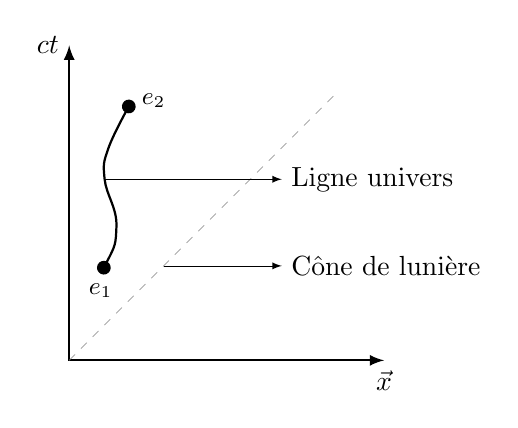
\begin{tikzpicture}
  \draw[thick, latex-latex] (0,4) node[left] {$ct$} -- (0,0) -- (4,0) node[below] {$\vec{x}$};
  \draw[dashed, help lines] (0,0) -- (3.4,3.4);
  \draw [Circle-Circle, thick] plot [smooth, tension=0.7] coordinates {(0.4,1.1) (0.6,1.7) (0.45,2.3) (0.5,2.7) (0.8,3.3)};
  \node [below] at (0.4,1.1) {\small{$e_1$}};
  \node [right] at (0.8,3.3) {\small{$e_2$}};

  \draw [very thin, -latex] (0.45,2.3) -- (2.7,2.3) node [right] {Ligne univers};
  \draw [very thin, -latex] (1.2,1.2) -- (2.7,1.2) node [right] {Cône de lunière};
\end{tikzpicture}

	 \caption{Espace de Minkowski}
 \end{figure}\\
 En reprenant en considération un espace euclidien, on peut donner l'équation du cercle, c'est-à-dire le lieu des points à égale distance d'un point donné : $x^2 + y^2  =  r^2$
 Cette quantité est préservée sous rotation et il donc correct d'écrire, avec R une matrice de rotation:
 \[
	 x^2 +  y^2  \eq
	 \begin{pmatrix}
		 x & y
	 \end{pmatrix}
	 \begin{pmatrix}
		 1 & 0 \\
		 0 & 1 \\
	 \end{pmatrix}
	 \begin{pmatrix}
		 x \\
		 y
	 \end{pmatrix}
	 \eq
	 \begin{pmatrix}
		 x & y
	 \end{pmatrix}
	 R^T
	 \begin{pmatrix}
		 1 & 0 \\
		 0 & 1 \\
	 \end{pmatrix}
	 R
	 \begin{pmatrix}
		 x \\
		 y
	 \end{pmatrix}
 \]
 L'équivalent dans l'espace de Minkowski fait intervenir les transformations de Lorentz\footnote{Qui, pour rappel, peuvent être vues comme l'équivalent d'une rotation mais faisant intervenir le temps (pseudo-rotation). La matrice associée à une pseudo-rotation peut s'écrire comme $L(\xi) = \begin{pmatrix}
	 \cosh(\xi) & \sinh(\xi) \\
	 \sinh(\xi) & \cosh(\xi)
 \end{pmatrix}$} et la matrice $L$:
 \begin{equation}
	 c^2t^2 -  x^2  \eq
	 \begin{pmatrix}
		 ct & x
	 \end{pmatrix}
	 \begin{pmatrix}
		 1 & 0 \\
		 0 & -1 \\
	 \end{pmatrix}
	 \begin{pmatrix}
		 ct \\
		 x
	 \end{pmatrix}
		\eq
	 \begin{pmatrix}
		 ct & x
	 \end{pmatrix}
	 L^T
	 \begin{pmatrix}
		 1 & 0 \\
		 0 & -1 \\
	 \end{pmatrix}
	 L
	 \begin{pmatrix}
		 ct \\
		 x
	 \end{pmatrix}
		\eq
	 \begin{pmatrix}
		 ct' & x'
	 \end{pmatrix}
	 \begin{pmatrix}
		 1 & 0 \\
		 0 & -1 \\
	 \end{pmatrix}
	 \begin{pmatrix}
		 ct' \\
		 x'
	 \end{pmatrix}
 \end{equation}
 Le <<$-$>> dans la matrice centrale vient directement du fait que la métrique n'est pas euclidienne : les dimensions spatiales sont accompagnées d'un <<$-$>> dans la métrique de Minkowski. \textbf{La quantité $c^2t^2 - x^2 = \pm \rho^2$ est ainsi invariante sous les transformations de Lorentz}. Plus précisément, il s'agit de l'équation d'une hyperbole dont les asymptotes sont les lignes de propagation de la lumière.

 \begin{figure}[!ht]
	 \centering
	 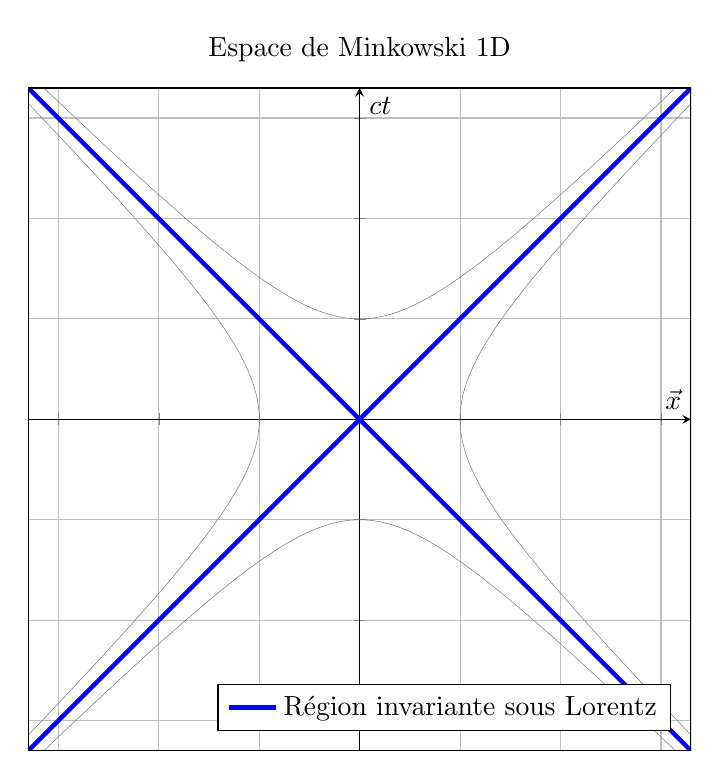
\begin{tikzpicture}
  \begin{axis}[
      samples=121, %nbre de points dans courbes parametrees
      xmin=-3,
      xmax=3,
      ymin=-3,
      ymax=3,
      width=10cm, %taille de la figure
      height=10cm,
      disabledatascaling,
      grid=both, %afficher la grille
      %font=\footnotesize, %taille de la police par defaut
      %grid style={line width=.1pt, draw=red},
      %major grid style={line width=.2pt,draw=gray!50},
      %minor tick num=1,
      axis lines=middle,enlargelimits=0.05, %rendre le plot un rien plus grand
      %execute at begin axis={
      execute at end axis={ %cadre autour
        \draw[thick] (rel axis cs:0,0) -- (rel axis cs:1,0) -- (rel axis cs:1,1) -- (rel axis cs:0,1) --cycle;},
      xticklabels={}, %masquer les nombres en x
      yticklabels={},
      ylabel={$ct$},
      xlabel={$\vec{x}$},
      title={Espace de Minkowski $1$D},
      legend pos=south east,
    ]

    \addplot[ultra thick, blue] expression {x};
    \addplot[ultra thick, blue] expression {-x};
    \legend{Région invariante sous Lorentz}

    \addplot [help lines, domain=-1.9:1.9] ({cosh(x)}, {sinh(x)});
    \addplot [help lines, domain=-1.9:1.9] ({-cosh(x)}, {sinh(x)});
    \addplot [help lines, domain=-1.9:1.9] ({sinh(x)}, {cosh(x)});
    \addplot [help lines, domain=-1.9:1.9] ({sinh(x)}, {-cosh(x)});
  \end{axis}
\end{tikzpicture}

	 \caption{Représentation d'un espace de Minkowski 2D avec la \textbf{région} invariante sous Lorentz.}
 \end{figure}

Le signe de $\rho$ définit sur quelle hyperbole l'objet se situe. Physiquement parlant, les régions latérales sont inaccessibles car savoir quelque chose au sujet d'un événement qui s'y passe impliquerait que l'information en question voyage plus vite que la lumière et la physique possible a donc bien lieu dans les hyperboles supérieures et inférieures (donc $\rho$ est accompagné d'un signe <<$-$>>).

 Quand aux hyperboles latérales, elles ne sont pas physiquement accessible par un quelconque objet se trouvant en (0,0) mais cela ne veut pas dire pour autant qu'elles n'ont aucun sens physique. Ceci prendra sens au point \eqref{contract}.

 \subsection{Extension aux dimensions supérieures et cône de lumière}

		 Les notions abordées précédemment sont toujours valables en 3 et 4D (x,y,z et ct). En ajoutant une dimension, on remarque que les régions de l'espace de Minkowski dans lesquelles se déroulent tous les évènements de la physique sont en réalité deux cônes ; il est impossible de se trouver hors de ces cônes sans aller plus vite que la lumière.
		 \begin{figure}[!ht]
			 \centering
			 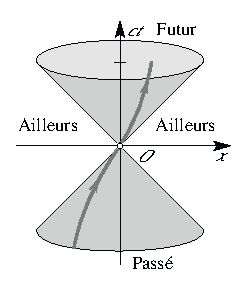
\includegraphics[width=5cm]{Images/minkowski3d.eps}
			 \caption{Représentation d'un espace de Minkowski 3D.}
		 \end{figure}\\
		 La position d'un observateur au repos se situe toujours à l'origine du repère cartésien. Lorsque la vitesse de cet observateur augmente, la
		 position de l'observateur se rapproche des lignes de propagation de la lumière.

 \subsection{Illustrations des concepts de la relativité restreinte par l'espace de Minkowski}

		 Les divers concepts dérivés des transformations de Lorentz peuvent s'illustrer dans l'espace de Minkowski
		 \subsubsection{Simultanéité relative}

			 Il est possible d'utiliser cette représentation pour illustrer l'aspect relatif de la simultanéité, autrement dit la possibilité que deux événements supposés simultanés\footnote{Comprenez: simultanés selon leurs temps propres.} ne le soient plus à cause de la vitesse relative d'un des deux référentiels.

			 \begin{figure}[!ht]
				 \centering
				 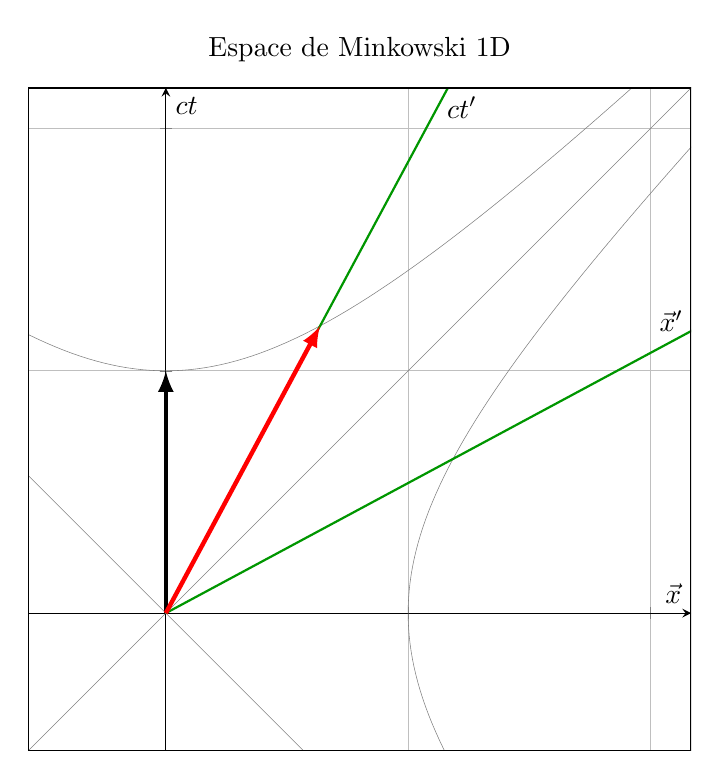
\begin{tikzpicture}
  \begin{axis}[
      samples=121,
      xmin=-0.4,
      xmax=2.,
      ymin=-0.4,
      ymax=2.,
      width=10cm,
      height=10cm,
      grid=both,
      disabledatascaling,
      %font=\footnotesize,
      %grid style={line width=.1pt, draw=red},
      %major grid style={line width=.2pt,draw=gray!50},
      %minor tick num=1,
      axis lines=middle,enlargelimits=0.07,
      %execute at begin axis={
      execute at end axis={
        \draw[thick] (rel axis cs:0,0) -- (rel axis cs:1,0) -- (rel axis cs:1,1) -- (rel axis cs:0,1) --cycle;},
      xticklabels={},
      yticklabels={},
      xtick={-10,-9,...,10},
      ytick={-10,-9,...,10},
      ylabel={$ct$},
      xlabel={$\vec{x}$},
      title={Espace de Minkowski $1$D},
      legend pos=south east,
    ]

    \addplot[help lines] expression {x};
    \addplot[help lines] expression {-x};

    \addplot [help lines, domain=-1.9:1.9] ({cosh(x)}, {sinh(x)});
    \addplot [help lines, domain=-1.9:1.9] ({-cosh(x)}, {sinh(x)});
    \addplot [help lines, domain=-1.9:1.9] ({sinh(x)}, {cosh(x)});
    \addplot [help lines, domain=-1.9:1.9] ({sinh(x)}, {-cosh(x)});
    %\addlegendentry{$x^2$}

    \pgfmathsetmacro{\i}{sinh(0.6)}
    \pgfmathsetmacro{\j}{cosh(0.6)}

    \draw [dgreen, thick] (axis cs:0,0) -- (axis cs:2*\i,2*\j);
    \draw [dgreen, thick] (axis cs:0,0) -- (axis cs:2*\j,2*\i);

    \draw[ultra thick, -latex] (axis cs:0,0) -- (axis cs:0,1);
    \draw[ultra thick, -latex, red] (axis cs:0,0) -- (axis cs:\i,\j);

    \node [right] at (axis cs:1.76*\i, 1.76*\j) {$ct'$};
    \node [above] at (axis cs:1.76*\j, 1.76*\i) {$\vec{x}'$};

    %\pgfmathparse{10*0.05}
  \end{axis}
\end{tikzpicture}

				 \caption{Représentation des axes $ct$ et $x$ de deux référentiels, l'un en MRU l'autre au repos.}
				 \label{mink}
			 \end{figure}

			 En prenant la projection du vecteur rouge sur l'axe ct, on remarque effectivement les deux événements ne sont pas simultanés entre les deux référentiels. La notion de simultanéité est donc à mettre en relation avec les coordonnées spatiales. On dit donc de deux événements qu'ils sont simultanés s'ils le sont effectivement quand leurs référentiels coïncident. Autrement dit, si les deux évenements se placent sur une même hyperbole, c'est-à-dire si la quantité $c\tau^2$ est identique pour chacun.

		 \subsubsection{Dilatation du temps}

			 La figure \eqref{mink} permet de se rendre compte du phénomène de dilatation du temps. De prime abord, il est aisé de remarquer que la projection du vecteur du référentiel $(x',ct')$ sur l'axe $ct$ du référentiel $(x,ct)$ est plus grande que le vecteur du référentiel $(x,ct)$. Or, ces deux vecteurs ont un temps propre identique (ils pointent la même hyperbole). Par conséquent, une seconde pour l'observateur au repos (référentiel $(x,ct)$) paraît plus courte que pour l'observateur en mouvement (référentiel $(x',ct')$).

			 Plus précisément, il est possible de retrouver la dilatation du temps : $t = \gamma \tau$ avec $\tau$ le temps propre. Considérons la figure \eqref{MinkTemps} : deux évènements ($e'_1$ et $e'_2$) ont lieux en des instants différents dans les deux référentiels et se trouvent au même point de l'espace dans $\mathcal{R'}$.
				\begin{figure}[!ht]
				 \centering
				 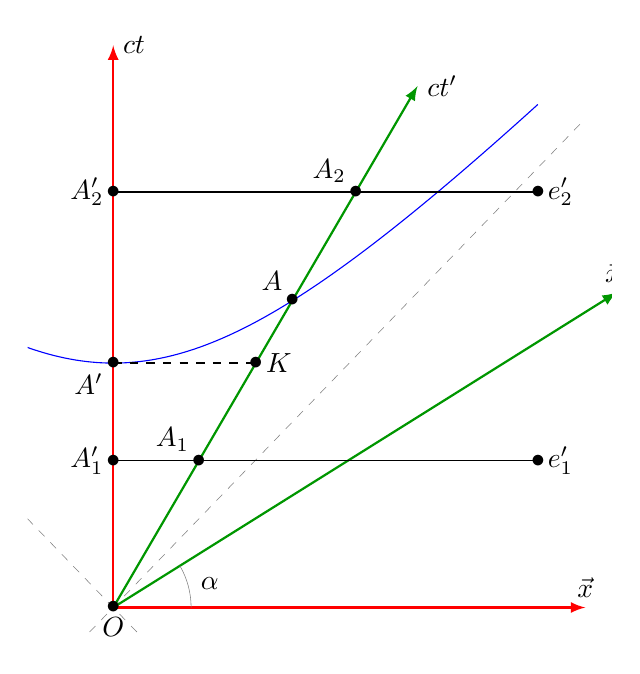
\begin{tikzpicture}
  \begin{axis}[
      samples=121,
      xmin=-.25,
      xmax=2.,
      ymin=-0.2,
      ymax=2.5,
      width=9cm,
      height=10.8cm,
      disabledatascaling,
      %grid=both,
      %font=\footnotesize,
      %grid style={line width=.1pt, draw=red},
      %major grid style={line width=.2pt,draw=gray!50},
      %minor tick num=1,
      axis lines=none,enlargelimits=0.05,
      %execute at begin axis={
      %execute at end axis={        \draw[thick] (rel axis cs:0,0) -- (rel axis cs:1,0) -- (rel axis cs:1,1) -- (rel axis cs:0,1) --cycle;},
      xticklabels={},
      yticklabels={},
      xtick={-10,-9,...,10},
      ytick={-10,-9,...,10},
      ylabel={$ct$},
      xlabel={$\vec{x}$},
      %title={Espace de Minkowski $1$D},
      legend pos=south east,
    ]

    \addplot [color=blue, domain=-1.35:1.35] ({sinh(x)}, {cosh(x)});
    %\addlegendentry{$x^2$}

    \pgfmathsetmacro{\i}{sinh(0.7)}
    \pgfmathsetmacro{\j}{cosh(0.7)}
    \pgfmathsetmacro{\alxi}{atan(tanh(0.7))}

    \draw [dashed, help lines] (0.1,-0.1) -- (-2,2) (-0.1,-0.1) -- (2,2);
    \draw [red, thick, latex-latex] (0,2.3) -- (0,0) -- (2,0);
    \draw [dgreen, thick, -latex] (0,0) -- (1.7*\i,1.7*\j);
    \draw [dgreen, thick, -latex] (0,0) -- (1.7*\j,1.7*\i);


    \node [right] at (1.7*\i, 1.7*\j) {$ct'$};
    \node [above] at (1.7*\j, 1.7*\i) {$\vec{x}'$};
    \node [right] at (0,2.3) {$ct$};
    \node [above] at (2,0) {$\vec{x}$};

    \draw [dashed, thick] (0,1) node {$\bullet$} node [below left] {$A'$} -- (\i/\j,1) node {$\bullet$} node [right] {$K$};
    \draw (0,.6) node {$\bullet$} node [left] {$A_1'$} -- (0.6*\i/\j,.6) node {$\bullet$} node [above left] {$A_1$} -- (1.8,0.6) node {$\bullet$} node [right] {$e_1'$};
    \draw (0,1.7) node {$\bullet$} node [left] {$A_2'$} -- (1.7*\i/\j,1.7) node {$\bullet$} node [above left] {$A_2$} -- (1.8,1.7) node {$\bullet$} node [right] {$e_2'$};

    \draw [help lines] (0.33,0) arc (0:\alxi:0.33);
    \node [right] at (0.33,0.1) {$\alpha$};
    \draw (0,0) node [below] {$O$} node {$\bullet$};
    \draw (\i,\j) node [above left] {$A$} node {$\bullet$};

    %\pgfmathparse{10*0.05}
  \end{axis}
\end{tikzpicture}

				 \caption{Visualisation de la dilatation du temps dans un diagramme de Minkowski}
				 \label{MinkTemps}
			 \end{figure}\\
			 L'intersection de l'hyperbole avec les axes $ct$ et $ct'$ représente l'unité dans chacun des deux référentiels. De plus, l'invariant $ds$ mène à la relation suivante :
			 \[
				 ds^2 \eq c^2 dt^2 - dx^2 \eq c^2 dt'^2 - dx'^2 = +1 \quad \textrm{(<<$+$>> car on se trouve sur l'hyperbole du dessus)}
			 \]
			 Par conséquent :
			 \begin{itemize}
				 \item si $dx=0$, on se trouve sur $ct$ et \quad $c \cdot dt = 1$
				 \item si $dx'=0$, on se trouve sur $ct'$ et \quad $c \cdot dt' = 1$
			 \end{itemize}
			 Dénommons $OA$ l'unité dans $\mathcal{R}$ et $OA'$ l'unité dans $\mathcal{R'}$. Il est à noter que $OA$ et $OA'$ sont des longueurs symbolisant des durées. Il est ainsi possible d'exprimer les temps propre ($T_p$) et impropre ($T_i$) séparant les deux évènements :
			 \[
				 \boxed{T_p \eq \dfrac{A_1A_2}{OA}}
					 \qquad \textrm{et} \qquad
				 \boxed{T_i \eq \dfrac{A'_1A'_2}{OA'}}
			 \]
			 Le but va de maintenant trouver une relation entre $T_p$ et $T_i$. La trigonométrie sur la figure \eqref{MinkTemps} permet de dériver l'expression suivante :
			 \[
				 \cos(\alpha) \eq \dfrac{OA'}{OK} \eq \dfrac{A'_1A'_2}{A_1A_2}
				 \quad \Leftrightarrow \quad
				 \dfrac{A'_1A'_2}{OA'} \eq \dfrac{OA}{OK} \cdot \dfrac{A_1A_2}{OA}
				 \quad \Leftrightarrow \quad
				 \boxed{T_i \eq \dfrac{OA}{OK} T_p}
			 \]
			 Pour obtenir la relation finale reliant $T_i$ et $T_p$, il faut déterminer ce que vaut le rapport entre $OA$ et $OK$. Pour ce faire, chacune des deux longueurs va être exprimée en terme de $OA'$:
			 \begin{enumerate}

				 \item En prenant le triangle formé par les axes $ct'$ et $ct$ et en fixant un point quelconque $(ct,x)$, il est possible de dériver que $tg(\alpha) = \dfrac{dx'}{cdt'} = v'/c = \beta$.

				 En utilisant certaines identités trigonométriques, il est possible d'exprimer une relation entre $OK$ et $OA'$:
				 \begin{align}
					 \cos^2\alpha + \sin^2\alpha = 1
						 &\Leftrightarrow \quad
					 1 + tg^2\alpha \eq \dfrac{1}{\cos^2\alpha}
						 \\[7pt]
						 &\Leftrightarrow \quad
					 1 + \beta^2 \eq \left( \dfrac{OK}{OA'} \right)^2
						 \\[7pt]
						 &\Leftrightarrow \quad
					 \boxed{OK \eq OA' \cdot \sqrt{1+\beta^2}}
				 \end{align}

				 \item $A'$ étant l'intersection entre l'hyperbole et l'axe $ct'$, il est possible de de trouver l'expression suivante:
				 \[
					 (OA')^2 \eq ds^2 \eq c^2 dt'^2 - dx'^2
					 \quad \Leftrightarrow \quad
					 OA' \eq \sqrt{c^2 dt'^2 - dx'^2}
				 \]
				 Or, $dx' \eq v \cdot dt' \quad \Leftrightarrow \quad dx' \eq \beta \cdot c\cdot dt'$. Par conséquent,
				 \[
					 OA' \eq
					 \sqrt{c^2 dt'^2 - \beta^2 c^2dt'^2} \eq
					 c\cdot dt' \cdot \sqrt{1 - \beta^2}
				 \]
				 Par Pythagore, $OA \eq \sqrt{c^2 dt'^2 + dx'^2} \eq \sqrt{c^2 dt'^2 + \beta^2 c^2dt'^2} \eq c\cdot dt' \cdot \sqrt{1 + \beta^2}$.

				 En faisant le rapport entre $OA$ et $OA'$, l'expression suivante est obtenue:
				 \[
					 \dfrac{OA}{OA'} \eq
					 \dfrac{ c\cdot dt' \cdot \sqrt{1 + \beta^2}}{ c\cdot dt' \cdot \sqrt{1 - \beta^2}}
					 \quad \Leftrightarrow \quad
					 \boxed{
						 OA \eq OA' \cdot \sqrt{   \dfrac{1 + \beta^2}{1 - \beta^2}  }
					 }
				 \]
			 \end{enumerate}
			 Il est maintenant possible d'exprimer le rapport en $OA$ et $OK$, rapport reliant le temps propre et le temps impropre:
			 \[
				 \dfrac{OA}{OK} \eq
				 \dfrac{OA' \cdot \sqrt{\dfrac{1 + \beta^2}{1 - \beta^2}}}{OA' \cdot \sqrt{1+\beta^2}}
				 \eq \gamma
				 \quad \Leftrightarrow \quad
				 \boxed{ T_i \eq \gamma T_p }
			 \]

		 \subsubsection{Contraction des longueurs} \label{contract}

			 La contraction des longueurs peut être également traduite dans l'espace de Minkowski. Supposons que nous disposions d'un train d'une certaine longueur dans son référentiel propre $(x,ct)$. Supposons également un observateur dans un référentiel $(x',ct')$ en mouvement par rapport au référentiel propre du train.

			 Pour l'observateur en mouvement par rapport au train, la longueur <<1>> est celle ayant suivi la courbe d'hyperbole. Par conséquent, son unité de mesure est visiblement plus grande que l'unité de mesure dans le référentiel propre au train. Si l'observateur en MRU essaye maintenant de mesurer le train avec son unité de mesure, il aura besoin de moins d'unités de longueurs pour mesurer le train. Par conséquent, le train lui apparaît plus petit.

			 On a donc bien contraction des longueurs du point de vue du référentiel en mouvement.
			 \begin{figure}[!ht]
				 \centering
				 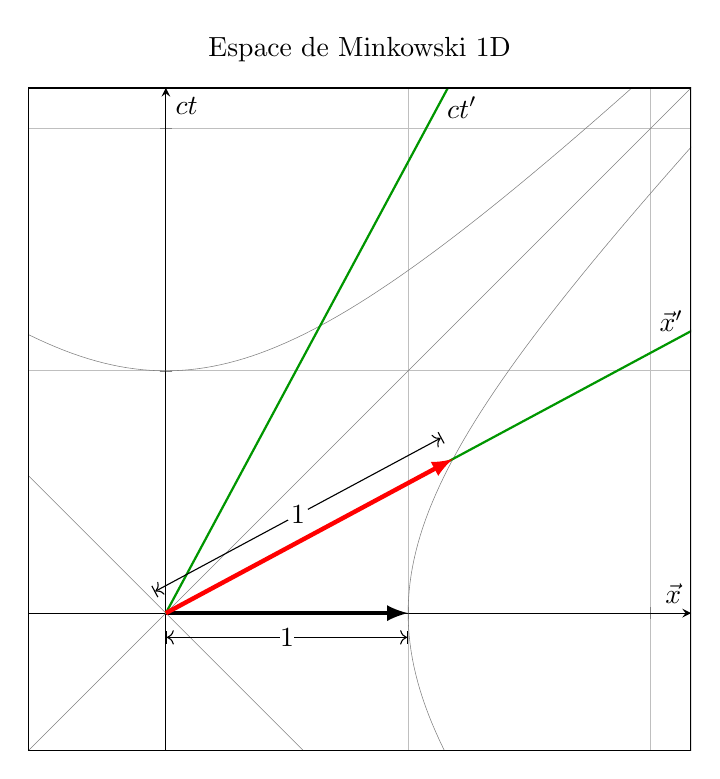
\begin{tikzpicture}
  \begin{axis}[
      samples=121,
      xmin=-0.4,
      xmax=2.,
      ymin=-0.4,
      ymax=2.,
      width=10cm,
      height=10cm,
      grid=both,
      disabledatascaling,
      %font=\footnotesize,
      %grid style={line width=.1pt, draw=red},
      %major grid style={line width=.2pt,draw=gray!50},
      %minor tick num=1,
      axis lines=middle,enlargelimits=0.07,
      %execute at begin axis={
      execute at end axis={
        \draw[thick] (rel axis cs:0,0) -- (rel axis cs:1,0) -- (rel axis cs:1,1) -- (rel axis cs:0,1) --cycle;},
      xticklabels={},
      yticklabels={},
      xtick={-10,-9,...,10},
      ytick={-10,-9,...,10},
      ylabel={$ct$},
      xlabel={$\vec{x}$},
      title={Espace de Minkowski $1$D},
      legend pos=south east,
    ]

    \addplot[help lines] expression {x};
    \addplot[help lines] expression {-x};

    \addplot [help lines, domain=-1.9:1.9] ({cosh(x)}, {sinh(x)});
    \addplot [help lines, domain=-1.9:1.9] ({-cosh(x)}, {sinh(x)});
    \addplot [help lines, domain=-1.9:1.9] ({sinh(x)}, {cosh(x)});
    \addplot [help lines, domain=-1.9:1.9] ({sinh(x)}, {-cosh(x)});
    %\addlegendentry{$x^2$}

    \pgfmathsetmacro{\i}{sinh(0.6)}
    \pgfmathsetmacro{\j}{cosh(0.6)}
    \pgfmathsetmacro{\d}{sqrt(\i^2 + \j^2)}
    \pgfmathsetmacro{\alxi}{atan(tanh(0.6))}

    \draw [dgreen, thick] (0,0) -- (2*\i,2*\j);
    \draw [dgreen, thick] (0,0) -- (2*\j,2*\i);

    \draw[ultra thick, -latex] (0,0) -- (.5,0) -- (1,0);
    \draw[thin, |<->|] (0,-.1) -- (.5,-.1) node[fill=white, inner sep=0pt] {1} -- (1,-.1);

    \draw[ultra thick, -latex, red] (0,0) -- (0.5*\j,0.5*\i) -- (\j,\i);
    \draw[thin, rotate=\alxi, |<->|] (0,.1) -- (.5*\d,.1) node[circle, fill=white, inner sep=0pt] {1} -- (\d,.1);

    \node [right] at (1.76*\i, 1.76*\j) {$ct'$};
    \node [above] at (1.76*\j, 1.76*\i) {$\vec{x}'$};

    %\pgfmathparse{10*0.05}
  \end{axis}
\end{tikzpicture}

				 \caption{Représentation des axes $ct$ et $x$ de deux référentiels, l'un en MRU l'autre au repos.}
			 \end{figure}
			 De façon plus qualitative, l'expression de la contraction des longueurs peut être dérivée de façon similaire à la dilatation du temps. En considérant la figure \eqref{MinkLong}
			 \begin{figure}[!ht]
				 \centering
				 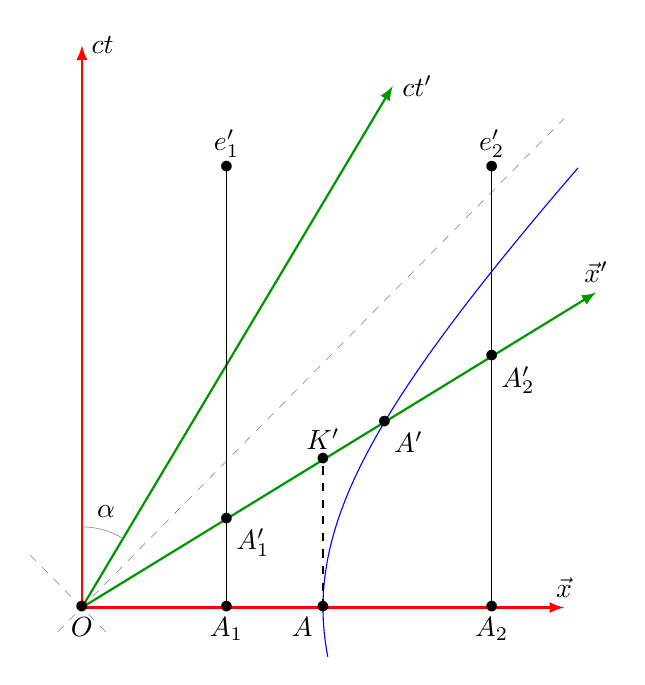
\begin{tikzpicture}
  \begin{axis}[
      samples=121,
      xmin=-0.1,
      xmax=2.4,
      ymin=-0.3,
      ymax=2.4,
      width=10cm,
      height=10.8cm,
      disabledatascaling,
      %grid=both,
      %font=\footnotesize,
      %grid style={line width=.1pt, draw=red},
      %major grid style={line width=.2pt,draw=gray!50},
      %minor tick num=1,
      axis lines=none,enlargelimits=0.05,
      %execute at begin axis={
      %execute at end axis={        \draw[thick] (rel axis cs:0,0) -- (rel axis cs:1,0) -- (rel axis cs:1,1) -- (rel axis cs:0,1) --cycle;},
      xticklabels={},
      yticklabels={},
      xtick={-10,-9,...,10},
      ytick={-10,-9,...,10},
      ylabel={$ct$},
      xlabel={$\vec{x}$},
      %title={Espace de Minkowski $1$D},
      legend pos=south east,
    ]

    \addplot [color=blue, domain=-0.2:1.35] ({cosh(x)}, {sinh(x)});
    %\addlegendentry{$x^2$}

    \pgfmathsetmacro{\i}{sinh(0.7)}
    \pgfmathsetmacro{\j}{cosh(0.7)}
    \pgfmathsetmacro{\alxi}{atan(tanh(0.7))}

    \draw [dashed, help lines] (0.1,-0.1) -- (-2,2) (-0.1,-0.1) -- (2,2);
    \draw [red, thick, latex-latex] (0,2.3) -- (0,0) -- (2,0);
    \draw [dgreen, thick, -latex] (0,0) -- (1.7*\i,1.7*\j);
    \draw [dgreen, thick, -latex] (0,0) -- (1.7*\j,1.7*\i);


    \node [right] at (1.7*\i, 1.7*\j) {$ct'$};
    \node [above] at (1.7*\j, 1.7*\i) {$\vec{x}'$};
    \node [right] at (0,2.3) {$ct$};
    \node [above] at (2,0) {$\vec{x}$};

    \draw (.6,0) node {$\bullet$} node [below] {$A_1$} -- (.6,0.6*\i/\j) node {$\bullet$} node [below right] {$A_1'$} -- (.6,1.8) node {$\bullet$} node [above] {$e_1'$};

    \draw [dashed, thick] (1,0) node {$\bullet$} node [below left] {$A$} -- (1,\i/\j) node {$\bullet$} node [above] {$K'$};

    \draw (1.7,0) node {$\bullet$} node [below] {$A_2$} -- (1.7,1.7*\i/\j) node {$\bullet$} node [below right] {$A_2'$} -- (1.7,1.8) node {$\bullet$} node [above] {$e_2'$};

    \draw [help lines] (0,0.33) arc (90:90-\alxi:0.33);
    \node [above] at (0.1,0.33) {$\alpha$};
    \draw (0,0) node [below] {$O$} node {$\bullet$};
    \draw (\j,\i) node [below right] {$A'$} node {$\bullet$};

  \end{axis}
\end{tikzpicture}

				 \caption{Visualisation de la contraction des longueurs dans un diagramme de Minkowski}
				 \label{MinkLong}
			 \end{figure}
			 Il est ainsi possible de retrouver la contraction des longueurs : $L_i = \gamma^{-1} L_p$. Soit un objet immobile dans $\mathcal{R}$ de longueur propre $L_p$. Que vaut cette longueur pour un observateur se situant dans $\mathcal{R'}$?\\
			 L'intersection de l'hyperbole avec les axes $x$ et $x'$ représente l'unité dans chacun des deux référentiels. De plus, l'invariant $ds$ mène à la relation suivante :
			 \[
				 - ds^2 \eq c^2 dt^2 - dx^2 \eq c^2 dt'^2 - dx'^2 = -1 \quad \textrm{(<<$-$>> car on se trouve sur l'hyperbole du dessus)}
			 \]
			 Par conséquent :
			 \begin{itemize}
				 \item si $c\cdot dt=0$,   on se trouve sur $x$  et \quad $dx = 1$
				 \item si $c \cdot dt'=0$, on se trouve sur $x'$ et \quad $dx' = 1$
			 \end{itemize}
			 Dénommons $OA$ l'unité dans $\mathcal{R}$ et $OA'$ l'unité dans $\mathcal{R'}$. Il est ainsi possible d'exprimer les longueurs propre ($L_p$) et impropre ($L_i$) séparant les deux évènements :
			 \[
				 \boxed{L_p \eq \dfrac{A_1A_2}{OA}}
					 \qquad \textrm{et} \qquad
				 \boxed{L_i \eq \dfrac{A'_1A'_2}{OA'}}
			 \]
			 Le but va de maintenant trouver une relation entre $L_p$ et $L_i$. La trigonométrie sur la figure \eqref{MinkTemps} permet de dériver l'expression suivante :
			 \[
				 \cos(\alpha) \eq \dfrac{OA}{OK'} \eq \dfrac{A_1A_2}{A'_1A'_2}
				 \quad \Leftrightarrow \quad
				 \dfrac{A_1A_2}{OA} \eq \dfrac{OA'}{OK'} \cdot \dfrac{A'_1A'_2}{OA'}
				 \quad \Leftrightarrow \quad
				 \boxed{L_i \eq \dfrac{OK'}{OA'} L_p}
			 \]
			 Pour obtenir la relation finale reliant $L_i$ et $L_p$, il faut déterminer ce que vaut le rapport entre $OK'$ et $OA'$. Pour ce faire, chacune des deux longueurs va être exprimée en terme de $OA$:
			 \begin{enumerate}
				 \item En prenant le triangle formé par les axes $x'$ et $x$ et en fixant un point quelconque $(ct,x)$, il est possible de dériver que $tg(\alpha) = \dfrac{dx'}{cdt'} = v'/c = \beta$.

				 En utilisant certaines identités trigonométriques, il est possible d'exprimer une relation entre $OK$ et $OA'$:
				 \begin{align}
					 \cos^2\alpha + \sin^2\alpha = 1
						 &\Leftrightarrow \quad
					 1 + tg^2\alpha \eq \dfrac{1}{\cos^2\alpha}\\[7pt]
						 &\Leftrightarrow \quad
					 1 + \beta^2 \eq \left( \dfrac{OK'}{OA} \right)^2\\[7pt]
						 &\Leftrightarrow \quad
					 \boxed{OK' \eq OA \cdot \sqrt{1+\beta^2}}
				 \end{align}
				 \item $A'$ étant l'intersection entre l'hyperbole et l'axe $x'$, il est possible de trouver l'expression suivante:

				 \[
					 -(OA)^2 \eq - ds^2 \eq c^2 dt^2 - dx^2
					 \quad \Leftrightarrow \quad
					 OA \eq \sqrt{dx^2 - c^2 dt^2}
				 \]
				 En utilisant les transformations de Lorentz (il doit exister une autre façon de dériver cette expression mais elle n'a pas encore été trouvée), et en imposant que $c \cdot dt' = 0$, la relation $ct = \beta x$ est obtenue. Par conséquent:
				 \[
					 OA \eq
					 \sqrt{dx^2 - \beta^2 dx^2} \eq
					 dx \cdot \sqrt{1 - \beta^2}
				 \]

				 Par Pythagore, $OA' \eq \sqrt{c^2 dt^2 + dx^2} \eq \sqrt{\beta^2 dx^2 + dx^2} \eq dx \cdot \sqrt{\beta^2 + 1}$.

				 En faisant le rapport entre $OA$ et $OA'$, l'expression suivante est obtenue:
				 \[
					 \dfrac{OA}{OA'} \eq
					 \dfrac{ dx \cdot \sqrt{1 - \beta^2} }{ dx \cdot \sqrt{\beta^2 + 1} }
					 \quad \Leftrightarrow \quad
					 \boxed{
						 OA \eq OA' \cdot \sqrt{   \dfrac{1 - \beta^2}{1 + \beta^2}  }
					 }
				 \]
			 \end{enumerate}
			 Il est maintenant possible d'exprimer le rapport en $OA'$ et $OK'$, rapport reliant la longueur propre et la longueur impropre:
			 \[
				 \dfrac{OA'}{OK'} \eq
				 \dfrac{OA' \cdot \sqrt{   \dfrac{1 - \beta^2}{1 + \beta^2}  }}{OA \cdot \sqrt{1+\beta^2}}
				 \eq \gamma^{-1}
				 \quad \Leftrightarrow \quad
				 \boxed{ L_i \eq \gamma^{-1} L_p }
			 \]
\newpage

\section{Cinématique relativiste}
\subsection{Le quadrivecteur de position}

	Il est possible de définir l'intervalle de temps-espace: la modification infinitésimale dans l'espace temps. Il s'agit d'un quadri-vecteur. Plus précisément, il s'agit uniquement d'adjoindre le temps au vecteur 3x1 habituel des 3 dimensions de l'espace.
	\begin{equation}
		\boxed{   dx^\mu   \eqq     (c \cdot dt \; , \; d\vec{x})    \eqq    (c \cdot dt \; , \; dx \; , \; dy \; , \; dz)  }
	\end{equation}
	Par convention, les lettres grecques dénotent les indices utilisés pour le temps et l'espace (il s'agira du cas le plus fréquent dans la suite de notre discussion) tandis que les lettres latines dénotent les dimensions d'espace seules.
	\[
		\alpha, \beta, \gamma ... \longrightarrow (0,1,2,3)
	\]
	\[
		a, b, c ... \longrightarrow (1,2,3)
	\]
	Cette notation introduite, nous pouvons développer l'invariant pour les transformations de Lorentz trouvé au point précédent.
	\begin{equation}
		\boxed{
			ds^2 \eq c^2dt^2 - d\vec{x} \cdot d\vec{x} \eq \eta_{\mu \nu} dx^\mu dx^\nu \eq c^2 d\tau^2
		}
	\end{equation}
	\begin{equation}
		\boxed{
			\eta_{\mu \nu} \eq \begin{pmatrix}
				1&0&0&0\\
				0&-1&0&0\\
				0&0&-1&0\\
				0&0&0&-1\\
			\end{pmatrix}
		}
	\end{equation}
	A ce stade, il est très important de remarquer plusieurs choses:
	\begin{enumerate}
		\item En se rappelant la convention d'Einstein, il est évident que $\eta_{\mu \nu} dx^\mu dx^\nu$ est une double somme de termes allant des indices 0 à 3.
		\item Bien qu'on écrive $dx^\mu$ la lettre grecque nous indique bien que ce vecteur comprend espace et temps et que donc pour $\mu = 0$ ou $\nu = 0$ on fait bien référence à la composante temporelle du quadri-vecteur $dx^\mu$.
		\item $c^2d\tau^2$ est bien l'invariant que nous cherchions, il fait intervenir le temps propre.
		\item La matrice $\eta_{\mu \nu}$ définit implicitement un nouveau produit scalaire et par conséquent une nouvelle norme différente de celle d'un espace classique. On peut donc écrire pour une ligne d'Univers reliant deux événements quelconques $E_1$ et $E_2$  : $|E_1E_2| \eq c^2(t_2-t_1)^2 - (x_2 - x_1)^2$
	\end{enumerate}
	Ces notions doivent vous permettre de mieux appréhender l'explication de la durée de vie <<allongée>> des muons cosmiques reprise au point \ref{Muons}.

\subsection{Le quadrivecteur vitesse}

		Cette section est exclusivement tirée du livre et n'a donc pas été décrite lors des cours magistraux. Cependant, elle permet une meilleure compréhension de la cinématique relativiste et permet de réutiliser et redériver des expressions connues.

	\subsubsection{Définition et formule de transformation}

		En relativité restreinte, le 3-vecteur vitesse $\vec{v}$ devient le 4-vecteur vitesse relativiste $u^\mu$. il se définit comme la dérivée selon le temps propre $\tau$ du 4-vecteur position défini précédemment.
		\begin{align}
			\boxed{u^\mu \eq \dfrac{dx^\mu}{d\tau}}
		\end{align}
		Rappelons également le lien entre temps propre $d\tau$ et impropre $dt$ :
		\begin{align}
			\boxed{d\tau = \gamma^{-1}dt}
		\end{align}
		Plaçons-nous à nouveau dans un espace à deux dimensions $x$ et $t$ dans lequel se trouvent deux référentiels $\mathcal{R}$ et $\mathcal{R'}$ respectivement eu repos et se déplaçant à une vitesse $v_e$. Par transformation de Lorentz :
		\begin{align}
			\left\{
				\begin{array}{ll}
					ct \eq \gamma_e (ct' + \beta_e x')\\
					x \eq \gamma_e (x + \beta_e ct')
				\end{array}
			\right.
		\end{align}
		En différenciant ces relations ($v_e$ est constant) on obtient :
		\begin{align}
			\left\{
				\begin{array}{ll}
					cdt \eq \gamma_e (cdt' + \beta_e dx')\\
					dx \eq \gamma_e (dx + \beta_e cdt')
				\end{array}
			\right.
		\end{align}
		Enfin, l'\textbf{addition relativiste} des vitesses peut être redérivée en prenant le rapport des deux équations ci-dessus puis en simplifiant numérateur et dénominateur par $dt'$. Cette dernière étape permet l'apparition de la vitesse $v' = \dfrac{dx'}{dt'}$.
		\begin{align}
			\dfrac{dx}{cdt}
		\eq
			\dfrac{\gamma_e (dx + \beta_e cdt')}{\gamma_e (cdt' + \beta_e dx')}
		\eq
			\dfrac{dx + \beta_e cdt'}{cdt' + \beta_e dx'}
		\eq
			\dfrac{dx/dt' \;+\; \beta_e}{c \;+\; \beta_e dx'/dt'}
		\quad \Leftrightarrow \quad
			\dfrac{dx}{dt}
		\eq
			\boxed{
				v \eq \dfrac{v' + v_e}{1 + \dfrac{v_ev'}{c^2}}
			}
		\end{align}
		Cette expression avait déjà été dérivée dans la section \ref{verif} avec une vision axée sur l'application linéaire de pseudo-rotation $L(\xi)$.

	\subsubsection{Norme du 4-vecteur vitesse}

		La norme du 4-vecteur vitesse peut être facilement établie:
		\begin{align}
			\eta_{\mu\nu}u^\mu u^\nu
				&= \; \gamma^2c^2 - \gamma^2|\vec{v}|^2\\[7pt]
				&= \; \gamma^2(c^2 - |\vec{v}|^2)\\[7pt]
				&= \; c^2
		\end{align}
		Le caractère constant de la norme du 4-vecteur vitesse nous servira pour établir l'orthogonalité des vecteurs vitesse $u^\mu$ et accélération $\omega^\mu$.

	\subsubsection{Rapidité}

		En relativité, les vitesses ne sont plus additives, cependant il est possible de définir une nouvelle grandeur analogue qui elle l'est : la rapidité. Son expression pour une vitesse orientée exclusivement selon l'axe x est:
		\begin{align}
			\tanh(r_x)
				&\overset{\Delta}{\eq}
					\dfrac{v_x}{c}\\[7pt]
				&\eq
					\dfrac{\tanh(r_x') + \tanh(r_e)}{1 + \tanh(r_x')\tanh(r_e)}\\[7pt]
				&\eq
					\tanh(r_x' + r_e)
					\quad \Leftrightarrow \quad
					\boxed{r_x \eq r'_x + r_e}
		\end{align}
		En cinématique einsteinienne, ce sont donc les rapidités selon l'axe du mouvement qui s'additionnent et non les vitesses. Cette additivité des rapidités est équivalent à l'additivité galiléennes des vitesses dans un cadre non-relativiste.

\subsection{Le quadrivecteur d'onde}

	Afin d'introduire le 4-vecteur d'onde dans l'espace de Minkowski, il faut considérer une onde plane monochromatique $\nu$, dont l'équation 1D s'écrit comme:
	\begin{equation}
		\psi \eq \psi_0 \cdot \cos(\omega t - \vec{k}\vec{x})
	\end{equation}
	Un telle onde doit satisfaire les équations de Maxwell : $\Box \bar{E} = 0$ et $\Box \bar{B} = 0$ avec le d'alembertien $\Box$:
	\begin{align}
			\Box
				\; &= \;
			\dfrac{1}{c^2}\dfrac{\p^2 }{\p^2t} \, - \, \Delta \\
				&= \;
			\eta_{\mu \nu} \p^\mu \p^\nu
				\quad \textrm{tel que} \quad
			\p^\mu \eq \dfrac{\p}{\p x_\mu}
	\end{align}
	$\phi$ peut donc s'écrire comme:
	\begin{equation}
		\phi   \eq   \phi_0 \cdot \cos(k^\mu x_\mu)   \eq   \phi_0 \cdot \cos(\eta_{\mu\nu}k^\mu x^\mu)
	\end{equation}
	L'équation d'onde étant invariante sous Lorentz, sa solution doit l'être aussi. Par conséquent, $k^\mu x_\mu$ doit être un invariant et pouvoir s'écrire sur la forme suivante:
	\begin{equation}
		k^\mu x_\mu
			\eq
		\eta_{\mu \nu}k^\mu x^\nu
			\quad \textrm{tel que} \quad
		\boxed{
			k^\mu \eq
			\begin{pmatrix}
				\omega/c\\
				\vec{k}
			\end{pmatrix}
			}
	\end{equation}
	Il est très intéressant de noter qu'à nouveau en adjoignant le nombre d'ondes $k$ (qui peut être exprimé comme la fréquence spatiale) à la fréquence temporelle ($\omega = 2\pi \nu$), on lie à nouveau 3 dimensions d'espace et une de temps dans un quadri-vecteur.

	Une des propriétés du quadrivecteur d'onde $k^\mu$ \footnote{Nous vous recommandons d'ailleurs <<La peste>> ou encore <<L'étranger>>.} est que son produit scalaire dans un espace de Minkowski est nul:
	\begin{equation}
		k^2 \eq \eta_{\mu \nu} k^\mu k^\nu \eq 0
	\end{equation}
	\begin{center}
		car $\dfrac{\omega}{c} \eq |\vec{k}|$
	\end{center}

	\subsubsection{Applications}

		\paragraph{L'effet Doppler-Fizeau}

			\begin{figure}[!ht]
				\centering
				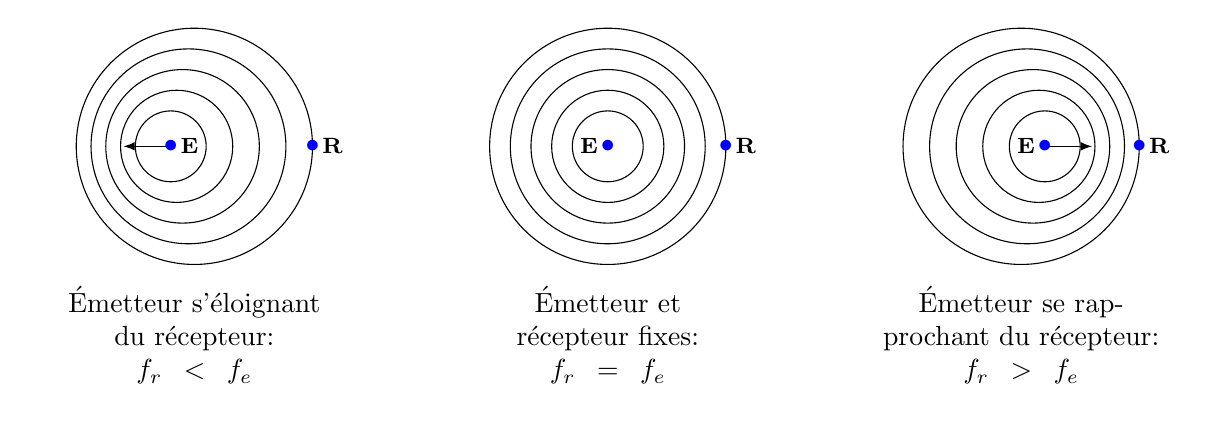
\begin{tikzpicture}[scale=0.75]
  \begin{scope}[shift={(-7,0)}]
    \foreach \i in {0,...,4}{
      \draw (-\i*0.1,0) circle[radius=2-\i*0.35];}

    \draw[-latex] (-.4,0) node[blue]  {$\bullet$} node[right] {\footnotesize{\textbf{E}}} --++(-0.8,0);
    \draw (2,0) node[blue]  {$\bullet$} node[right] {\footnotesize{\textbf{R}}};
    \node[text width=4cm,align=center] at (0,-3.2) {Émetteur s'éloignant du récepteur:\\ $f_r < f_e$};
  \end{scope}

  \begin{scope}
    \foreach \i in {0,...,4}{
      \draw (0,0) circle[radius=2-\i*0.35];}

    \draw (0,0) node[blue]  {$\bullet$} node[left] {\footnotesize{\textbf{E}}};
    \draw (2,0) node[blue]  {$\bullet$} node[right] {\footnotesize{\textbf{R}}};
    \node[text width=4cm,align=center] at (0,-3.2) {Émetteur et récepteur fixes:\\ $f_r = f_e$};
  \end{scope}

  \begin{scope}[shift={(7,0)}]
    \foreach \i in {0,...,4}{
      \draw (\i*0.1,0) circle[radius=2-\i*0.35];}

    \draw[-latex] (0.4,0) node[blue]  {$\bullet$} node[left] {\footnotesize{\textbf{E}}} --++(0.8,0);
    \draw (2,0) node[blue]  {$\bullet$} node[right] {\footnotesize{\textbf{R}}};
    \node[text width=4cm,align=center] at (0,-3.2) {Émetteur se rapprochant du récepteur:\\ $f_r > f_e$};
  \end{scope}
\end{tikzpicture}

				\caption{Illustration de l'effet Doppler}
			\end{figure}
			L'effet Doppler-Fizeau exprime le décalage en fréquence d'une onde perçue par un observateur en mouvement par rapport à la source. La relativité restreinte n'est pas nécessaire pour décrire cet effet mais il est possible de l'interpréter dans un cadre relativiste.

			Soit le référentiel émetteur $\mathcal{R}$ au repos par rapport au référentiel observateur, et $\mathcal{R'}$ s'éloignant de $\mathcal{R}$ à une vitesse constante $v_e$ selon l'axe $x$. Supposons l'émission d'un faisceau lumineux dans une direction ayant un angle d'élévation $\theta$ par rapport à l'axe x.
			\begin{figure}[!ht]
				\centering
				\begin{tikzpicture}
  \begin{scope}[shift={(-3,0)}]
    \draw (0,0) node {\tiny{$\bullet$}};
    \draw [thick, latex-latex] (0,2) node[right] {$y$} -- (0,0) -- (2,0) node[below] {$x$};
    \draw[blue, -latex] decorate [decoration={snake}] {(0,0) -- (32:1)}  --++(32:0.7) node[right] {$\left(\dfrac{\omega}{c}, \vec{k}\right)$};
    \draw[help lines, -latex] (1,0) arc (0:32:1);
    \node[right] at (16:1) {$\theta$};
    \node[right] at (.9,2.1) {$\mathcal{R}$};
  \end{scope}

  \begin{scope}[shift={(3,0)}]
    \draw (0,0) node {\tiny{$\bullet$}};
    \draw [thick, latex-latex] (0,2) node[right] {$y'$} -- (0,0) -- (2,0) node[below] {$x'$};
    \draw[blue, -latex] decorate [decoration={snake}] {(28:-0) -- (28:1)}  --++(28:0.7) node[right] {$\left(\dfrac{\omega'}{c}, \vec{k'}\right)$};
    \draw[help lines, -latex] (1,0) arc (0:28:1);
    \node[right] at (14:1) {$\theta'$};
    \node[right] at (.9,2.1) {$\mathcal{R'}$};
  \end{scope}
\end{tikzpicture}

				\caption{Effet Doppler}
			\end{figure}\\
			Commençons par écrire les transformations de Lorentz du vecteur d'onde $k'^\mu$ en le vecteur $k^\mu$.
			\begin{align}
				\begin{pmatrix}
					\omega/c\\
					k
				\end{pmatrix}
				\eq \gamma
				\begin{pmatrix}
					1 & \beta \\
					\beta & 1
				\end{pmatrix}
				\begin{pmatrix}
					\omega'/c\\
					k'
				\end{pmatrix}
				\label{DP1}
			\end{align}
			On peut déjà s'apercevoir que la fréquence est bien affectée par la transformation de Lorentz. On a donc bien une expression de l'effet Doppler-Fizeau.
			\begin{align}
				k_x
					\eq
				k \cdot \cos(\theta)
					\quad \textrm{avec} \quad
				\boxed{
					k
						\; \equiv \;
					\vert \vec{k}\vert
						\eq
					\dfrac{\omega}{c}
				}
				\quad \textrm{et} \quad \omega \eq 2 \pi \nu
				\label{DP2}
			\end{align}
			A partir des relations \eqref{DP1} et \eqref{DP2} (développer les transformations de Lorentz puis remplacer $\omega/c$ par $k$) , il est possible d'aboutir au système d'équations suivant:
			\begin{align}
				\left\{
				\begin{array}{ll}
					\omega
						\eq \omega' \gamma \cdot (1 + \cos(\theta') \beta)
					\\[7pt]
					\omega  \cos(\theta)
						\eq \omega' \gamma \cdot (\cos(\theta') + \beta)
				\end{array}
				\right.
					\quad \Leftrightarrow \quad
				\left\{
				\begin{array}{ll}
					\nu  \eq
						\nu' \cdot \gamma \cdot (1 + \beta \cos(\theta'))
					\\[7pt]
					\nu \eq
						\nu' \cdot \gamma \cdot \dfrac{\cos(\theta') + \beta}{\cos(\theta)}
				\end{array}
				\right.
				\label{freq}
			\end{align}
			$\nu$ est ici la fréquence de l'émetteur au repos et $\nu'$ la fréquence perçue par l'observateur en MRU. Sachant que $\gamma = \dfrac{1}{\sqrt{1-\beta^2}} = \dfrac{1}{\sqrt{(1 + \beta) (1 - \beta)}}$, et en supposant que $\boxed{\theta = \theta' = 0}$ (référentiels alignés), $\nu$ peut être réécrit comme suit:
			\begin{align}
				\nu
					\eq
				\nu' \cdot \gamma \cdot \left(1 + \beta \cos(\theta')\right)
					\eq
				\nu' \cdot \dfrac{1}{\sqrt{(1 + \beta) (1 - \beta)}} \cdot (1+\beta)
					\quad  \Longleftrightarrow \quad
				\boxed{\nu' \eq \nu \sqrt{\dfrac{1 - \beta}{1 + \beta}}}
			\end{align}
			Ainsi, pour un observateur s'éloignant d'un émetteur ($v_e > 0$), la fréquence perçue sera inférieure à la fréquence émise ($\nu' < \nu $). Pour $v_0 < 0$, c'est l'inverse ($\nu' > \nu$).

		\paragraph{L'effet d'aberration}

			Le phénomène d'aberration est décrit dans le chapitre 4 de ce document. En prenant le rapport des équation d'un des deux systèmes de \eqref{freq}, une expression de la distorsion de l'angle lorsque l'objet observé se déplace à vitesse constante est obtenue.
			\[
				\dfrac{\nu}{\nu}
			\eq
				\dfrac{\nu' \cdot \gamma \cdot \dfrac{\cos(\theta') + \beta}{\cos(\theta)}}{\nu' \cdot \gamma \cdot (1 + \beta \cos(\theta'))}
			\quad \Leftrightarrow \quad
				\cos(\theta) \cdot (1 + \beta \cos(\theta'))
				\eq
				\cos(\theta') + \beta
			\quad \Rightarrow \quad
				\cos(\theta')
					\eq
				\dfrac{\cos(\theta) - \beta}{1 - \beta \cos(\theta)}
			\]
			En supposant une émission à la verticale ($\Leftrightarrow \theta = \dfrac{-\pi}{2}$):
			\[
				\cos(\theta') = -\beta \\
			\]
			où $\theta'$ est bien l'angle d'observation et $\theta$ l'angle d'émission.

\subsection{Le 4-vecteur <<énergie-impulsion>>: $p^\mu$}

		La théorie de Newton était basée sur les 3-vecteurs vecteurs position et quantité de mouvement. Incorporer la théorie de la relativité à la théorie de Newton revient à généraliser ces 3-vecteurs aux 4-vecteurs correspondant.

En ce qui concerne la position, il a suffit d'inclure la dimension temporelle avec le facteur $c$ afin de préserver les bonnes unités:
		\begin{equation}
			\vec{x} \eq (x,y,z)
			\quad \longrightarrow \quad
			x^\mu \eq (ct,x,y,z) \eq (ct,\vec{x})
		\end{equation}
		Pour généraliser la quantité de mouvement, le seul vecteur à disposition est le 4-vecteur d'onde et encore, ce vecteur ne permet que de décrire de la lumière (c'est du moins avec la lumière que ce vecteur a été établi).

	\subsubsection{Création du vecteur}

		Grâce à l'explication de l'effet photoélectrique, Einstein a pu mettre en évidence la formule $E = h\nu = \omega \hslash$, permettant de réécrire le 4-vecteur de quantité de mouvement de la lumière comme:
		\begin{equation}
			p^\mu \eq \hslash \underbrace{\cdot
			\begin{pmatrix}
				\omega/c\\
				\vec{k}
			\end{pmatrix}}_{P^\mu_{\text{photon}}}
			\eq
				\begin{pmatrix}
					E/c\\
					\hslash \vec{k}
				\end{pmatrix}
		\end{equation}
		Il reste maintenant à découvrir la signification de ce $\hslash \cdot \vec{k}$. Cette signification peut être extrapolée à partir de l'effet Compton: $e^- + \gamma \; \longrightarrow \; e^- + \gamma$. \\
		Compton a ainsi pu extrapoler de ses observation le relation $\vec{p} \eq h/\vec{\lambda} \eq \hslash \cdot \vec{k}$, dernière brique dans l'élaboration du 4-vecteur <<énergie-impulsion>>:
		\begin{equation}
			\boxed{
				p^\mu
				\eq
				\begin{pmatrix}
					E/c\\
					\vec{p}
				\end{pmatrix}
				\eq
				\begin{pmatrix}
					\gamma \cdot m \cdot c\\
					\gamma \cdot m \cdot \vec{v}
				\end{pmatrix}
			}
		\end{equation}

	\subsubsection{Relation entre la position et la quantité de mouvement}

		Les 4-vecteurs de position et de quantité de mouvement peuvent être liés:
		\begin{equation}
			p^\mu = m \cdot \dfrac{dx^\mu}{d\tau}
				\quad ; \quad
			ds^2 = c^2 \cdot d\tau^2
				\quad ; \quad
			d\tau = \gamma^{-1} \cdot dt
		\end{equation}
		On peut effectuer cette dérivée pour chaque composante et observer le résultat. Plus précisément, la dérivée va être effectuée sur les composantes spatiales (représentées par la lettre <<m>>) et la composante temporelle (représentée par l'exposant <<$0$>>): \begin{equation}
			\left\{
			\begin{array}{ll}
				p^i     \eq     m \cdot \dfrac{dx^i}{d\tau}    \eq     m\cdot \gamma \cdot \dfrac{dx^i}{dt}    \quad \xrightarrow{\text{v << c}} \quad     m\cdot v^i  \\[7pt]
				E/c  \eq  p^0 \eq    m \cdot \dfrac{dx^0}{d\tau}    \eq
				m c \cdot \dfrac{dt}{d\tau}    \eq
				\gamma m c
				\; \stackrel{\text{Taylor}}{\approx} \;
				m c \left( 1 + \dfrac{1}{2}\cdot \dfrac{v^2}{c^2} \right) \eq
				\dfrac{1}{c} \cdot \left( m c^2 + \dfrac{1}{2} \cdot m v^2\right)
			\end{array}
			\right.
			\label{energy}
		\end{equation}
		On retombe bien sur la théorie classique ! En effet, la quantité de mouvement spatiale est bien la masse fois la vitesse. Du plus, l'énergie totale d'une particule est, selon l'équation \eqref{energy}:
		\begin{equation}
			\boxed{E \eq mc^2 + \dfrac{1}{2} mv^2 \eq E_0 + E_{K}}\  \textrm{dans la limite non-relativiste}
		\end{equation}
		Par convention, dans le cadre relativiste, l'énergie cinétique est définie par toute énergie sauf l'énergie au repos...Par conséquent, l'énergie potentielle d'une particule est compris dans son énergie cinétique relativiste !

	\subsubsection{Espace de Minkowski}

		Le 4-vecteur ainsi défini permet de créer un autre espace de Minkowski. Il ne s'agira donc plus de l'espace $(ct,\vec{x})$, mais bien de l'espace $(E/c,\vec{p})$.

		\begin{figure}[!ht]
				\centering
				\begin{tikzpicture}
  \begin{axis}[
      samples=121, %nbre de points dans courbes parametrees
      xmin=-3,
      xmax=3,
      ymin=-3,
      ymax=3,
      width=10cm, %taille de la figure
      height=10cm,
      disabledatascaling,
      grid=both, %afficher la grille
      %font=\footnotesize, %taille de la police par defaut
      %grid style={line width=.1pt, draw=red},
      %major grid style={line width=.2pt,draw=gray!50},
      %minor tick num=1,
      axis lines=middle,enlargelimits=0.05, %rendre le plot un rien plus grand
      %execute at begin axis={
      execute at end axis={ %cadre autour
        \draw[thick] (rel axis cs:0,0) -- (rel axis cs:1,0) -- (rel axis cs:1,1) -- (rel axis cs:0,1) --cycle;},
      xticklabels={}, %masquer les nombres en x
      yticklabels={},
      ylabel={$\dfrac{E}{c}$},
      xlabel={$\vec{p}$},
      title={Espace de Minkowski $1$D},
      legend pos=south east,
    ]

    \addplot[blue] expression {x};
    \addplot[blue] expression {-x};

    \addplot [blue, domain=-1.9:1.9] ({cosh(x)}, {sinh(x)});
    \addplot [blue, domain=-1.9:1.9] ({-cosh(x)}, {sinh(x)});
    \addplot [blue, domain=-1.9:1.9] ({sinh(x)}, {cosh(x)});
    \addplot [blue, domain=-1.9:1.9] ({sinh(x)}, {-cosh(x)});
  \end{axis}
\end{tikzpicture}

				\caption{Espace de Minkowski exprimé selon l'énergie et l'impulsion}
		\end{figure}

		La longueur du 4-vecteur $p^\mu$ dans cet espace de Minkowski peut être calculée, le passage de l'équation \eqref{eqEnergie1} à \eqref{eqEnergie2} se faisant via l'invariant : $ds^2 \eq \eta_{\mu\nu}dx^\mu dx^\nu \eq c^2d\tau^2$.
		\begin{align}
			|p^\mu|^2
				&=\;  \eta_{\mu\nu} \cdot p^\mu \cdot p^\nu
				\\[7pt]
				&=\;  m^2 \eta_{\mu\nu} \dfrac{dx^\mu}{d\tau} \dfrac{dx^\nu}{d\tau}\label{eqEnergie1}
				\\[7pt]
				&=\; m^2 \cdot \dfrac{c \cdot d\tau}{d\tau} \cdot \dfrac{c \cdot d\tau}{d\tau}\label{eqEnergie2}
				\\[7pt]
				&=\; m^2 c^2
		\end{align}
		Ces équations donnent lieu à un nouvel invariant:
		\begin{equation}
			\dfrac{E^2}{c^2} - |\vec{p}|^2 \eq
			m^2c^2 \eq
			\eta_{\mu\nu} \cdot p^\mu \cdot p^\nu \eq
			p^\mu \cdot p_\mu
			\quad \Leftrightarrow \quad
			\boxed{p^\mu \cdot p_\mu \eq m^2c^2}
		\end{equation}
		L'expression correcte de l'énergie d'une particule en mouvement peut donc être réécrite:
		\begin{align}
			\boxed{E^2 \eq m^2c^4 + c^2|\vec{p}|^2}
		\end{align}
		Il est même possible de dériver une très célèbre relation dans le cas d'une particule au repos ($\Leftrightarrow |\vec{p}|^2 = 0$)
		\begin{equation}
			\dfrac{E^2}{c^2} - |\vec{p}|^2 \eq \dfrac{E^2}{c^2} \eq m^2c^2
			\quad \Rightarrow  \boxed{E_0 = mc^2} \quad
		\end{equation}
		Il est donc maintenant possible de caractériser une particule par:
		\begin{enumerate}
			\item Son temps de vie: $\quad c\tau$
			\item Sa masse: $\quad m$
		\end{enumerate}
		Ce sont tous les deux des invariants sous les transformations de Lorentz.

		Il est à noter que \textbf{la masse ne varie pas avec la vitesse}, contrairement à ce que véhiculent une grande majorité d'ouvrages scientifiques. En effet, la masse d'une particule prise dans son référentiel propre et dans un référentiel en mouvement sont les mêmes. Par conséquent l'équation \eqref{Masse} est \textbf{erronée}:
		\begin{equation}
			m' \eq m \cdot \gamma
			\label{Masse}
		\end{equation}

	\subsubsection{Non-équivalence de la masse et de l'énergie}
		Il n'y a équivalence entre masse et énergie que si la particule est mise au repos. Deux raisons de s'en convaincre sont:
		\begin{enumerate}
			\item La masse du photon: un photon n'a pas de masse mais possède bel et bien une énergie. Puisqu'il est impossible de le mettre au repos (possède toujours une vitesse $c$), un photon aura toujours une énergie non-nulle.
			\item La masse n'est pas additionnelle. En prenant le cas d'un atome d'hydrogène, on remarque la relation suivante:
			\[m_H \;<\; m_{p^+} \;+\; m_{e^-}\]
			Il est donc impossible d'obtenir une égalité parfaite reliant les masses mises en jeu alors qu'il est possible d'égaliser les énergies mises en jeu:
			\[\left(\dfrac{E_0}{c^2} \right)_H \eqq \left(\dfrac{E_0}{c^2} \right)_{p^+} \;+\; \left(\dfrac{E_0}{c^2} \right)_{e^-} \;+\; \dfrac{E_{\text{liaison}}}{c^2}\]
		\end{enumerate}

\subsection{Conversion énergie-impulsion}

	Divers exemple de conversion d'énergie et d'impulsion sont disponibles dans l'annexe \ref{AN1}
\newpage

\section{Dynamique relativiste}
\subsection{Introduction}

	En relativité, le concept de force disparaît au profit du concept de champs. Il est alors nécessaire de généraliser les lois de Newton (1 et 2) en lois d'Einstein, toujours dans l'optique de retomber sur les lois de Newton dans la limite classique de la théorie relativiste.

	Il est à noter que la première loi n'est pas une conséquence de la seconde: la seule relation entre les deux lois est que, si la première loi est valable, alors la seconde l'est aussi: on se trouve bien dans un référentiel inertiel/galiléen.

	\subsubsection{Première loi}

		La première loi de Newton est la conservation de la quantité de mouvement en l'absence de force extérieure: $\Vec{p} = cst \Leftrightarrow \sum \Vec{F} = 0$. On peut exprimer cela en relativité à l'aide du 4-vecteur <<énergie impulsion>>:
		\begin{equation}
			\boxed{\sum \vec{F_{ext}} = \vec{0} \longrightarrow       p^\mu    \eq    m \cdot u^\mu    \eq    (cst)^\mu     }
			\quad \textrm{avec} \quad
			u^\mu \eq \dfrac{dx^\mu}{d\tau}
		\end{equation}
		Il est à noter que $(cst)^\mu$ dénote le fait que ce n'est pas que la norme de $p^\mu$ qui est conservée, mais également la valeur de chacune des composantes du 4-vecteur.

	\subsubsection{Deuxième loi}

		La seconde loi, fort bien connue est: $\sum \Vec{F} = m \cdot \Vec{a}$. Elle se généralise comme suivant en relativité restreinte:
		\begin{equation}
			\boxed{     m \cdot \omega^\mu   \eq   F_{ext}^\mu     }
			\quad \textrm{avec} \quad
			\omega^\mu  \eq  \dfrac{du^\mu}{d\tau}  \eq  \dfrac{d^2x^\mu}{d\tau^2}
		\end{equation}

\subsection{Le 4-vecteur accélération}

	\subsubsection{Orthogonalité de la vitesse et de l'accélération}

		Soit $\omega^\mu = \dfrac{du^\mu}{d\tau}$
		avec
		$    u^\mu = \dfrac{dx^\mu}{d\tau}    $
		et
		$    u^\mu \cdot u_\mu   =   \eta_{\mu\nu} u^\mu u^\nu = c^2   $.
		En dérivant cette dernière équation par rapport à $\tau$, on trouve:
		\begin{align}
			\dfrac{d}{d\tau}(c^2)
				\;&=\;   \dfrac{d}{d\tau}     (u^\mu \cdot u_\mu) \eq 0\\[7pt]
				&=\;    \dfrac{ du^\mu }{ d\tau } u_\mu     +      \dfrac{ du_\mu }{ d\tau } u^\mu = 0\\[7pt]
				&=\;    \omega^\mu   u_\mu    +    \omega_\mu   u^\mu \eq 0\\[7pt]
				&=\;    \omega^\mu   u_\mu    +    \omega^\mu   u_\mu \eq 0\\[7pt]
				&\Leftrightarrow\;   \boxed{   \omega^\mu   u_\mu   \eq 0 }
		\end{align}

	\subsubsection{Référentiels en accélération}

		Soit un référentiel $\mathcal{R}$ subissant une accélération $a$ selon l'axe x par rapport à un référentiel $\mathcal{R'}$ considéré ici au repos.

		En considérant un observateur au repos dans $\mathcal{R}$, il est possible d'écrire ses 4-vecteurs vitesse $u^\mu$ et accélération $\omega ^\mu$:
		\begin{align}
			u^\mu \eq \left(     c \; , \; 0 \; , \; 0\; , \; 0        \right)
		\end{align}
		Sachant que $u^\mu \omega_\mu = 0$, le vecteur $\omega^\mu$ peut être:
		\begin{align}
			\omega^\mu \eq \left(     0 \; , \; a \; , \; 0\; , \; 0        \right)
		\end{align}
		Il est possible d'écrire les transformations de Lorentz dans $\mathcal{R'}$ (pour rappel, c'est $\mathcal{R'}$ qui est cette fois considéré au repos). Pour simplifier les calculs, les dimensions spatiales y et z sont laissées de côté car nulles (accélération selon x):
		\begin{align}
			\begin{pmatrix}
				u'^0\\
				u'^1
			\end{pmatrix}
			\eq
			\gamma
			\begin{pmatrix}
				1 & \beta\\
				\beta & 1
			\end{pmatrix}
			\begin{pmatrix}
				c\\
				0
			\end{pmatrix}
				\quad \Leftrightarrow \quad
			\left\{
			\begin{array}{ll}
				u'^0 \eq \gamma c\\
				u'^1 \eq \gamma \beta c
			\end{array}
			\right.
			\label{u1et2}
		\end{align}
		\begin{align}
			\begin{pmatrix}
				\omega'^0\\
				\omega'^1
			\end{pmatrix}
			\eq
			\gamma
			\begin{pmatrix}
				1 & \beta\\
				\beta & 1
			\end{pmatrix}
			\begin{pmatrix}
				0\\
				a
			\end{pmatrix}
				\quad \Leftrightarrow \quad
			\left\{
			\begin{array}{ll}
				\omega'^0 \eq \gamma \beta a\\
				\omega'^1 \eq \gamma a
			\end{array}
			\right.
			\label{w1et2}
		\end{align}
		En combinant les équations \eqref{u1et2} et \eqref{w1et2}, on obtient des équations couplées entre $u'^0$ et $ u'^1$ faisant intervenir $a$, l'accélération du référentiel $\mathcal{R}$ par rapport au référentiel $\mathcal{R'}$.
		\begin{align}
			\left\{
			\begin{array}{ll}
				\omega'^0 \eq \dfrac{a}{c} u'^1  \eq \dfrac{du'^0}{d\tau}
				\\[7pt]
				\omega'^1 \eq \dfrac{a}{c} u'^0  \eq \dfrac{du'^1}{d\tau}
			\end{array}
			\right.
			\label{couple}
		\end{align}
		Les équation couplées peuvent être réécrites en posant que l'accélération $a$ est constante et dénotée $\alpha$. Pour obtenir un système découplé, il suffit de dériver les équations \eqref{couple} selon $d\tau$:
		\begin{align}
			\left\{
				\begin{array}{ll}
				\dfrac{d^2u'^0}{d\tau^2} \eq \left(\dfrac{\alpha}{c}\right)^2 u'^0
				\\[7pt]
				\dfrac{d^2u'^1}{d\tau^2} \eq \left(\dfrac{\alpha}{c}\right)^2 u'^1
				\end{array}
			\right.
			\quad \Leftrightarrow \quad
			\left\{
				\begin{array}{ll}
				u'^0 \eq A \cdot \cosh\left(\dfrac{\alpha \tau }{c}\right) + B \cdot \sinh\left(\dfrac{\alpha \tau }{c}\right)
				\\[7pt]
				u'^1 \eq C \cdot \cosh\left(\dfrac{\alpha \tau }{c}\right) + D \cdot \sinh\left(\dfrac{\alpha \tau }{c}\right)
				\end{array}
			\right.
		\end{align}
		Ces équations sont solubles mais nécessitent des condition initiales,par exemple la synchronisation des horloges au temps $t = 0$.
		\begin{align}
			\left\{
				\begin{array}{ll}
				u'^0(t' = \tau = 0)   \eq    c
				\\[7pt]
				u'^1(t' = \tau = 0)   \eq    0
				\end{array}
			\right.
			\quad \Leftrightarrow \quad
			\left\{
				\begin{array}{ll}
				u'^0
					\eq
				c\, \cosh\left(\dfrac{\alpha \tau}{c}\right)
					\quad \equiv  \quad
				\dfrac{dx'^0}{d\tau}
					\eq
				c\dfrac{dt'}{d\tau}
				\\[7pt]
				u'^1
					\eq
				D\, \sinh\left(\dfrac{\alpha \tau}{c}\right)
					\quad \equiv  \quad
				\dfrac{dx'^1}{d\tau}
				\end{array}
			\right.
			\label{dyna1}
		\end{align}
		Pour déterminer $D$, rappelons-nous que $\eta_{\mu\nu}u^\mu u^\nu = c^2$ et que $\cosh^2 - \sinh^2 = 1$. On a donc que $D = c$.
		En divisant les deux équations du système \eqref{dyna1}, il est possible de retrouver le premier postulat d'Einstein: \begin{equation}
			\boxed{
				\dfrac{dx'}{dt'}
					\eq  v' \eq
				c \cdot \tanh\left(\dfrac{\alpha \tau}{c}\right)
					\; < \; c
			}
			\label{vit}
		\end{equation}
		Il est ainsi possible de relier $dt'$ à $d\tau$ dans le cas de référentiels accélérés en reprenant la première équation du système \eqref{dyna1}:
		\begin{align}
			dt'
				\; \neq \;
			\gamma d\tau
				\quad \textrm{mais bien} \quad
			\boxed{ dt' \eq \cosh\left(\dfrac{\alpha \tau}{c}\right)d\tau}
				\; \ge \;
			d\tau
			\label{dyna2}
		\end{align}
		Pour obtenir les valeurs de $x'^0$ et de $x'^1$, il est nécessaire d'imposer de nouvelles CI\footnote{Pour plus d'informations, rendez-vous au 1, ruelle Saint-Eloi}. On suppose ainsi que les deux référentiels commencent alignés: $R = R'$ sont confondus au temps $t =0$: $x'(t=\tau=0) = x(t=\tau=0) = 0$. Intégrons .

		Pour obtenir $t'$, intégrons l'expression obtenue en \eqref{dyna2} selon $t'$ et $d\tau$:
		\begin{align}
			\int_k^{t'} dt' \eq \int_q^{\tau} \cosh\left(\dfrac{\alpha \tau}{c}\right) \; d\tau
		&\quad \Leftrightarrow \quad
			t' - k \eq \dfrac{c}{\alpha} \sinh\left(\dfrac{\alpha \tau}{c}\right) + C
			\\[7pt]
		& \quad \Leftrightarrow \quad
			t' \eq \dfrac{c}{\alpha} \sinh\left(\dfrac{\alpha \tau}{c}\right)
			\qquad \textrm{synchronisation des horloges}
		\end{align}
		Pour trouver l'expression de $x'$, il faut d'abord connaître celle de $dx'$ puis l'intégrer. On peut obtenir $dx'$ grâce à la relation \eqref{vit} : $dx' = v'\cdot dt'$. Par conséquent:
		\begin{align}
			\int_s^{x'} dx' \eq \int_r^{\tau} c\cdot \sinh\left(\dfrac{\alpha \tau}{c}\right) \; d\tau
		&\quad \Leftrightarrow \quad
			x' - s \eq \dfrac{c^2}{\alpha} \cosh\left(\dfrac{\alpha \tau}{c}\right) + K\\
		& \quad \Leftrightarrow \quad
			x' \eq \dfrac{c^2}{\alpha}\left(\cosh\left(\dfrac{\alpha \tau}{c}\right) \; - \; 1\right)
			\qquad \textrm{alignement des référentiels}
		\end{align}
		On peut ainsi exprimer $dx'$ et $dt'$ en un seul système, totalement découplé et déterminé:
		\begin{align}
			\left\{
			\begin{array}{ll}
			t' \eq \dfrac{c}{\alpha}\sinh\left(\dfrac{\alpha \tau}{c}\right)
			\\[7pt]
			x' \eq \dfrac{c^2}{\alpha}\left(\cosh\left(\dfrac{\alpha \tau}{c}\right) \; - \; 1\right)
			\end{array}
			\right.
		\end{align}
		On aboutit donc à l'équivalent relativiste de la relation classique $x = v_0 t + \dfrac{a t^2}{2}$ liant $x'$ et $t'$.
		\begin{align}
			\boxed{
				x' \eq
				\dfrac{c^2}{\alpha} \cdot
				\left[
					\sqrt{1 \;+\; \dfrac{\alpha^2t'^2}{c^2}} \, -\,1
				\right]
			}
		\end{align}

	\subsubsection{Limite classique}

		Pour des accélérations non-relativistes (donc faibles) telles que: $\alpha << \dfrac{c}{\tau}$ autrement dit $\dfrac{\alpha \tau}{c} << 1$, le temps propre du référentiel $\tau$ tend vers $t'$, c'est-à-dire le temps constaté dans le référentiel au repos.

		\begin{align}
			t' \; &= \; \dfrac{c}{\alpha} \sinh(\dfrac{\alpha \tau}{c}) \; \approx \;  \dfrac{c}{\alpha}\dfrac{\alpha \tau}{c} \eq \tau  \\[7pt]
			x' \; &= \; \dfrac{c^2}{\alpha} (\cosh(\dfrac{\alpha \tau}{c}) \; - \; 1)  \quad \quad \text{or, si } \epsilon \approx  0, \;   \cosh(\epsilon) \approx 1 + \epsilon^2/2 \\[7pt]
			&\approx \; \dfrac{1}{2} \dfrac{c^2}{\alpha} (\dfrac{\alpha \tau}{c})^2 = \; \dfrac{\alpha}{2} t'^2
		\end{align}

		Ainsi, dans la limite classique, la position en fonction d'une accélération constante est bien $x = \dfrac{\alpha}{2} t^2$ et $\tau = t$
		\begin{figure}[!ht]
				\centering
				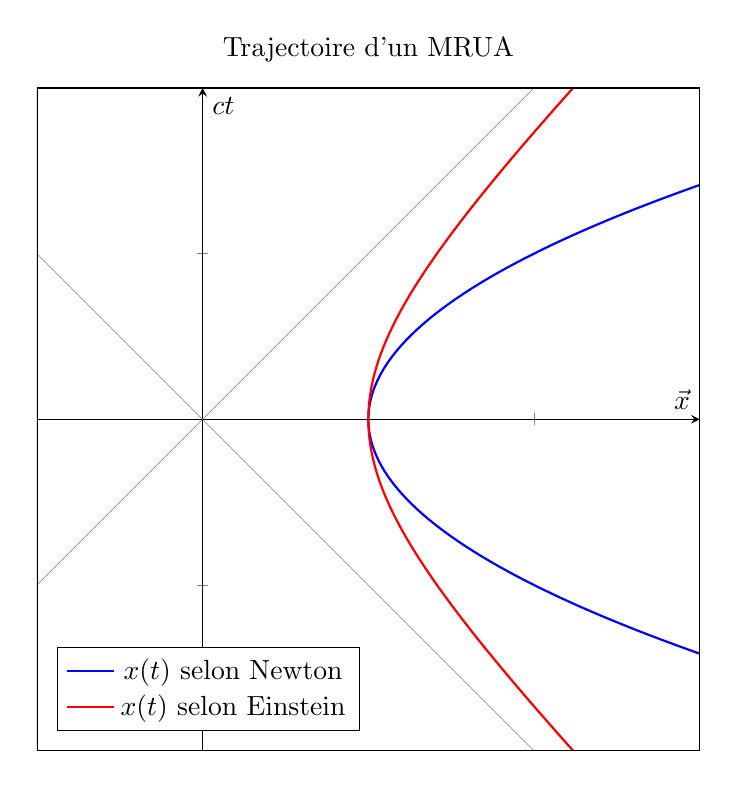
\begin{tikzpicture}
  \begin{axis}[
      samples=121, %nbre de points dans courbes parametrees
      xmin=-1,
      xmax=3,
      ymin=-2,
      ymax=2,
      width=10cm, %taille de la figure
      height=10cm,
      disabledatascaling,
      %grid=both, %afficher la grille
      %font=\footnotesize, %taille de la police par defaut
      %grid style={line width=.1pt, draw=red},
      %major grid style={line width=.2pt,draw=gray!50},
      %minor tick num=1,
      axis lines=middle,enlargelimits=0.0, %rendre le plot un rien plus grand
      %execute at begin axis={
      execute at end axis={ %cadre autour
        \draw[thick] (rel axis cs:0,0) -- (rel axis cs:1,0) -- (rel axis cs:1,1) -- (rel axis cs:0,1) --cycle;},
      xticklabels={}, %masquer les nombres en x
      yticklabels={},
      xtick={-10,-9,...,10},
      ytick={-10,-9,...,10},
      ylabel={$ct$},
      xlabel={$\vec{x}$},
      title={Trajectoire d'un MRUA},
      legend pos=south west,
    ]

    \addplot [thick, blue, domain=-1.9:1.9] ({x^2+1}, {x});
    \addlegendentry{$x(t)$ selon Newton}
    \addplot [thick, red, domain=-1.9:1.9] ({cosh(x)}, {sinh(x)});
    \addlegendentry{$x(t)$ selon Einstein}

    \addplot[help lines] expression {x};
    \addplot[help lines] expression {-x};
  \end{axis}
\end{tikzpicture}

				\caption{Position sous acceleration constante}
				\label{parabole-hyperbole}
		\end{figure}

\subsection{Le 4-vecteur force}

	\subsubsection{Définition}

		Définissons le 4-vecteur force $F^\mu_{ext}$ par extension de la seconde loi de Newton $\Vec{F} = m\cdot \Vec{a}$. Ce quadrivecteur peut également s'exprimer en utilisant le quadrivecteur <<énergie-impulsion>>:
		\begin{equation}
			\boxed{
				F^\mu_{ext} \eq
				m \cdot \omega^\mu \eq
				\dfrac{dp^\mu}{d\tau}
			}
		\end{equation}
		En travaillant composante par composante et en se rappelant que $u^0 = \dfrac{dx^0}{d\tau} = c \dfrac{dt}{d\tau} \; \Leftrightarrow \; \dfrac{dt}{d\tau} = \dfrac{u^0}{c} $, on retrouve les équations:
		\begin{align}
			\left\{
			\begin{array}{ll}
				F^0   \eq  \dfrac{d\Vec{p}}{d\tau}
				\eq \dfrac{1}{c} \dfrac{dE}{d\tau}
				\eq \dfrac{u^0}{c}\dfrac{d(E/c)}{dt}
				\eq \dfrac{u^0}{c}\dfrac{\textrm{puissance}}{c}
			\\[7pt]
				\Vec{F}  \eqq   \dfrac{d\Vec{p}}{d\tau}
				\eqq    \dfrac{u^0}{c} \dfrac{d\Vec{p}}{dt}
			\end{array}
			\right.
		\end{align}

	\subsubsection{Force et potentiel}

		Selon la théorie de Newton, la force dérive d'un potentiel: $\Vec{F}_{Newton} = -m \cdot \Vec{\nabla}V$. Il est cependant possible de montrer que $F^\mu$ ne dérive pas d'un potentiel. Pour démontrer cela, supposons que $F^\mu$ dérive d'un potentiel scalaire:
		\[
			F^\mu     \; \propto \;    \p ^\mu V    \eq    \dfrac{\p V}{\p x^\mu}
		\]
		En multipliant chacun des deux côtés de l'équation par $u^\mu$ et en se rappelant que la force est égale à la masse fois l'accélération, on obtient:
		\[
			(m \cdot \omega^\mu) \cdot u_\mu   \propto   \dfrac{\p V}{\p x^\mu} \cdot \dfrac{dx^\mu}{d\tau}
		\]
		On sait cependant que $\omega^\mu u_\mu \eq 0$:
		\[
			0    \; \propto \;  \dfrac{\p V}{\p \tau}
		\]
		Or, $ds = c \cdot d\tau$. Par conséquent:
		\[
			0    \; \propto \;  c \cdot \dfrac{dV}{ds}
		\]
		Cela voudrait dire que la particule parcourant un chemin dans un potentiel ne ressentirait aucune force, ce qui est évidemment impossible. Par conséquent, la force ne peut dériver d'un potentiel scalaire...ce qui pose problème car c'est comme ça que sont définies la force de gravitation et la force coulombienne. Heureusement, ce n'est en fait pas la force qui ne peut pas dériver d'un potentiel scalaire, mais le quadrivecteur force.

		Pour illustrer cela, prenons l'exemple d'une particule chargée décrite par le quadrivecteur $F^\mu_c$, E représentant bien l'énergie et l'indice c insistant sur le fait qu'on parle d'une force coulombienne:
		\begin{equation}
			F^\mu_c \eq
			(\; \dfrac{1}{c}\dfrac{dE_c}{d\tau}  \;,\;   \vec{F}_c \;)
			\overset{?}{\eq}
			(\; \dfrac{1}{c}\dfrac{dE_c}{d\tau}  \;,\;   q \cdot \vec{\nabla}V \;)
		\end{equation}
		Multiplions les deux côtés de l'équation par le quadrivecteur $u^\mu_c = \left(\; c\dfrac{dt}{d\tau}  \;,\;  \dfrac{d\vec{x}}{d\tau} \;\right) = \gamma (\; c \;,\; \vec{v} \;)$:
		\begin{align}
			F^\mu_c u_{c\mu}
			&\eq 0  \eq
				\eta_{\mu\nu} F^\mu_c u^\mu_c
				\\[7pt]
			&\Leftrightarrow \; 0 \eq
				\dfrac{dt}{d\tau} \cdot  c \cdot \dfrac{1}{c}\dfrac{dE_c}{d\tau}
				\;-\;
				\dfrac{d\vec{x}}{d\tau} \cdot q \cdot \vec{\nabla}V
				\\[7pt]
			&\Leftrightarrow \; 0 \eq
				\dfrac{dt}{d\tau} \dfrac{dE_c}{d\tau}
				\;-\;
				\left(\dfrac{dx^1}{d\tau},\dfrac{dx^2}{d\tau},\dfrac{dx^3}{d\tau}\right)
				\cdot q \cdot
				\left(\dfrac{\p}{\p x^1},\dfrac{\p}{\p x^2},\dfrac{\p}{\p x^3}\right) \cdot dV
				\\[7pt]
			&\Leftrightarrow \; 0 \eq
				\dfrac{dt}{d\tau} \dfrac{dE_c}{d\tau}
				\;-\;
				\dfrac{1}{d\tau} \cdot q \cdot dV
		\end{align}
		Par conséquent, dans la limite non-relativiste ($dt = d\tau$):
		\begin{equation}
			dE_c \eq q \cdot dV
		\end{equation}
		On retombe bien sur une équation connue : la variation d'énergie d'une particule chargée dans un potentiel est égale à la charge multipliée par la variation du potentiel (déplacement).






\subsection{Résumé}
\label{Résumé}

	Les différents quadrivecteurs utilisés sont:
	\begin{itemize}
		\item \makebox[5.3cm]{Le quadrivecteur position\hfill} \quad
			$x^\mu         \eq (\;   ct    \;,\;    \Vec{x}  \;)$
		\item \makebox[5.3cm]{Le quadrivecteur vitesse\hfill} \quad
			$u^\mu         \eq \dfrac{dx^\mu}{d\tau}$
		\item \makebox[5.3cm]{Le quadrivecteur d'onde\hfill} \quad
			$k^\mu         \eq (\;    \omega/c   \;,\;    \Vec{k}  \;)$
		\item \makebox[5.3cm]{Le quadrivecteur impulsion\hfill} \quad
			$p^\mu         \eq  m \cdot u^\mu \eq   (\;    E/c   \;,\;  \Vec{p}    \;)$
		\item \makebox[5.3cm]{Le quadrivecteur accélération\hfill} \quad
			$\omega^\mu    \eq \dfrac{du^\mu}{d\tau}   \eq  \dfrac{d^2x^\mu}{(d\tau)^2} $
		\item \makebox[5.3cm]{Le quadrivecteur force\hfill} \quad
			$F^\mu_{ext}   \eq     m \cdot \omega^\mu   \eq   \dfrac{dp^\mu}{d\tau}$
		\item \makebox[5.3cm]{Le quadrivecteur potentiel\hfill} \quad
			$A^\mu   \eq     (\;   \phi    \;,\;    \Vec{A}  \;)$
	\end{itemize}
	Les différentes relations utiles sont:
	\begin{itemize}
		\item Pour la lumière, $p^\mu \eq \hbar \cdot k^\mu$
		\item $ p^\mu \cdot p_\mu    \eq    \eta_{\mu\nu} \cdot p^\mu \cdot p^\nu    \eq   \dfrac{E^2}{c^2} - |\vec{p}|^2   \eq   m^2c^2 $
		\item $|\vec{p}|^2 = 0  \quad   \Leftrightarrow  \quad    E_0 = mc^2  $
		\item $u_\mu u^\mu \eq c^2$
		\item $\omega^\mu u_\mu \eq 0$
		\item $F_L^\mu   \eq   q/c \cdot F^{\mu \nu} u_{\nu}$  ;  $E = |\vec{p}$|c
		\item $\vec{a} \cdot \vec{b} \eq \delta_{ij}a^i b^j $
		\item $(\vec{a} \times \vec{b})_k \eq \epsilon_{ijk}a^i b^j $ \qquad $(\vec{a} \times \vec{b})_k$ \quad \textrm{représentant la composante k du vecteur} \quad $\vec{a} \times \vec{b}$
		\item
			\makebox[1.7cm]{ $\vec{a}\cdot(\vec{b}\times\vec{c})$ \hfill} \eq
				$\vec{a} \cdot \vec{d}$\\[7pt]
			\makebox[1.7cm]{\hfill} \eq
				$a_i \; d^i$\\[7pt]
			\makebox[1.7cm]{\hfill} \eq
				$a_i \;(\epsilon^{ijk}\;b_j \;c_k)$\\[7pt]
			\makebox[1.7cm]{\hfill} \eq
				$b_j \;\epsilon^{ijk}\;a_i \;c_k$\\[7pt]
			\makebox[1.7cm]{\hfill} \eq
				$b_i \;\epsilon^{jik}\;a_j\; c_k$  \qquad \quad \textrm{car} \quad $(i,j) \rightarrow (j,i)$\\[7pt]
			\makebox[1.7cm]{\hfill} \eq
				$b_i \;(-\epsilon^{ijk})\;a_j \;c_k$  \qquad \textrm{car} $\epsilon^{jik} \eq -\epsilon^{ijk}$\\[7pt]
			\makebox[1.7cm]{\hfill} \eq
				$- b_i \; \epsilon^{ijk} \;a_j \;c_k$\\[7pt]
			\makebox[1.7cm]{\hfill} \eq
				$- \vec{b} \cdot (\vec{a} \times \vec{c})$
	\end{itemize}
\newpage

\section{Électromagnétisme}
\subsection{Le 4-vecteur force de Lorentz}

		L'équation de la force de Lorentz est invariante selon les transformations de Lorentz\footnote{cfr. TP}. Cependant il s'agit d'un 3-vecteur et non d'un 4-vecteur, ce qui ne laisse pas transparaître cette invariance:
		\begin{equation}
			\dfrac{d\Vec{p}}{dt}    \eq   q \cdot (\Vec{E} + \dfrac{\Vec{v}}{c} \times \Vec{B} )
			\qquad \textrm{avec} \quad
			F^\mu  \eq  \dfrac{dp^\mu}{d\tau}   \eq   m \cdot \dfrac{du^\mu}{d\tau}
			\label{elec1}
		\end{equation}

	\subsubsection{Cas particulier}

		Prenons l'exemple d'une particule chargée se dirigeant vers un champ électrique perpendiculaire à sa direction de propagation (champ magnétique supposé nul). L'équation \eqref{elec1} devient alors
		\begin{equation}
			\dfrac{dp^x}{dt}    \eq   q \cdot E^x
			\label{elec3}
		\end{equation}
		Il est possible d'écrire une équation faisant intervenir l'accélération $a$ de la particule à partir de l'expression \eqref{elec3}
		\begin{equation}
			m a^x
				\eq
			m \dfrac{du^x}{d\tau}
				\eq
			\dfrac{dt}{d\tau}\dfrac{dp^x}{dt}
				\eq
			\dfrac{u^0}{c}\dfrac{dp^x}{dt}
				\eq
			\dfrac{u^0}{c}q\Vec{E}^x
				\quad \Leftrightarrow \quad
			a^x \eq \dfrac{q}{m}\Vec{E}^x
		\end{equation}
		Pour la troisième égalité, il a fallu utiliser:
		\[
			\boxed{
				\dfrac{dt}{d\tau} \eq \dfrac{u^0}{c} \eq \gamma
			}
		\]

	\subsubsection{En général}

		En reprenant en considération les deux champs et en se rappelant que $\dfrac{dt}{d\tau} = \dfrac{u^0}{c} = \gamma$, il est aisé de modifier la formule \eqref{elec1} de la force de Lorentz:
		\begin{align}
			m \cdot  \dfrac{du'}{d\tau}
				\eq \dfrac{q}{c}   u^0  (\Vec{E} + \dfrac{\Vec{v}}{c} \times \Vec{B} )
		\end{align}
		Il faut maintenant distribuer le terme $u^0$ dans la parenthèse. Il est alors possible de remplacer le terme multipliant $\Vec{B}$ grâce à:
		\[
			\Vec{v}    \eq     \dfrac{d\Vec{x}}{dt}     \eq
			\dfrac{c}{u^0} \dfrac{d\Vec{x}}{d\tau}
			\quad \Rightarrow \quad
			\Vec{u}   \eq   \dfrac{u^0\Vec{v}}{c}
		\]
		Par conséquent:
		\begin{equation}
			m \cdot  \dfrac{d\Vec{u}}{d\tau}
				\eq
			\dfrac{q}{c}  (u^0 \cdot \Vec{E} + \Vec{u} \times \Vec{B} )
			\label{elec4}
		\end{equation}
		L'équation \eqref{elec4} suggère:
		\begin{equation}
			m \cdot  \dfrac{du^\nu}{d\tau}
				\eq
			\dfrac{q}{c}  \cdot   u_\mu F^{\mu\nu}
				\quad \textrm{avec} \quad
			F^{\mu\nu}
				\eq
			\begin{pmatrix}
				0      &    -E^x       &     -E^y     &      -E^z\\
				E^x    &     0         &     -B^z     &       B^y\\
				E^y    &     B^z       &      0       &      -B^x\\
				E^z    &    -B^y       &      B^x     &      0   \\
			\end{pmatrix}
				\eq
			- F^{\nu\mu}
		\end{equation}

\subsection{Le 4-vecteur potentiel}

	Le 4-vecteur potentiel noté $A^\mu$ se définit comme la génération relativiste d'un champ de potentiel électromagnétique en mécanique classique. $\Vec{A}$ est le 3-vecteur potentiel potentiel magnétique et $\phi$ le potentiel scalaire électrique.
	\begin{align}
		 A^\mu \eq
		\begin{pmatrix}
			\phi\\
			\Vec{A}
		\end{pmatrix}
	\end{align}
	Comment exprimer $\Vec{E}$ et $\Vec{B}$ selon $A^\mu$? Commençons par rappeler l'expression du tenseur de Faraday $F^{\mu\nu} = \p^\mu A^\nu - \p^\nu A^\mu$. Sachant que $F^{00} = 0$, on peut développer pour $\nu = 0$ :
	\begin{align}
		F^{i0}
			&\eq \p^i A^0 - \p^0 A^i \\
			&\eq  \underbrace{-\Vec{\nabla}\phi}_{\textrm{(1)}} - \dfrac{1}{c} \dfrac{\p A^i}{\p t}\\
			&\eq E^i
	\end{align}
	Le signe $-$ de l'expression $(1)$ peut être surprenant mais reste correct : il s'agit de la transformation co/contravariante du quadrivecteur $x^\mu$ en le vecteur $x_\mu$.
	\begin{equation}
		x^\mu = \begin{pmatrix}ct\\ \Vec{x}\end{pmatrix}
			\quad \rightarrow \quad
		x_\mu = \begin{pmatrix}ct\\ -\Vec{x}\end{pmatrix}
			\qquad \Leftrightarrow \qquad
		\p_\mu f =
			\begin{pmatrix}
				\dfrac{\p}{c\p t}\\ \Vec{\nabla}
			\end{pmatrix} f
			\quad \rightarrow \quad
		\p^\mu f =
			\begin{pmatrix}
				\dfrac{\p}{c\p t}\\ -\Vec{\nabla}
			\end{pmatrix} f
	\end{equation}
	Pour ce qui est de l'expression de $\Vec{B}$, en développant les indices spatiaux uniquement (donc en lettres latines), on retombe sur $\Vec{B} = \Vec{\nabla} \times \Vec{A}$ :
	\begin{align}
		F^{ij}
			&=\;  \p^i A^j - \p^j A^i\\
			&=\;  \Vec{\nabla} \times \Vec{A}\\
			&=\;  \Vec{B}
	\end{align}
\newpage

\section{Les équations de Maxwell sous forme tensorielle}
\subsection{Introduction}

		Il est conseillé (et même nécessaire) de consulter l'annexe B avant d'attaquer cette section. Un tenseur peut être vu comme un objet dont chaque composante, sous un certain changement de coordonnées différentiable et inversible (défini comme un difféomorphisme), se transforme comme un objet $T^{a1,a2...am}_{b1,b2...bn}$ n-covariant et m-contravariant.

		L'objectif principal est d'écrire des équations tensorielle, c'est-à-dire des équation impliquant des tenseurs qui ne changent pas de forme quel que soit le système de coordonnées choisi : cartésiennes, circulaires, cylindriques, etc. (pour autant que ces coordonnées restent dans l'ensemble des changements autorisés pour garantir que l'objet est un tenseur). \\
		Partant du principe de relativité des référentiels inertiels, il est logique de demander une équivalence des lois de la physique entre tous les référentiels inertiels:
		\begin{itemize}
			\item Gravitation : il a été vu dans l'annexe B que la métrique $g_{\mu \nu}(t,\Vec{x})$ est bien un tenseur sous difféomorphisme, tandis que sa dérivée $\p_\rho g_{\mu \nu}$ ne l'est pas. La gravitation sera abordée plus en détail dans le cours de relativité générale.
			\item Électromagnétique : l'ensemble des équations de Maxwell peuvent s'exprimer (et c'est le but de cette section) à l'aide du tenseur antisymétrique de Faraday $F_{\mu \nu} = F_{\mu \nu}(\Vec{E}, \Vec{B}) = - F_{\nu \mu}$
		\end{itemize}

\subsection{Covariance de la théorie de Maxwell}

		Il est à noter que le terme \textit{covariance} est ici mal choisi : il n'a aucun rapport avec les composantes covariantes d'un vecteur. Il ferait plus de sens de parler (et c'est le choix du livre de référence) d'\textit{invariance de forme}, ce qui veut dire que la forme de l'équation tensorielle est invariante (ne change pas sous un changement de coordonnées).

	\subsubsection{Invariance de forme de l'expression tensorielle de la force de Lorentz}

		La force de Lorentz peut s'exprimer au moyen du tenseur de Faraday $F'^{\alpha \beta}$. Considérons l'équation de cette force dans un certain système de coordonnées :
		\[
			F_L'^{\alpha}  \eq  m \omega'^\alpha  \eq  q/c \cdot F'^{\alpha \beta} u'_\beta
		\]
		Il est possible de retrouver une équation de la même forme dans un autre système de coordonnées (transformation de chaque tenseur dans le nouveau système de coordonnées)  :
		\begin{align}
				\left(  \dfrac{\p x'^\alpha}{\p x^\mu} \right) F_L^\mu
			&= \;
				q/c  \cdot
				\left[ \;
					\left(  \dfrac{\p x'^\alpha}{\p x^\mu} \right)
					\left(  \dfrac{\p x'^\beta}{\p x^\nu}  \right)
					F^{\mu \nu}
				\; \right]
				\;
				\left(  \dfrac{\p x^\sigma}{\p x'^\beta} \right)
				u_{\sigma}\\[7pt]
			&= \;
				q/c \cdot
				\left[ \;
					\left(  \dfrac{\p x'^\alpha}{\p x^\mu} \right)
					F^{\mu \nu}
				\; \right]
				\;
				\left[ \;
					\left(  \dfrac{\p x'^\beta}{\p x^\nu}     \right)
					\left(  \dfrac{\p x^\sigma}{\p x'^\beta}  \right)
					u_{\sigma}
				\; \right] \\[7pt]
			&= \;
				q/c \cdot
				\left[ \;
					\left(  \dfrac{\p x'^\alpha}{\p x^\mu} \right)
					F^{\mu \nu}
				\; \right]
				\;
				\left[ \;
					\delta_\nu^{\; \sigma}
					u_{\sigma}
				\; \right]\\[7pt]
			&= \;
				q/c \cdot
				\left[ \;
					\left(  \dfrac{\p x'^\alpha}{\p x^\mu} \right)
					F^{\mu \nu}
				\; \right]
				\;
				u_{\nu}
		\end{align}
		En simplifiant la dernière différentielle des deux côtés de l'équation, on retombe bien sur une équation semblable à celle du début :
		\[
			\boxed{     F_L^\mu   \eq   q/c \cdot F^{\mu \nu} u_{\nu}     }
		\]
	\subsubsection{Obtenir la nouvelle forme vectorielle développée de la force de Lorentz}
		Prenons quelques lignes pour développer la différence entre la démarche du point (3.2) où nous cherchions une hypothétique transformation de la forme classique de Maxwell pour la rendre invariante sous les transformations de Galilée. Nous avions finalement conclu que la théorie de Maxwell n'était pas invariante sous ces transformations à cause des courants de déplacement.

		Développons maintenant la forme tensorielle de la force de Lorentz sous forme de produit matriciel. Il ne s'agit pas d'une méthode souvent utilisée mais elle permet ici de se passer de l'analyse indice par indice.

		Soient une matrice de pseudo-rotation $L^\alpha_{\;\mu}$ et le tenseur de Faraday $F_{araday}$ :

		\begin{align}
		\label{tenseurFmat}
			L^\alpha_{\;\mu}
				\eq
			\dfrac{\partial x'^\alpha}{\partial x^\mu}
				\eq
			\begin{pmatrix}
				ch & sh & 0 & 0\\
				sh & ch & 0 & 0\\
				0&0&1&0\\
				0&0&0&1\\
			\end{pmatrix}
				\qquad \textrm{et} \qquad
			F_{araday}
				\eq
			\begin{pmatrix}
				0    & -E^x & -E^y & -E^z \\
				E^x  & 0    & -B^z &  B^y \\
				E^y  & B^z  & 0    &  -B^x\\
				E^z  & -B^y & B^x  &  0   \\
			\end{pmatrix}
		\end{align}
		Dès lors la transformation du tenseur de Faraday entre deux référentiels $\mathcal{R}$ et $\mathcal{R'}$ peut s'écrire :
		\begin{equation}
			F'^{\alpha\beta} \eq L^\alpha_\mu F^{\mu\nu} L_\nu^\beta
			\label{Faraday}
		\end{equation}
		En appliquant le produit matriciel \eqref{Faraday}, la force de Lorentz peut être écrite selon ses coordonnées parallèles ou perpendiculaires au boost de Lorentz.
		\[
			\left\{
			\begin{array}{ll}
				\vec{E'_\parallel} \eq \vec{E_\parallel}
				\\
				\vec{E'_\perp} \eq \gamma (\vec{E_\perp} - \dfrac{\vec{v}}{c}
				\times \vec{B_\perp})
			\end{array}
			\right.
			\qquad \textrm{et} \qquad
			\left\{
			\begin{array}{ll}
				\vec{B'_\parallel} \eq \vec{B_\parallel}
				\\
				\vec{B'_\perp} \eq \gamma (\vec{B_\perp} + \dfrac{\vec{v}}{c}
				\times \vec{E_\perp})
			\end{array}
			\right.
		\]
		D'emblée, il est possible d'observer une antisymétrie entre $\vec{E}$ et $\vec{B}$ : les mêmes équations sont obtenues en effectuant le changement de variable $(\vec{E},\vec{B}) \rightarrow (\vec{B},-\vec{E})$

	\subsubsection{Transformation des équations de Maxwell homogènes}

		\begin{center}
			\boxed{\boxed{
			\textrm{ \textbf{Homogène} = indépendante du milieu (au sens charges et courants)}}}
		\end{center}
		Pour pouvoir écrire les équations de Maxwell homogènes sous forme tensorielle, commençons par réécrire les deuxième et troisième équations de Maxwell dans le vide de trois manières équivalentes\footnote{Rappelons que :$\vec{\nabla} \times (\vec{\nabla} \cdot \vec{v}) = 0$ et $\vec{\nabla} \times \vec{\nabla}C = 0$ où $C$ est un champ scalaire quelconque et $\vec{v}$ un champ vectoriel quelconque.}:
		\begin{align}
			&\left\{
			\begin{array}{ll}
				\Vec{\nabla}\cdot\vec{B}\eq 0
				\\
				\Vec{\nabla}\times\vec{E}    \eq    - \dfrac{1}{c}\dfrac{\p \vec{B}}{\p t}
			\end{array}
			\right. \\[7pt]
			\Longleftrightarrow \quad &
			\left\{
			\begin{array}{ll}
				\vec{B} \eq \vec{\nabla} \times \vec{A}
				\\
				\vec{E} \eq -\vec{\nabla}\phi - \dfrac{1}{c}\dfrac{\partial \vec{A}}{\partial t}
			\end{array}
			\right. \\[7pt]
			\Longleftrightarrow \quad &\boxed{F_{[\mu\nu , \rho]} \eq \p_\rho F_{\mu\nu} + \p_\nu F_{\rho\mu} + \p_\mu F_{\nu\rho} \eq 0}
		\end{align}
		On rappelle également que le tenseur de Faraday est \textbf{antisymétrique} et peut donc se représenter comme :
		\begin{equation}
			\boxed{
				F^{\mu\nu} \eq \p^\mu A^\nu - \p^\nu A^\mu
			}
			\qquad \textrm{avec} \quad A^\mu \overset{\Delta}{\eq} (\; \phi \;,\; \Vec{A}  \;)
		\end{equation}
		Il est considéré prouvé que $F_{[\mu\nu,\rho ]} \eq            \p_\rho F_{\mu\nu} + \p_\nu F_{\rho\mu} + \p_\mu F_{\nu\rho}$ est également un tenseur sous difféomorphisme. Or, dans un système de coordonnées comme celles de Minkowski ($M^{(4)}$), on observe que:
		\begin{equation}
			\boxed{
				F_{[\mu\nu,\rho]} \eq 0
				\quad \forall \quad
				\textrm{difféomorphisme}
			}
		\end{equation}
		L'expression des équations de Maxwell homogène sous forme tensorielle est bien invariante de forme selon les transformations de Lorentz.

	\subsubsection{Dérivation des équations vectorielles de Maxwell homogène à partir de l'équation tensorielle}

		Pour vérifier l'équivalence entre les deux formes des équations homogènes de Maxwell, il faut d'abord savoir ce que vaut $F_{\mu\nu}$:
		\[
			F_{\mu\nu}
		\eq
			\eta_{\mu\alpha} F^{\alpha\beta} \eta_{\beta\nu}
		\eq
			\begin{pmatrix}
				1 &   0 \\
				0 &  -1  \\
			\end{pmatrix}
			\cdot
			\begin{pmatrix}
				F^{00} &  F^{i0} \\
				F^{j0} &  F^{ij}  \\
			\end{pmatrix}
			\cdot
			\begin{pmatrix}
				1 &   0 \\
				0 &  -1  \\
			\end{pmatrix}
		\eq
			\begin{pmatrix}
				F^{00} &  -F^{i0} \\
				-F^{j0} &  F^{ij}  \\
			\end{pmatrix}
		\]
		Par conséquent, sachant ce que vaut $F^{\mu\nu}$ par l'équation \eqref{Faraday}:
		\[
			F_{\mu\nu} \eq
			\begin{pmatrix}
				0     & E^x  & E^y  & E^z \\
				-E^x  & 0    & -B^z &  B^y \\
				-E^y  & B^z  & 0    &  -B^x\\
				-E^z  & -B^y & B^x  &  0   \\
			\end{pmatrix}
		\]
		Il faut maintenant développer l'expression $F_{[\mu\nu,\rho]} \eq 0$ pour diverses valeurs de $\mu$, $\nu$ et $\rho$:
		\begin{itemize}

			\item Pour (1,2,3) = (x,y,z) :
			\begin{align}
				F_{[12,3]}
			&\eq
				F_{12,3} + F_{31,2} + F_{23,1} \eq 0\\[7pt]
			&\eq
				\dfrac{\p F_{12}}{\p z} + \dfrac{\p F_{31}}{\p y} + \dfrac{\p F_{23}}{\p x} \eq 0\\[7pt]
			&\eq
				-\dfrac{\p B_z}{\p z} - \dfrac{\p B_y}{\p y} - \dfrac{\p B_x}{\p x} \eq 0\\[7pt]
			&\eq
				- \vec{\nabla} \vec{B} \eq 0
			\end{align}

			\item Pour (0,1,2) = (t,x,y) :
			\begin{align}
				F_{[01,2]}
			&\eq
				F_{01,2} + F_{20,1} + F_{12,0} \eq 0\\[7pt]
			&\eq
				\dfrac{\p E_x}{\p y} - \dfrac{\p E_y}{\p x} - \dfrac{1}{c} \dfrac{\p B_z}{\p t} \eq 0\\[7pt]
			&\eq
				- (\vec{\nabla} \times \vec{E})^z - \dfrac{1}{c} \dfrac{\p B_z}{\p t} \eq 0
			\end{align}

			\item En combinant (0,1,2), (0,1,3) et (0,2,3), l'équation
			$
				\vec{\nabla} \times \vec{E} \eq - \dfrac{1}{c} \dfrac{\p \vec{B}}{\p t}
			$
			est obtenue.

		\end{itemize}
		Ainsi, les équations homogènes de Maxwell sous forme vectorielle peuvent s'obtenir à partir des équations tensorielles : les deux formes sont équivalentes.

	\subsubsection{Transformation des équations de Maxwell inhomogènes}

		Pour pouvoir écrire les équations de Maxwell inhomogènes sous forme tensorielle, commençons par réécrire les première et quatrième équations de Maxwell dans le vide:
		\[
			\left\{
			\begin{array}{ll}
				\Vec{\nabla}\cdot\vec{E}\eq \rho
				\\[7pt]
				\Vec{\nabla}\times\vec{B}  -  \dfrac{1}{c}\dfrac{\p \vec{E}}{\p t}
				\eq  \dfrac{1}{c} \vec{j}
			\end{array}
			\right.
				\quad \textrm{avec} \quad
			\left\{
			\begin{array}{ll}
				q_{tot}   \eq   \int \rho \; dV
				\\[7pt]
				\vec{j} \eq    \rho  \dfrac{d\vec{x}}{dt}
			\end{array}
			\right.
		\]
		Il est également connu \footnote{Ou plutôt supposé connu} que la quantité $
			\dfrac{1}{\sqrt{|g|}}  \;
			\left(
				\sqrt{|g|} \cdot F^{\mu \nu}
			\right)_{,\nu}
		$ , avec $|g| \overset{\Delta}{\eq} det(g_{\mu \nu})$, est un tenseur sous difféomorphisme. Dans un espace de Minkowski classique, c'est-à-dire avec la métrique $\eta_{\mu\nu}$ vue précédemment ou encore pour un espace n'étant pas soumis à la gravitation, $\sqrt{|g|} = 1$.  Il est alors possible d'égaliser ce tenseur à un autre tenseur :
		\[
				 \boxed{\p_\nu F^{\mu \nu}
				\eq
			\dfrac{1}{c} \cdot  j^\mu}
				\quad \textrm{avec} \quad
			j^\mu
				\overset{\Delta}{\eq}
			\begin{pmatrix}
				\rho c   \\
				\vec{j}\\
			\end{pmatrix}
		\]
		Cette relation est bien équivalente aux première et quatrième lois de Maxwell.
	\subsubsection{Dualité}

		En considérant les équations inhomogènes dans le vide $(\rho, \vec{j}) \rightarrow 0$, encore observer une antisymétrie entre $\vec{E}$ et $\vec{B}$ : le changement de variables $(\vec{E},\vec{B}) \rightarrow (\vec{B},-\vec{E})$ n'affecte pas les équations.

\subsection{Invariants dans l'électromagnétisme de Maxwell}

		En considérant un espace de Minkowski $M^{(4)}$ avec $g_{\mu \nu} = \eta_{\mu \nu}$, il est possible de retrouver les 4 relations suivantes :
		\begin{align*}
			&F^{\alpha \beta} \eq (\vec{E}, \vec{B})
				\qquad \overset{\textrm{dualité}}{\longleftrightarrow} \qquad
			^*F^{\alpha \beta} \eq (\vec{B}, - \vec{E})\\[7pt]
				\overset{\eta_{\alpha \beta} \eta_{\alpha \beta}}{\longleftrightarrow} \qquad
			&F_{\alpha \beta} \eq (-\vec{E}, \vec{B})
				\qquad \overset{\textrm{dualité}}{\longleftrightarrow} \qquad
			^*F_{\alpha \beta} \eq (-\vec{B}, - \vec{E})
		\end{align*}

		Ces 4 relations permettent de créer des invariants :
		\begin{itemize}
			\item   $
						F^{\mu\nu}F_{\mu\nu}
						\eqq
						2  \left(  |\vec{B}|^2 - |\vec{E}|^2  \right)
						\eqq
						 - ^* F^{\mu\nu} {}^* F_{\mu\nu}
					$
			\item  $
						F_{\mu\nu} ^* F^{\mu\nu}
						\eqq
						-4 \vec{E} \cdot \vec{B}
						\eqq
						 ^* F_{\mu\nu} F^{\mu\nu}
					 $
			\item $ det(F_{\mu\nu})  \eqq   \dfrac{1}{16} (F_{\mu\nu} ^* F^{\mu\nu})^2$
		\end{itemize}

\subsection{Galilée revisité}

		Maxwell n'a pas inventé les équations qui portent son nom. En effet, les 4 lois existaient déjà avant lui. Il ne leur manquait que le terme $\dfrac{\partial \vec{E}}{\partial t}$. Cependant son intuition physique eut de telles répercussions\footnote{Pour rappel, l'incohérence entre les lois de Maxwell et les transformations galiléennes est à la source du développement de la relativité restreinte} sur nos connaissances de la physique qu'il leur fut attribué son nom.

		Maxwell en son temps avait une vision beaucoup plus liée à la mécanique des fluides des champs électriques et magnétiques. Il savait qu'un fluide devait obéir à la condition dite de continuité qui consiste en quelques mots en une relation directe entre la variation de densité du fluide dans un volume donnée et le <<courant de sortie>> de ce même volume. Ce qui revient en somme à dire que le fluide est conservé (bilan de masse, particules, charges, etc.). Écrivons cette relation en des termes plus mathématiques :
		\begin{align}
			\dfrac{\partial \rho}{\partial t} + \vec{\nabla} \vec{j} \eq 0
		\end{align}
		Nous savons également que dans la version initiale de ces lois on pouvait écrire :
		\begin{align}
			\vec{\nabla} \times \vec{B} \eq \dfrac{\vec{j}}{c}
		\end{align}
		La divergence du vecteur densité de courant $\vec{j}$ ne pouvait donc être que 0. On obtenait donc un résultat qui défiait la logique physique : un champ ne pouvait pas sortir d'un volume donné.
		\begin{align}
			\vec{\nabla}\cdot(\vec{\nabla}\times \vec{B}) \eq 0
		\end{align}
		C'est alors que Maxwell eut l'idée d'introduire le courant de déplacement. Posons maintenant une analyse d'un point de vue galiléen sur la situation en considérant une charge et deux observateurs : un immobile par rapport à la charge et l'autre en mouvement. Par le principe d'équivalence des référentiels, les deux systèmes à la figure \eqref{refGalil} sont équivalents:
		\begin{figure}[!ht]
			\centering
			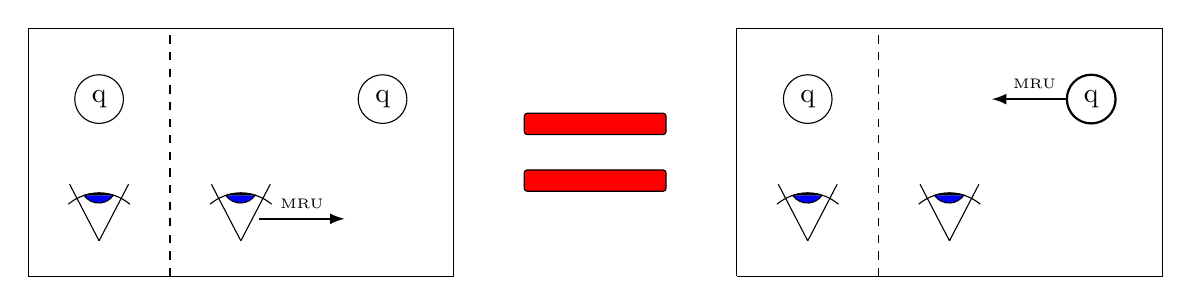
\begin{tikzpicture}[scale=0.9]
  \begin{scope}[shift={(-5,0)}]
    \draw (-1,-.5)--++(6,0)--++(0,3.5)--++(-6,0)--++(0,-3.5);
    \draw[dashed] (-1,-.5)++(2,0)--++(0,3.5);
    \node[circle, draw] at (0,2) {q};
    \eye[black]{.9}{0}{0}{90}
    \node[circle, draw] at (4,2) {q};
    \eye[black]{.9}{2}{0}{90}
    \draw[thick, -latex] (2,0)++(-55*.5+90:0.35)++(0.1,0)--++(.6,0) node[above]{\tiny{MRU}}--++(.6,0);
  \end{scope}

  \begin{scope}[shift={(5,0)}]
    \draw (-1,-.5)--++(6,0)--++(0,3.5)--++(-6,0)--++(0,-3.5);
    \draw[dashed] (-1,-.5)++(2,0)--++(0,3.5);
    \node[circle, draw] at (0,2) {q};
    \eye[black]{.9}{0}{0}{90}
    \eye[black]{.9}{2}{0}{90}
    \draw[thick, -latex] (4,2) node[circle, draw, fill=white] {q} to ++(-.8,0) node[above]{\tiny{MRU}}--++(-.6,0);
  \end{scope}

  \draw[rounded corners=1pt, fill=red] (1,0.7) rectangle ++(2,0.3);
  \draw[rounded corners=1pt, fill=red] (1,1.8) rectangle ++(2,-.3);
\end{tikzpicture}

			\caption{Deux référentiels galiléens équivalents}
			\label{refGalil}
		\end{figure}\\
		On voit donc mal sous Galilée la notion de courant de déplacement. Et pour cause, son existence provient d'une interaction entre temps et espace, ce qui est totalement impossible dans une conception galiléenne de l'espace-temps. Les équations de Maxwell inhomogènes permettent de comprendre le courant de déplacement:
		\begin{align}
			(\cRM{1})(\cRM{4}) : \quad \p_\mu F^{\mu\nu} \eq \dfrac{1}{c}j^\nu
		\quad \Leftrightarrow \quad
			\left\{
				\begin{array}{ll}
						\nu = 0
					\qquad \quad \Leftrightarrow \;
						\p_m F^{m0} \eq \rho \eq \dfrac{1}{c}j^0 \eq \vec{\nabla}\cdot \vec{E}
					\\
						\nu = 1,2,3
					\quad \Leftrightarrow \;
						\p_\mu F^{\mu n}  \eq
						\p_0 F^{0n} + \p_m F^{mn}
				\end{array}
				\right.
		\end{align}
		\begin{align}
			\p_0 F^{0\ n} \eq -\dfrac{1}{c} \dfrac{\p E^n}{\p t}   \label{galrev1}\\
			\p_m F^{m \ n} \eq \vec{\nabla}\times \vec{B}
			\label{galrev2}
		\end{align}
		Il faut maintenant justifier les équation \eqref{galrev1} et \eqref{galrev2}. Commençons par justifier l'équation \eqref{galrev1}. Nous savons que :
		\begin{align}
			\p_0 F^{0m} \eq \dfrac{1}{c} \dfrac{\p F^{0m}}{\p t} \eq
				\left\{
					\begin{array}{lll}
						\p_0 F^{01} \eq -\dfrac{1}{c} \dfrac{\p E^1}{\p t}\\
						\p_0 F^{02} \eq -\dfrac{1}{c} \dfrac{\p E^2}{\p t}\\
						\p_0 F^{03} \eq -\dfrac{1}{c} \dfrac{\p E^3}{\p t}\\
					\end{array}
				\right.
		\end{align}
		Pour ce qui est de la seconde égalité, on remarque l'indice $m$ indique bien que la dérivée ne porte que sur les dimensions spatiales et est elle-même une dérivée spatiale également. On peut donc, en partant de l'expression \eqref{tenseurFmat}, ne conserver que les indices spatiaux et réécrire :
		\begin{align}
			\p_m F^{mn}
				&= \dfrac{\p F^{mn}}{\p x^m}
				= \dfrac{\p F^{1n}}{\p x^1} + \dfrac{\p F^{2n}}{\p x^2} + \dfrac{\p F^{3n}}{\p x^3}\\
				&\Leftrightarrow
				\left\{
					\begin{array}{lll}
						\p_m F^{m1} \eq \dfrac{\p F^{11}}{\p x^1} + \dfrac{\p F^{21}}{\p x^2} + \dfrac{\p F^{31}}{\p x^3}\\
						\p_m F^{m2} \eq \dfrac{\p F^{12}}{\p x^1} + \dfrac{\p F^{22}}{\p x^2} + \dfrac{\p F^{32}}{\p x^3}\\
						\p_m F^{m3} \eq \dfrac{\p F^{13}}{\p x^1} + \dfrac{\p F^{23}}{\p x^2} + \dfrac{\p F^{33}}{\p x^3}\\
					\end{array}
				\right. \\
				&\Leftrightarrow
				\left\{
					\begin{array}{lll}
						\p_m F^{m1} \eq \dfrac{\p B^3}{\p x^2} - \dfrac{\p B^2}{\p x^3}\\
						\p_m F^{m2} \eq \dfrac{\p B^1}{\p x^3} - \dfrac{\p B^3}{\p x^1}\\
						\p_m F^{m3} \eq \dfrac{\p B^2}{\p x^1} - \dfrac{\p B^1}{\p x^2}\\
					\end{array}
				\right. \\
				&\Leftrightarrow \vec{\nabla}\times \vec{B}
		\end{align}
		Nous pouvons donc (enfin) écrire les équations de Maxwell \cRM{1} et \cRM{4} comme suit :
		\begin{equation}
			\p_\mu F^{\mu\nu} \eq \dfrac{1}{c} j^\nu
			\quad \Leftrightarrow \quad
			\left\{
					\begin{array}{ll}
						\p_\mu F^{\mu 0} \eq \rho
						\\
						\p_\mu F^{\mu m} \eq \vec{\nabla}\times \vec{B} - \dfrac{1}{c}\dfrac{\p E^m}{\p t} \eq \dfrac{1}{c} \vec{j} \qquad \textrm{cfr (10.2.3)}
					\end{array}
				\right. \\
		\end{equation}
		Dérivons de chaque côté par $\p_\nu$. On note $\p_\nu j^\nu = 0$ car la densité de charge est conservée.
		\begin{align}
			\p_\nu \p_\mu F^{\mu\nu} \eq \underbrace{\p_0 \p_\mu F^{\mu0}}_{(1)} + \underbrace{\p_m\p_\mu F^{\mu m}}_{(2)}\\
			(1) \eq \p_0 \rho
				\eq \dfrac{\p \rho}{c\p t}\\
			(2) \eq \p_m (\vec{\nabla}\times \vec{B} - \dfrac{1}{c}\dfrac{\p E^m}{\p t})
				= \p_m(\dfrac{1}{c}\vec{j})
				= \dfrac{1}{c}(\vec{\nabla}\cdot \vec{j})
				= 0 - \dfrac{1}{c} \dfrac{\p}{\p t} (\underbrace{\vec{\nabla}\cdot \vec{E}}_{(3)})\\
			(3) \eq \rho\\
			\Leftrightarrow \dfrac{1}{c}(\dfrac{\p\rho}{\p t} + \vec{\nabla}\cdot \vec{E})  = 0\\
			\Leftrightarrow \dfrac{1}{c}(\dfrac{\p\rho}{\p t} - \dfrac{\p\rho}{\p t}) = 0
		\end{align}
		On vérifie donc bien l'égalité initiale.

\subsection{Lois de transformations}

		Jusqu'ici, différentes équations de la physique se sont vues réécrites sous formes d'équations tensorielles:
		\begin{itemize}
			\item Force de Lorentz: \quad $m\omega^\mu \eq F^{\mu\nu}u_\nu$
			\item Équations de Maxwell homogènes: \quad $F_{[\mu\nu,\rho]} \eq 0$
			\item Équations de Maxwell inhomogènes: \quad
			$\dfrac{1}{\sqrt{|g|}}  \;
				\left(
					\sqrt{|g|} \cdot F^{\mu \nu}
				\right)_{,\nu}
					\eq
				\dfrac{1}{c} \cdot  j^\mu
					\quad \textrm{avec} \quad
				j^\mu
					\overset{\Delta}{\eq}
				\begin{pmatrix}
					\rho c   \\
					\vec{j}\\
				\end{pmatrix}$
		\end{itemize}
		Il est possible de montrer que cet ensemble d'équations:
		\begin{itemize}
			\item Garantit la conservation de la charge $q$ et de l'énergie $E$
			\item Découle d'une fonction scalaire : \textbf{l'action S}
		\end{itemize}

	\subsubsection{Conservation de la charge électrique}

		La charge électrique contenue dans un certain volume peut s'exprimer à l'aide de la densité de charge dans le volume considéré:
		\begin{align}
				q \eq \int \rho d^3\vec{x}
			&= \;
				\dfrac{1}{c}
				\int j^0 d^3\vec{x} \qquad \textrm{car} \quad
				j^\mu \eq (\rho c \,,\, \vec{j})
				\\[7pt]
			&= \;
				\dfrac{1}{c}
				\int_{x^0 = cst} \left[
					j^0 dx^1 dx^2 dx^3 \;+\; j^1 dx^0 dx^2 dx^3 \;+ ...
				\right]
				\qquad \textrm{là j'ai pas compris}
				\\[7pt]
			&= \;
				\dfrac{1}{c}
				\int_{x^0 = cst} j^\nu dS_\nu
		\end{align}
		Le fait que $x^0$ soit constant indique que nous considérons un temps donné : on intègre donc sur un hyperplan\footnote{même si le nom fait peur c'est juste un plan en 4D} de l'espace de Minkowski. Considérons maintenant un autre temps (donc un autre hyperplan associé à $x^0{}'$). Il est possible de montrer que l'intégrale de la densité de charge sur les deux hyperplans (donc à deux instants distincts) est la même, et ce quelle que soit l'écart entre $x^0$ et $x^0{}'$.

		Pour ce faire, intégrons la densité de charge sur le contour en vert de la figure \eqref{ContourInteg}.
		\begin{figure}[!ht]
			\centering
			\begin{tikzpicture}
  \draw[-latex] (-5,0) -- (5,0) node[above] {$x_m$};
  \draw[-latex] (0,-2) -- (0,4) node[right] {$x_0=ct$};

  \draw[-latex, gray] (3.2,1.5)--++(2,0);
  \draw[-latex, gray] (-3.2,1.5)--++(-2,0);
  \node[below right] at (0,1) {$x^0$};
  \node[above right] at (0,2) {$x^0{}'$};
  \begin{scope}[decoration={markings,mark=at position 0.65 with {\arrow[ultra thick]{latex}}}]
    \draw[  thick, black, postaction={decorate}] (-3,1)--(3,1);
    \draw[     thick, dgreen, postaction={decorate}] (3,1) arc (-90:90:0.2 and 0.5);
    \draw[  thick, black, postaction={decorate}] (3,2)--(-3,2);
    \draw[     thick, dgreen, postaction={decorate}] (-3,2) arc (90:270:0.2 and 0.5);
  \end{scope}
\end{tikzpicture}

			\caption{Contour d'intégration}
			\label{ContourInteg}
		\end{figure}\\
		L'équation \eqref{integCharge1} reliant les intégrales sur les hyperplans et les intégrales sur le contour en vert peut ainsi être directement calculée, (lat) représentant les côté latéraux:
		\begin{equation}
			\int_{x^0 = cst} j^\nu dS_\nu
		\;-\;
			\int_{x^0{}' = cst} j^\nu dS_\nu
		\eq
			\oint j^\nu dS_\nu
		\;-\;
			\int_{(lat)} j^\nu dS_\nu
		\label{integCharge1}
		\end{equation}
		En faisant tendre la largeur du contour d'intégration vers l'infini et en supposant que la distribution de charge est finie (pas de charge en $\pm \infty$), on observe que l'intégrale sur les côtés latéraux tend vers 0. Il est alors possible d'utiliser le théorème de Gauss:
		\begin{align}
			\int_{x^0 = cst} j^\nu dS_\nu
				\;-\;
			\int_{x^0{}' = cst} j^\nu dS_\nu
		&= \;
			\oint j^\nu dS_\nu\\
		&=\;
			\int c \cdot \p_\nu j^\nu \; d^4x
		\label{integCharge2}
		\end{align}
		Grâce aux équations tensorielles de Maxwell inhomogènes, on sait que $\p_\nu F^\nu = j^\mu / c$. En multipliant les deux membre de l'équation par $\p_\nu$, on obtient que $\p_\nu j^\nu = 0$. Dès lors,
		\begin{equation}
			\int_{x^0 = cst} j^\nu dS_\nu
				\;-\;
			\int_{x^0{}' = cst} j^\nu dS_\nu
		\eqq
			\int c \cdot \p_\nu j^\nu \; d^4x
		\eqq 0
		\quad \Leftrightarrow \quad
			\boxed{
			\int_{x^0 = cst} j^\nu dS_\nu \eq \int_{x^0{}' = cst} j^\nu dS_\nu
			}
		\end{equation}
		On voit donc que cette intégrale est conservée au cours du temps : sa valeur est identique quelle que soit le temps choisi. Par conséquent, l'intégrale étant équivalente à la charge comprise dans l'hyperplan, la charge est une constante:
		\begin{equation}
			q \eq cst \eq \dfrac{1}{c} \int j^\nu dS_\nu
		\end{equation}
		Les plus sagaces d'entre vous auront remarqué (ou écouté au cours) que la conservation de la charge est en réalité une conséquence de la conservation du courant : $\p_\nu j^\nu = 0$

	\subsubsection{Conservation de l'énergie-impulsion pour le champ électromagnétique}

		Cette section permet l'introduction d'un tenseur très utile en relativité générale : le tenseur énergie impulsion pour de la lumière $T^{\mu\nu}_{em}$, $em$ signifiant bien qu'il est question de radiation électromagnétique. Mathématiquement, il se définit comme:
		\begin{equation}
			T^{\mu\nu}_{em}
		\overset{\Delta}{\eq}
			\dfrac{1}{4} \eta^{\mu\nu} (F_{\alpha\beta}F^{\alpha\beta})
			\;-\;
			F^\mu_{\; \,\alpha} F^{\nu\alpha}
		\end{equation}
		Il est ainsi possible (et on va le faire) de montrer que:
		\begin{itemize}
			\item $T^{\mu\nu}$ est un tenseur symétrique : $T^{\mu\nu} = T^{\nu\mu}$\\
			Pour montrer ce résultat, il suffit de permuter tous les indices $\mu$ et $\nu$ que nous trouvons dans l'expression de $T^{\mu\nu}$. Il est également utile de se rappeler que la métrique de Minkowski est un tenseur symétrique ($\eta^{\mu\nu} = \eta^{\nu\mu}$) tandis que le tenseur de Faraday est un tenseur asymétrique ($F^{\mu\nu}=-F^{\nu\mu}$).
			\begin{align}
				T^{\nu\mu} \eq
				\dfrac{1}{4} \eta^{\nu\mu} (F_{\alpha\beta}F^{\alpha\beta})
					\,-\,
				F^\nu_{\; \,\alpha} F^{\mu\alpha}
			\eqq
				\dfrac{1}{4} \eta^{\mu\nu} (F_{\alpha\beta}F^{\alpha\beta})
					\,-\,
				(-1) F^\mu_{\; \,\alpha} (-1) F^{\nu\alpha}
			\eqq
				T^{\mu\nu}
			\end{align}

			\item La trace de $T^{\mu\nu}$ est nulle : $\eta_{\mu\nu}T^{\mu\nu} = 0$
			\begin{align}
				\eta_{\mu\nu}T^{\mu\nu}
			&=\;
				\dfrac{1}{4} \eta_{\mu\nu} \eta^{\mu\nu} (F_{\alpha\beta}F^{\alpha\beta})
					\;-\;
				\eta_{\mu\nu} F^\mu_{\; \,\alpha} F^{\nu\; \alpha}\\
			&=\;
				F_{\alpha\beta}F^{\alpha\beta}
					\;-\;
				\eta_{\mu\nu} F^\mu_{\; \,\alpha} F^{\nu\alpha}
				\qquad \textrm{car} \quad
				\eta_{\mu\nu} \eta^{\mu\nu} \eq
				\eta_{0\nu} \eta^{0\nu} +
				\eta_{m\nu} \eta^{m\nu}
				\eq 1 + 3 \cdot (-1)^2
				\eq 4\\
			&=\;
				0 \qquad \qquad \qquad \qquad \qquad \quad \; \; \,
				\textrm{car} \quad
				\eta_{\mu\nu} F^\mu_{\; \,\alpha} F^{\nu\alpha}
				\eq
			\end{align}
		\end{itemize}
		Il serait utile de pouvoir observer la conservation de ce tenseur lorsqu'on le dérive ($\eta^{\mu\nu}$ est une constante):
		\begin{align}
			\p_\nu T^{\mu\nu}
		&=\;
			\dfrac{1}{4} \eta^{\mu\nu} (F_{\alpha\beta,\nu}F^{\alpha\beta})
			\,+\,
			\dfrac{1}{4} \eta^{\mu\nu} (F_{\alpha\beta}F^{\alpha\beta}_{\;\, ,\nu})
			\,-\,
			F^\mu_{\;\,\alpha,\nu} F^{\nu\alpha}
			\,-\,
			F^\mu_{\;\,\alpha} F^{\nu\alpha}_{\;\, ,\nu}\\[7pt]
		&=\;
			\dfrac{1}{2} \eta^{\mu\nu}
			(   \underbrace{F_{\alpha\beta,\nu}}_{(1)}F^{\alpha\beta}   )
			\,-\,
			F^\mu_{\; \,\alpha,\nu} F^{\nu\alpha}
			\,-\,
			F^\mu_{\; \,\alpha} \underbrace{F^{\nu\alpha}_{\quad,\nu}}_{(2)}
			\label{EnerImp}
		\end{align}
		Or, nous savons que:
		\begin{itemize}
			\item Via les équations de Maxwell homogènes: \quad
			$
				F_{[\alpha\beta,\nu]} \eq 0
			\quad \Leftrightarrow \quad
				\p_\nu F_{\alpha\beta} \eq - \p_\beta F_{\nu\alpha} - \p_\alpha F_{\beta\nu}
			$
			\item Équations de Maxwell inhomogènes: \quad
			$F^{\nu\alpha}_{\quad ,\nu}  \eq  \dfrac{1}{c} \cdot  j^\alpha$
		\end{itemize}
		Par conséquent, les termes $(1)$ et $(2)$ peuvent être remplacés dans l'équation \eqref{EnerImp}. Les différents développements ci-dessous rappellent que $F^{\mu\nu} = - F^{\nu\mu}$ et que, même si les indices ne sont pas les mêmes, des sommes peuvent être équivalentes (de \eqref{1045} à \eqref{1046} via le changement de variable $(\alpha,\beta) \rightarrow (\beta,\alpha)$ dans l'un des deux ) :
		\begin{align}
			\p_\nu T^{\mu\nu}
		&\eqq
			\dfrac{1}{2} \eta^{\mu\nu}
			(-\p_\beta F_{\nu\alpha} - \p_\alpha F_{\beta\nu})
			F^{\alpha\beta}
			\,-\,
			F^\mu_{\;\,\alpha,\nu} F^{\nu\alpha}
			\,-\,
			F^\mu_{\;\,\alpha}      \dfrac{j^\alpha}{c}\\[7pt]
		&\eqq
			- \dfrac{1}{2} \eta^{\mu\nu}
			(F_{\nu\alpha , \beta} F^{\alpha \beta} \;+\; F_{\textcolor{red}{\beta\nu} , \alpha} F^{\textcolor{red}{\alpha\beta}})
			\,-\,
			F^\mu_{\; \,\alpha,\nu} F^{\nu\alpha}
			\,-\,
			F^\mu_{\; \,\alpha}      \dfrac{j^\alpha}{c}\\[7pt]\label{1045}
		&\eqq
			- \dfrac{1}{2} \eta^{\mu\nu}
			(F_{\nu\alpha , \beta} F^{\alpha \beta} \;+\; F_{\textcolor{red}{\nu\beta} , \alpha} F^{\textcolor{red}{\beta\alpha}})
			\,-\,
			F^\mu_{\; \,\alpha,\nu} F^{\nu\alpha}
			\,-\,
			F^\mu_{\; \,\alpha}      \dfrac{j^\alpha}{c}\\[7pt]\label{1046}
		&\eqq
			- \eta^{\mu\nu} F_{\nu\beta , \alpha} F^{\beta\alpha}
			\,-\,
			F^\mu_{\; \,\alpha,\nu} F^{\nu\alpha}
			\,-\,
			F^\mu_{\; \,\alpha}      \dfrac{j^\alpha}{c}\\[7pt]
		&\eqq
			- F^\mu_{\;\, \beta , \alpha} F^{\beta\alpha}
			\,-\,
			F^\mu_{\; \,\alpha,\nu} F^{\textcolor{red}{\nu\alpha}}
			\,-\,
			F^{\mu\;}_{\; \,\alpha}      \dfrac{j^\alpha}{c}\\[7pt]
		&\eqq
			- F^\mu_{\;\, \beta , \alpha} F^{\beta\alpha}
			\,+\,
			F^\mu_{\; \,\alpha,\nu} F^{\textcolor{red}{\alpha\nu}}
			\,-\,
			F^\mu_{\; \,\alpha}      \dfrac{j^\alpha}{c}\\[7pt]
		\p_\nu T^{\mu\nu} &\eqq
			- \dfrac{1}{c} F^{\mu\nu}j_\nu
			\label{tenseurEI}\\[7pt]
		&\eqq
			0 \qquad \textrm{en l'absence de charge:} \quad j_\nu=0
		\end{align}
		En changeant l'expression \eqref{tenseurEI} :
		\begin{align}
			0
		&= \;
			\p_\nu T^{\mu\nu} \;+\;
			\dfrac{1}{c} F^{\mu\nu}j_\nu\\[7pt]
		&= \;
			\p_\nu T^{\mu\nu} \;+\;
			\dfrac{\rho_0}{c} m F^{\mu\nu}u_\nu
			\qquad \textrm{via} \quad  j_\nu = \rho_0 u_\nu
			\\[7pt]
		&= \;
			\p_\nu T^{\mu\nu} \;+\;
			\dfrac{\rho_0}{q} m \dfrac{du^\nu}{d\tau}
			\quad \qquad \textrm{via la force de Lorentz:} \quad
			m \dfrac{du^\nu}{d\tau}
				\eq
			\dfrac{q}{c}  \cdot    F^{\mu\nu} u^\mu
			\\[7pt]
		&= \;
			\p_\nu T^{\mu\nu} \;+\;
			\dfrac{\rho}{q} m \dfrac{du^\nu}{dt}
			\quad \; \; \qquad \textrm{via} \quad
			j^\mu \eq (\rho c , \vec{j}) \eq \rho_0 u^\mu
			\quad \Leftrightarrow \quad
			\rho = \dfrac{dt}{d\tau} \rho_0
			\label{Manip}
		\end{align}
		En effectuant l'intégrale de l'expression \eqref{Manip} sur une volume de l'espace de Minkowski (donc sur $d^4x = dtd^3x$) et en effectuant le théorème de Gauss, l'expression \eqref{Manip2} est obtenue:
		\begin{align}
			cst^\mu
		&= \;
			\int \p_\nu T^{\mu\nu} d^4x
			\;+\;
			\int \dfrac{\rho}{q} m \dfrac{du^\nu}{dt} d^4x\\[7pt]
		&= \;
			\dfrac{1}{c} \int \p_\nu T^{\mu\nu} dS_\nu
			\;+\;
			m \cdot
			\dfrac{1}{q} \int \rho \,d^3x
			\cdot
			\int \dfrac{du^\nu}{dt}  dt \\[7pt]
		&= \;
			p^\mu_{em} \;+\; p^\mu_{particule}
		\label{Manip2}
		\end{align}
		Comme l'intégrale de droite a les unités d'une quantité de mouvement, l'intégrale de gauche doit nécessairement l'avoir aussi. Par conséquent, on définit l'intégrale de gauche comme la quantité de mouvement d'une onde lumineuse:
		\begin{equation}
			\boxed{
				p^\mu_{em} \eq \dfrac{1}{c} \int \p_\nu T^{\mu\nu} dS_\nu
			}
		\end{equation}
		En l'absence de charge, le membre de gauche de l'expression \eqref{Manip2} est nul et la quantité $p^\mu_{em}$ est conservée.

\newpage

\appendix

\section{Conversion énergie-impulsion} \label{AN1}
	Il sera ici abordé plusieurs exemples de conversion de l'énergie d'un système en se basant sur le vecteur $p^\mu$.

	\subsection{La désintégration}

		Considérons la désintégration d'un pion $\pi_0$ initialement au repos en deux photons:
		\[
			\pi_0 \quad \longrightarrow \quad \gamma + \gamma
		\]
		Il y a deux façons de caractériser ce phénomène: une méthode algébrique et une méthode géométrique:
		\begin{itemize}
			\item \textbf{Méthode algébrique}\\
			On sait que l'énergie et la quantité de mouvement sur chaque axe sont conservées. Par conséquent, avec les indices $i$ et $f$ dénotant les états initiaux et finaux:
			\begin{equation}
				\sum_i p^\mu_i   \eq   \sum_f p^\mu_f
				\label{consP}
			\end{equation}
			Il suffit ainsi d'écrire les différents quadrivecteurs d'impulsion et de décrire l'équation liée à chaque composante pour avoir le résultat final:
			\begin{equation}
				\left\{
					\begin{array}{lll}
						p^\mu_\pi  \quad \eq
						( m_\pi c       \;,\;  \Vec{0} )
						\\
						p^\mu_{\gamma1} \quad  \eq
						( |\Vec{p_1}|    \;,\;  \Vec{p_1} )
						\\
						p^\mu_{\gamma2} \quad  \eq
						( |\Vec{p_2}|    \;,\;  \Vec{p_2} )
					\end{array}
				\right.
				\quad \Rightarrow \quad
				\left\{
					\begin{array}{ll}
						\Vec{p_1} \eq - \Vec{p_2}
						\\
						m_\pi c \eq |\Vec{p_1}| + |\Vec{p_2}|
					\end{array}
				\right.
				\quad \Rightarrow \quad
				\Vec{p_1} \eq - \Vec{p_2} \eq \dfrac{m_\pi c}{2}
				\label{desintegration1}
			\end{equation}
			On voit ainsi que les photons ont une quantité de mouvement égale en intensité mais dans deux directions opposées.

			\item \textbf{Méthode géométrique}\\
			Les résultats des équations \eqref{desintegration1} peuvent être obtenus directement grâce à la figure \eqref{desintegration2}.
			\begin{figure}[!ht]
				\centering
				\begin{tikzpicture}
  \draw[-latex, thick] (-3,0) -- (3,0) node[above] {$\vec{p}$};
  \draw[-latex, thick] (0,-.5) -- (0,3) node[right] {$\dfrac{E}{c}$};
  \draw[help lines] (-.5,-.5) -- (2.5,2.5) (.5,-.5) -- (-2.5,2.5);
  \draw[ultra thick, red, -latex] (0,0) -- ( 1,1) node[right] {$\gamma_1$};
  \draw[ultra thick, red, -latex] (0,0) -- (-1,1) node[left] {$\gamma_2$};
  \draw[ultra thick, dgreen, -latex] (0,0) -- (0,2)node[right] {$\pi_0$} ;
\end{tikzpicture}

				\caption{représentation du problème dans l'espace de Minkowski $(E/c,\Vec{p})$}
			\label{desintegration2}
			\end{figure}\\
			En représentant correctement les vecteurs et en utilisant la conservation de chaque composante du vecteur, il est aisé d'observer que l'addition des vecteurs finaux doit donner l'addition des vecteurs initiaux (équation \eqref{consP}). Par conséquent, la quantité de mouvement des photons doit être opposée mais égale en intensité, imposant par ailleurs (via $E=pc$) l'égalité de leur énergie. De plus, cette énergie doit être égale à la moitié de l'énergie du muon au repos.
		\end{itemize}

	\subsection{La collision élastique}

		Dans le cas de la collision de plusieurs particules comme l'effet Compton pas exemple $e^- + \gamma \; \longrightarrow \; e^- + \gamma$, il est possible d'utiliser la conservation de l'énergie et de la quantité de mouvement:
		\[
			\sum\limits_{i} p^\mu_i \eq \sum\limits_{f} p^\mu_f
		\]
		On peut ainsi écrire un système dans le cas d'un électron initialement au repos.
%AJOUTER SCHEMA EXPERIENCE DE COMPTON
		\[
			\left\{
			\begin{array}{ll}
				\vec{p_\gamma} + 0     \eq     \vec{p'_\gamma} + \vec{p'_{e^-}}
			\\
				E_\gamma + m_{e^-}c^2    \eq   E'_\gamma  + E'_{e^-}
			\end{array}
			\right.
		\]
		Il est également possible d'utiliser plusieurs formules afin de résoudre ce système et d'obtenir une formule générale:
		\begin{itemize}
			\item Supprimer toute référence à l'électron:
			$
				(\dfrac{   E_{e^-}   }{c})^2 -  |\vec{p_e^-}|^2  \eq    m_{e^-}^2c^2
			$
			\item Relier la quantité de mouvement d'un photon avec son énergie:
			$
				E_\gamma    \eq    |\vec{p_\gamma}| \cdot c
			$
			\item Introduire $\lambda$ via: $E \eq \dfrac{h \cdot c}{\lambda}$
		\end{itemize}
		En combinant toutes ces équations entre elles, on obtient la formule suivante:
		\begin{equation}
			\lambda' - \lambda   \eq    2 \cdot \lambda_{e^-} \cdot \sin^2(\theta/2)
		\end{equation}

	\subsection{La collision inélastique}

		L'équation générale d'une collision inélastique est une collision entre plusieurs particules engendrant d'autres particules:
		\[
			A_1 + A_2     \; \longrightarrow \;    A_3 + A_4 + ...
		\]
		Un bon exemple de collision inélastique est l'effet photoélectrique: $ \gamma + metal    \; \longrightarrow \;    e^- + metal \; ionise$

	\subsection{Le défaut de masse $\mu$}
		Le défaut de masse $\mu$ est très certainement le concept qui illustre le mieux la conversion masse-énergie. Lors d'une collision inélastique, une partie de l'énergie cinétique des constituants est transformée en une/plusieurs particule(s). Intuitivement, la masse apparue doit trouver son équivalence dans l'énergie transformée lors de la collision.
		\begin{align}
			\mu \eq \sum_i m_i - \sum_f m_f\\
			\boxed{
				\mu c^2 \eq \sum_f \epsilon_{k,f} \; - \;  \sum_i \epsilon_{k,i}
			}
		\end{align}

	\subsection{Application: Limite de Greisen-Zatsépine-Kouzmine}
		Lorsqu'une étoile s'effondre sous forme de supernova, elle expulse un grand nombre de protons. L'univers est à une température moyenne de $2.7K$ qui représente l'énergie disséminée par le plasma primordial au moment du Big Bang. Cette température représente un bruit de fond cosmique sous forme de photons notés $\gamma_{CMB}$. Lorsque ces photons rencontrent des protons de très haute énergie (au-delà d'un certain seuil), il se produit une réacton nucléaire qui crée un pion et au autre proton moins énergétique que le premier.
		\begin{equation}
			p \; + \gamma_{CMB} \; \longrightarrow \; p' \; + \; \pi^0 \label{decpionproton}
		\end{equation}
		Le but est de calculer ce seuil d'énergie au-delà duquel les protons vont réagir\footnote{Et donc il est très rare de détecter des photons avec une énergie supérieure à ce seuil, puisqu'ils réagissent dans l'espace profond}. Commençons par exprimer l'invariant avant et après le choc : ($P$ est la somme des quadri-impulsions des particules présentes)
		\begin{align}
			P^\mu P_{\mu \text{ avant}} \eq P^\mu P_{\mu\text{ après}} \label{initgzk}
		\end{align}
		L'idée est d'exprimer cet invariant dans deux réferentiels différents avant et après la collision. Commençons par le membre de droite (après collision donc). On se place dans le référentiel centre de masse qui est défini comme le référentiel où la somme des quantités de mouvement est nulle. On peut donc écrire :
		\begin{align*}
			P^\mu_{\text{après}} &\eq
			\begin{pmatrix}
				\dfrac{E_{tot}}{c}\\[7pt]
				\vec{0}
			\end{pmatrix}\\
			\textrm{On a donc :} \qquad \; P^\mu P_{\mu\text{ après}} &\eq \dfrac{E_{tot}^2}{c^2}\\[7pt]
			&\eq \dfrac{(E_{p'} + E_{\pi_0})^2}{c^2} \\[7pt]
			&\eq  \dfrac{E_{p'}^2 + E_{\pi_0}^2 + 2 E_{p'} E_{\pi_0}}{c^2}\\[7pt]
		\end{align*}
		Et comme $E \ge mc^2$ (vrai pour toute particule) on a:
		\begin{align}
			P^\mu P_{\mu\text{ après}} & \; \ge \; m_{p}^2 c^2 + m_{\pi_0}^2 c^2 + 2 m_{p} m_{\pi_0} c^2 \label{rhsgzk}
		\end{align}
		Pour rappel, le pion $\pi^0$ se désintégrera ensuite en deux photons. Développons maintenant le membre de gauche (avant la collision): on a deux particules, le proton $p$ et le photon $\gamma$. On se place dans le repère <<labo>>\footnote{C'est à dire le repère de l'observateur, donc la terre par exemple}.
		 \begin{align}
				p^\mu_{_p} \eq
			\begin{pmatrix}
				\dfrac{E_{p}}{c}\\[7pt]
				\vec{p}_p
			\end{pmatrix}
			\qquad \text{et} \qquad p^\mu_{_\gamma} \eq
			\begin{pmatrix}
				\dfrac{E_{\gamma}}{c}\\[7pt]
				-\dfrac{E_{\gamma}}{c}
			\end{pmatrix}
		 \end{align}
	En se rappelant que (de manière générale) $p^\mu p_\mu = m^2 c^2$, on écrit:
		 \begin{align*}
			 P^\mu P_{\mu\text{ avant}} &\eq (p_{_{p}}^{\mu} + p_{_{\gamma}}^{\mu})(p_{_{p}\mu} + p_{_{\gamma}\mu})\\[7pt]
			 &\eq \underbrace{p_{_{p}}^{\mu} p_{_{p}\mu}}_{m_p^2c^2} + \underbrace{p_{_{\gamma}}^{\mu} p_{_{\gamma}\mu}}_{0} + 2 p_{_{p}}^{\mu} p_{_{\gamma}\mu}\\[7pt]
			 &\eq m_p^2 c^2 + 2 p_{_{p}}^{\mu} p_{_{\gamma}\mu}\\[7pt]
			 P^\mu P_{\mu\text{ avant}} &\eq m_p^2 c^2 + 2 \left(\dfrac{E_\gamma E_p}{c^2} + \dfrac{E_\gamma}{c} \cdot |\vec{p_{_p}}| \right)
		 \end{align*}

	Le proton se déplaçant très rapidement, on peut faire l'approximation : $\dfrac{E_p}{c} \approx p_{_p}$, on obtient donc:
	\begin{align}
		P^\mu P_{\mu\text{ avant}} &\; \approx \; m_p^2 c^2 + 2 \left(\dfrac{E_\gamma E_p}{c^2} + \dfrac{E_\gamma E_p}{c^2} \right) \eq m_p^2c^2 + 4 \dfrac{E_p E_\gamma}{c^2}\label{lhsgzk}
	\end{align}

	En combinant les équations \ref{initgzk}, \ref{rhsgzk} et \ref{lhsgzk},  on peut écrire:
		\begin{align*}
			m_p^2c^2 + 4 \dfrac{E_p E_\gamma}{c^2} &\; \ge \; m_{p}^2 c^2 + m_{\pi_0}^2 c^2 + 2 m_{p} m_{\pi_0} c^2 \\[7pt]
			4 \dfrac{E_p E_\gamma}{c^2} &\; \ge \; m_{\pi_0}^2 c^2 + 2 m_{p} m_{\pi_0} c^2
		\end{align*}
	Et donc finalement:
		\begin{align}
			E_p \; \ge \; \dfrac{(2m_pm_\pi + m_\pi^2) c^4}{4E_\gamma}
		\end{align}
	Ce qui est l'expression de la limite GZK. Sachant que:
		\[
			\left\{
			\begin{array}{lll}
				m_p = 1\text{Gev}\\
				m_{\pi^0} \approx 0.14 \text{Gev}\\
				E_{\gamma,CMB} \approx 6*10^{-4}\text{ev}\\
			\end{array}
			\right.
		\]
		On obtient que la collision décrite par l'équation \eqref{decpionproton} n'est possible que pour $E_p \ge 10^{20}$eV. Il est donc impossible d'observer sur Terre des protons cosmiques d'une énergie supérieure à $10^{20}$eV

	\subsection{Seuil énergétique d'une collision inélastique}

		Soit deux particules $A_1$ et $A_2$ telles que la première est le projectile et la seconde la cible, elle est donc \emph{au repos} par rapport au référentiel $\mathcal{R}$.

		Nous avons déjà abordé précédemment le référentiel CM $R^*$ de la particule et son intérêt dans le cadre des collisions entre particules. Rappelons que $\boxed{P^* = 0}$ tel que $P*$ est la somme des impulsions dans le référentiel $R*$.

		Rappelons également la forme générale d'une collision élastique :
		\[
			A_1 + A_2 \longrightarrow A_3 + A_4 + A_5 + ...
		\]
		L'objectif de cette section sera  de déterminer $\epsilon_s$ l'énergie seuil à partir de laquelle la réaction est possible. Dans le référentiel $R*$, les particules émergentes peuvent être toutes \emph{simultanément} au repos on aurait donc $\vec{p_f} = 0 \forall f$. On peut donc écrire :
		\begin{align}
			\epsilon^* \; \geq \; \sum_f m_f c^2
		\end{align}
		En utilisant l'invariance, exprimons l'énergie dans le référentiel propre $\epsilon^*$ :
		\begin{align}
			\epsilon^2 - P^2c^2 \eq \epsilon^{*2} - P^{*2} c^2 \eq \epsilon^{*2}\\
			\Longleftrightarrow \quad
			\epsilon^{*2} \eq (\epsilon_1 + m_2 c^2)^2 - p_1^2 c^2 \quad \textrm{car}\quad  p_2 = 0\\
			\Longleftrightarrow \quad
			(\epsilon_1 + m_2 c^2)^2 - p_1^2 c^2 \; \geq \; \sum_f m_f c^2\\
			\Longleftrightarrow \quad
			\boxed{\epsilon_1 \; \geq \; \dfrac{(\sum_f m_f c^2)^2 - (m_1^2 + m_2^2)c^4}{2m_2c^2}}
		\end{align}

	\subsection{Conclusion et motivation à l'étude de la dynamique}

		La décomposition des muons, des pions et la réaction des protons avec le bruit cosmique sont tous abordables en première approximation grâce à la cinématique relativiste. Cependant pour tenir ce raisonnement, on cloisonne les événements dans une boîte de faible taille et on ignore les rouages réels de la collision\\
		On se contente donc d'observer les interactions faibles et fortes, celles à courte portée en ignorant les interactions électromagnétiques et gravitationnelles qui elles sont à longue distance. Pour affiner nos calculs, il est nécessaire d'intégrer dans nos raisonnements ces deux interactions. Les chapitres suivant seront consacrés à intégrer l'électromagnétisme.
\newpage

\section{Formalisme tensoriel}

L'objectif de cette section est d'introduire un formalisme dont on pourrait se passer en relativité restreinte mais qui est nécessaire en relativité générale.

\subsection{Covariance et contravariance}
\subsubsection{Introduction graphique}

Tout vecteur peut s'exprimer dans une base selon ses composantes covariantes et contravariantes. Dans une base orthogonale, ces composantes sont les mêmes et c'est pour cela que la base orthogonale est souvent utilisée : elle permet d'éviter les tenseurs.

Cependant, l'abandon de la métrique euclidienne au profit de la métrique de Minkowski implique l'utilisation d'une base non-orthogonale comme représenté à la figure \ref{mink}. Considérons un vecteur $\Vec{a}$ exprimé dans une base non-orthogonale. Ce vecteur peut s'exprimer en terme de ses composantes covariantes et des ses composantes contravariantes:
\begin{figure}[!ht]
	\centering
	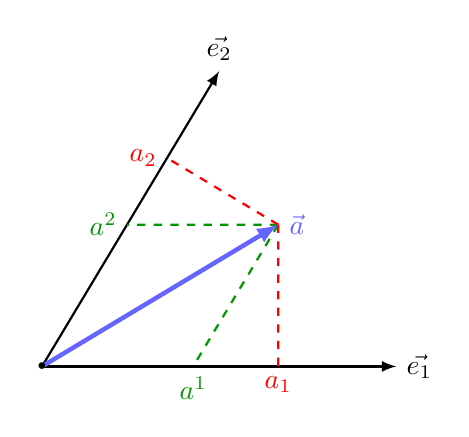
\begin{tikzpicture}[scale=1.5]
  \coordinate (a) at (2,1.2);
  \draw[-latex, thick] (0,0) -- (3,0) node[right] {$\vec{e_1}$};
  \draw[-latex, thick] (0,0) -- (1.5,2.5) node[above] {$\vec{e_2}$};
  \draw[dashed, dgreen, thick] (a) -- (1.28,0) node[below] {$a^1$};
  \draw[dashed, dgreen, thick] (a) -- (.72,1.2) node[left] {$a^2$};
  \draw[dashed, red, thick] (a) -- (2,0) node[below] {$a_1$};
  \draw[dashed, red, thick] (a) -- (9/8.5,15/8.5) node[left] {$a_2$};
  \draw[lblue, ultra thick, -latex] (0,0) -- (a) node[right] {$\vec{a}$};
  \draw (0,0) node {\tiny{$\bullet$}};
\end{tikzpicture}

	\caption{Représentation \textcolor{red}{covariante} et \textcolor{dgreen}{contravariante} d'un vecteur dans une base non-orthonormée}
\end{figure}
Les composantes contravariantes $a^i$ du vecteur $\Vec{a}$ sont les coefficients de la combinaison linéaire exprimant $\Vec{a}$ en terme de vecteur de la base:
\[\Vec{a} \eq a^i \Vec{e_i} \eq a^1 \Vec{e_1} + a^2 \Vec{e_2}\]
Les composantes covariantes $a_i$ du \textbf{même} vecteur $\Vec{a}$ sont obtenues en projetant le vecteur de façon orthogonale par rapport aux bases:
\[a_i  \eq  \Vec{a}\cdot\Vec{e_i}\]
Il est possible de passer d'un ensemble de composantes à un autre:
\[
	\Vec{a} \eq a^i \Vec{e_i}
	\quad \Leftrightarrow \quad
	\Vec{a}\cdot\Vec{e_j} \eq a^i \Vec{e_i}\cdot\Vec{e_j}
	\quad \Leftrightarrow \quad
	\boxed{    a_j \eq  a^i (\Vec{e_i} \cdot \Vec{e_j})   }
\]
On remarque donc que $\Vec{e_i} \cdot \Vec{e_j} = \p^{i}_j$ pour une base orthonormée et que donc de fait $a_j = a^i$ et que donc les composantes covariantes et contravariantes sont équivalents dans une base orthonormée.

\subsubsection{Modification de la base}

\paragraph{Base duale}  On peut avoir l'impression que les composantes contravariantes sont privilégiées aux composantes covariantes car elles multiplient les vecteurs de base. Il est possible d'inverser cette préférence en réexprimant la vecteur $\Vec{a}$ dans la base duale, càd la base dont $\Vec{e'_1}$ est orthogonal à $\Vec{e_2}$:
\begin{figure}[!ht]
	\centering
	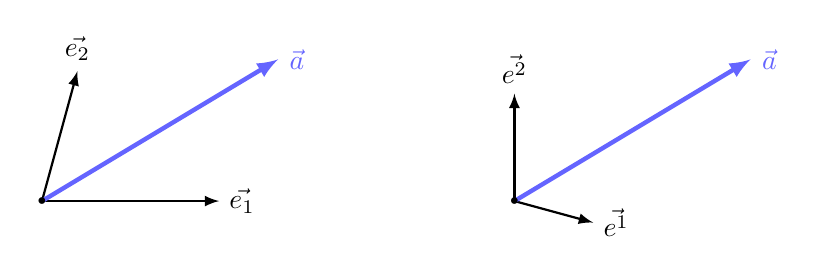
\begin{tikzpicture}[scale=1.5]
  \begin{scope}[shift={(-2,0)}]
    \draw[-latex, thick] (0,0) -- (1.5, 0) node[right] {$\vec{e_1}$};
    \draw[-latex, thick] (0,0) -- (0.3,1.1) node[above] {$\vec{e_2}$};
    \draw[lblue, ultra thick, -latex] (0,0) -- (2,1.2) node[right] {$\vec{a}$};
    \draw (0,0) node {\tiny{$\bullet$}};
  \end{scope}
  \begin{scope}[shift={( 2,0)}]
    \draw[-latex, thick] (0,0) -- (2/3, -1/5.5) node[right] {$\vec{e^1}$};
    \draw[-latex, thick] (0,0) -- (0,1/1.1) node[above] {$\vec{e^2}$};
    \draw[lblue, ultra thick, -latex] (0,0) -- (2,1.2) node[right] {$\vec{a}$};
    \draw (0,0) node {\tiny{$\bullet$}};
  \end{scope}
\end{tikzpicture}

	\caption{Une base quelconque et sa base duale}
\end{figure}
\[\Vec{a} \eq    \Vec{a^j}\Vec{e_j}  \eq    \Vec{a_i}\Vec{e^i}  \]

\paragraph{Rotation de la base} La rotation (représentée par la matrice R) de la base provoque un changement dans les composantes du vecteur $\Vec{a}$. Cependant, le vecteur $\Vec{a}$ lui-même n'a pas changé : seules ses composantes ont changé.
\begin{figure}[!ht]
	\centering
	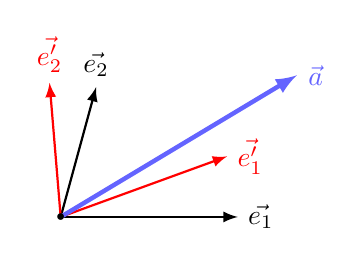
\begin{tikzpicture}[scale=1.5]
  \draw[-latex, thick] (0,0) -- (1.5, 0)  node[right] {$\vec{e_1}$};
  \draw[-latex, thick] (0,0) -- (0.3,1.1) node[above] {$\vec{e_2}$};
  \draw[-latex, thick, red, rotate=20]  (0,0) -- (1.5, 0)  node[right] {$\vec{e_1'}$};
  \draw[-latex, thick, red, rotate=20]  (0,0) -- (0.3,1.1) node[above] {$\vec{e_2'}$};
  \draw[lblue, ultra thick, -latex] (0,0) -- (2,1.2) node[right] {$\vec{a}$};
  \draw (0,0) node {\tiny{$\bullet$}};
  \centerarc[help lines, -latex] (0,0) (0.7,0,20)
  \centerarc[help lines, -latex] (0,0) (0.7,atan(1.1/0.3),atan(1.1/0.3)+20)
\end{tikzpicture}

	\caption{Une base quelconque et sa base tournée d'un certain angle}
\end{figure}
Il est donc correct d'écrire, pour les composantes contravariantes:
\[
	\Vec{a}  \eq  a^j\Vec{e_j} \eq a'^{i}\Vec{e'_i}
		\quad \textrm{avec} \quad
	\Vec{e_i'}   \eq   R^{\;j}_{i}  \Vec{e_j}
		\; \Leftrightarrow \;
	\Vec{e_j}    \eq (R^{-1})^{\; i}_{j} \Vec{e_i'}
\]
Il est alors possible de trouver une relation entre les composantes contravariantes $a^i$ et $a'^{j}$:
\[
	a^j\Vec{e_j}   \eq   a'^i  \Vec{e'_i}     \eq   a'^i  R^{\;j}_{i}  \Vec{e_j}
		\quad \Leftrightarrow \quad
	a^j   \eq   a'^i  R^{\;j}_{i}   \eq   R^{j}_{\;i} a'^i
		\quad \Leftrightarrow \quad
	\boxed{    a'^i    \eq    (R^{-1})^{i}_{\;j}      a^j  }
\]
Pour les composantes contravariantes\footnote{A noter, on parle de composantes covariantes ou contravariantes d'un vecteur (tenseur d'ordre 1), il s'agit bien de deux modes d'expressions suffisant chacun à exprimer \textbf{complètement} le vecteur. Un vecteur n'a donc pas des composantes à la fois covariantes et contravariantes.}, la matrice de changement de composantes est l'inverse de la matrice de changement de base. C'est de cet inverse que vient la dénomination \textbf{contra}variant.

En ce qui concerne les composantes covariantes, ces dernières font intervenir directement la matrice de rotation des bases et non son inverse, d'où le nom \textbf{co}variant. La formule suivante peut être démontrée de façon équivalente à ce-dessus\footnote{Et vous êtes invités à la démontrer. Vous faites moins les malins tout d'un coup.}:
\[
	\boxed{    a'_i    \eq    R^{\;j}_{i}      a_j    }
\]

\subsubsection{Conclusions sur la covariance et la contravariance}

Soit un changement de coordonnées quelconque qui est différentiable et dont l'inverse est différentiable ($\equiv$ difféomorphisme) : $x^i  \rightarrow x'^i(x)$. Il est correct d'écrire, avec $f$ une fonction quelconque:
\[
	dx'^i    \eq    (\dfrac{\p x'^i}{\p x^j}) dx^j
		\quad \Leftrightarrow \quad
	\dfrac{\p f}{\p x'^i}    \eq    (\dfrac{\p x^j}{\p x'^i}) \dfrac{\p f}{\p x^j}
		\quad \textrm{avec} \quad
	det(\dfrac{\p x'^i}{\p x^j})   \;,\;  det(\dfrac{\p x^j}{\p x'^i})
		\; \neq \; 0
\]
Cette transformation permet de définir plus précisément les notions de covariance et contravariance :
\begin{itemize}

	\item Les composantes $A^i$ d'un vecteur sont dites \textbf{contravariantes} si et seulement si, lors d'un changement de coordonnées, elles se transforment comme les différentielles d'elle-même:
	\[ \boxed{    A'^i   \eq  (\dfrac{\p x'^i}{\p x^j})  A^j   }\]

	\item Les composantes $A_i$ d'un vecteur sont dites \textbf{covariantes} si et seulement si, lors d'un changement de coordonnées, elles se transforment comme les dérivées partielles d'une fonction:
	\[ \boxed{    A'_i   \eq  (\dfrac{\p x^j}{\p x'^i})  A_j   }\]

\end{itemize}
Il est à noter qu'un tenseur $A^{a_1a_2...a_n}_{b_1b_2...b_m}$ est $n$ fois contravariant et $m$ fois covariant.

\subsection{Utilité de la notation tensorielle}

\begin{enumerate}
\item La notation tensorielle donne lieu à des invariants : $\boxed{ A'_iA'^i \eq A_iA^i}$

\item Pour savoir si un objet $A^{a_1a_2...a_n}_{b_1b_2...b_m}$ est un tenseur \textbf{sous une certaine transformation}\footnote{Il ne fait sens de dire qu'un objet est un tenseur que si la transformation est spécifiée}, il faut que chacune de ses composantes contravariante/covariante se transforme comme les composantes d'un vecteur contravariant/covariant:
\begin{itemize}
	\item $A^{ij}$ est un tenseur d'ordre 2 ssi \quad $ A'^{ij}(x') \eqq \left(\dfrac{\p x'^i}{\p x^k}\right)\; \left(\dfrac{\p x'^j}{\p x^l}\right) \; A^{kl}(x)$

	\item $A^i_{\;j}$ est un tenseur d'ordre 2 ssi \quad $A'^i_{\; \:j}(x') \eqq \left(\dfrac{\p x'^i}{\p x^k}\right) \; \left(\dfrac{\p x^l}{\p x'^j}\right) \; A^k_{\;l}(x)$

	\item $A_{ij}$ est un tenseur d'ordre 2 ssi \quad $A'_{ij}(x') \eqq \left(\dfrac{\p x^k}{\p x'^i}\right) \; \left(\dfrac{\p x^l}{\p x'^j}\right)  \; A_{kl}(x)$
\end{itemize}

\item Une équation tensorielle (ie. composée de tenseurs) garde la même forme sous un changement de coordonnées. Soit une équation tensorielle quelconque:

\begin{align*}
	A^{a_1a_2...}_{b_1b_2...} (x) &\eq  B^{a_1a_2...}_{b_1b_2...} (x) \\
	\intertext{Quand on effectue un changement de variables de $x$ vers $x'$}
	A^{a_1a_2...}_{b_1b_2...} (x) \eq  B^{a_1a_2...}_{b_1b_2...} (x)
		\quad &\xrightarrow{x \rightarrow x'} \quad
	A'^{c_1c_2...}_{d_1d_2...} (x') \eq  B'^{c_1c_2...}_{d_1d_2...} (x')
	\intertext{On multiplie les deux membres par $\pfpart{x'^{c_1}}{x^{a_1}} \pfpart{x'^{c_2}}{x^{a_2}}... \; \pfpart{x^{b_1}}{x'^{d_1}} \pfpart{x^{b_2}}{x'^{d_2}}...$}
	\underbrace{A^{a_1a_2...}_{b_1b_2...} (x) \cdot \pfpart{x'^{c_1}}{x^{a_1}}... \pfpart{x^{b_1}}{x'^{d_1}}...}_{= A'^{c_1c_2...}_{d_1d_2...} (x')}
	&\eq
	\underbrace{B^{a_1a_2...}_{b_1b_2...} (x) \cdot \pfpart{x'^{c_1}}{x^{a_1}}... \pfpart{x^{b_1}}{x'^{d_1}}...}_{= B'^{c_1c_2...}_{d_1d_2...} (x')} \\
	\intertext{Et on garde donc bien une équation de la même forme que l'équation initiale:}
	A'^{c_1c_2...}_{d_1d_2...} (x') &\eq B'^{c_1c_2...}_{d_1d_2...} (x')
\end{align*}

\item L'algèbre tensorielle est simple :
\begin{itemize}
	\item Addition : \qquad \; \; $ T^{ab} + S^{ab} = R^{ab} $
	\item Multiplication : \quad $ T^a_b \cdot S^{mp}_q = R^{amp}_{bp} $ \quad et \quad $T^a_b \cdot S^{bp}_q = R^{ap}_q$
	\item Contraction : \quad \quad $ T^{ab}_{am} = S^b_m$
\end{itemize}
\end{enumerate}

\subsection{Exemples de tenseurs}
\subsubsection{La métrique}

Reprenons tout d'abord la métrique $g_{\mu \nu}$ telle quelle. Prouvons que la métrique est un tenseur sous un changement de coordonnées quelconque :
\[
	ds^2
		\eq
	g_{\mu \nu} dx^\mu dx^\nu
		\eq
	g_{\mu \nu} \cdot \left(\dfrac{\p x^\mu}{\p x'^\alpha} \, dx'^\alpha \right) \cdot \left(\dfrac{\p x^\nu}{\p x'^\beta} \, dx'^\beta \right)
		\eq
	\left[  g_{\mu \nu}  \dfrac{\p x^\mu}{\p x'^\alpha}  \dfrac{\p x^\nu}{\p x'^\beta} \right]    \cdot   dx'^\alpha   \cdot dx'^\beta
\]
Or, $ds^2$ est un invariant:
\[
	g'_{\alpha \beta} \cdot (dx'^\alpha) \cdot (dx'^\beta)
		\eq ds^2  \eq
	\left[  g_{\mu \nu}  \dfrac{\p x^\mu}{\p x'^\alpha}  \dfrac{\p x^\nu}{\p x'^\beta} \right]    \cdot   dx'^\alpha   \cdot dx'^\beta
		\quad \Leftrightarrow \quad
	g'_{\alpha \beta}  \eq  g_{\mu \nu}  \dfrac{\p x^\mu}{\p x'^\alpha}  \dfrac{\p x^\nu}{\p x'^\beta}
\]
Ainsi, chaque composante covariante de la métrique se transforme bien comme une composante covariante d'un vecteur, et ce quel que soit la transformation. La métrique est par conséquent un tenseur sous n'importe quel changement de coordonnées.

\subsubsection{La dérivée de la métrique} \label{DerivMetr}

La dérivée de la métrique est-elle un tenseur sous certaines transformations? Nous savons déjà que
\[ g'_{\alpha \beta}  \eq  g_{\mu \nu}  \dfrac{\p x^\mu}{\p x'^\alpha}  \dfrac{\p x^\nu}{\p x'^\beta}\]
Calculons cette dérivée :
\begin{align}
		g'_{\alpha \beta, \gamma}
	& \overset{\Delta}{=} \;
		\dfrac{\p}{\p x'^\gamma} (g'_{\alpha \beta})\\[7pt]
	& =\;
		\dfrac{\p}{\p x'^\gamma}  \left[  g_{\mu \nu}  \dfrac{\p x^\mu}{\p x'^\alpha}  \dfrac{\p x^\nu}{\p x'^\beta}  \right]\\[7pt]
	& =\;
		\dfrac{\p}{\p x'^\gamma} g_{\mu \nu} \cdot
		\left(  \dfrac{\p x^\mu}{\p x'^\alpha}\right)
		\left(  \dfrac{\p x^\nu}{\p x'^\beta} \right)
	\; + \;
		g_{\mu \nu} \cdot
		\left(  \dfrac{\p}{\p x'^\gamma} \dfrac{\p x^\mu}{\p x'^\alpha} \right)
		\left(  \dfrac{\p x^\nu}{\p x'^\beta} \right)
	\; + \;
		g_{\mu \nu} \cdot
		\left(  \dfrac{\p x^\mu}{\p x'^\alpha} \right) \cdot
		\left(  \dfrac{\p}{\p x'^\gamma} \dfrac{\p x^\nu}{\p x'^\beta} \right)\\[7pt]
	& =\;
		\dfrac{\p x^\lambda }{\p x'^\gamma} g_{\mu \nu, \lambda} \cdot
		\left(  \dfrac{\p x^\mu}{\p x'^\alpha}\right)
		\left(  \dfrac{\p x^\nu}{\p x'^\beta} \right)
	 \; + \;
		g_{\mu \nu} \cdot
		\left(  \dfrac{\p^2 x^\mu}{\p x'^\gamma\p x'^\alpha} \right)
		\left(  \dfrac{\p x^\nu}{\p x'^\beta} \right)
	\; + \;
		g_{\mu \nu} \cdot
		\left(  \dfrac{\p x^\mu}{\p x'^\alpha} \right)
		\left(  \dfrac{\p^2 x^\nu}{\p x'^\gamma \p x'^\beta} \right)
\end{align}
Les deuxièmes et troisièmes termes empêchent la dérivée de la métrique d'être un tenseur sous toute transformation: ce n'est que dans le cas d'une transformation linéaire ($x \propto x'$) que les deuxièmes et troisièmes termes disparaissent.  Par conséquent, la dérivée de la métrique est un tenseur sous des transformations linéaires uniquement.

\subsubsection{Le tenseur de Faraday}

Commençons par rappeler l'expression classique de la force de Lorentz et par lui donner une nouvelle définition équivalente.

\[
	m\dfrac{dv}{dt} \eq q \cdot (\vec{E} + \dfrac{\vec{v}}{c} \times \vec{B})
\]
\[
	m\dfrac{du^\mu}{d\tau} \eq \dfrac{q}{c}F^{\mu \nu} u_\nu \eq m \omega^\mu
\]
$\omega^\mu$ représente le quadri-vecteur d'accélération relativiste. Définissons la force de Lorentz comme un objet mathématique anti-symétrique issu d'un potentiel $A$ et écrivons sa transposition dans une nouvelle base, il devient donc $F'_{\alpha \beta}$ défini comme :
\begin{equation}
	F'_{\alpha \beta}
		\overset{\Delta}{\eq}
	\p'_\alpha A'_\beta   -   \p'_\beta A'_\alpha
		\eq
	\dfrac{\p}{\p x'^\alpha} A'_\beta \; - \; \dfrac{\p}{\p x'^\beta} A'_\alpha
\end{equation}
$A'_\beta$ étant covariant il peut être réécrit comme $\dfrac{\p x^\nu}{\p x'^\beta} A_\nu$. En appliquant le même raisonnement à $A'_\alpha$ et en appliquant la dérivée, on aboutit à cette expression\footnote{Remarquez qu'à la ligne \ref{tens:3} on utilise un artifice mathématique car comme on suppose la transformation différentiable, on peut écrire $\left(\dfrac{\p x^\mu}{\p x'^\alpha}\right)   \dfrac{\p}{\p x^\mu}   \eq    \dfrac{\p}{\p x'^\alpha}$}.
\begin{align}
	F'_{\alpha \beta}
	&= \;
		\dfrac{\p}{\p x'^\alpha} A'_\beta \; - \; \dfrac{\p}{\p x'^\beta} A'_\alpha\\[7pt]
	&= \;
		\dfrac{\p}{\p x'^\alpha}
		\left(
			\dfrac{\p x^\nu}{\p x'^\beta} A_\nu
		\right)
	\quad - \quad
		\dfrac{\p}{\p x'^\beta}
		\left(
			\dfrac{\p x^\nu}{\p x'^\alpha} A_\nu
		\right) \\[7pt]
	&= \;
	\left[ \;
		\left(  \dfrac{\p x^\nu}{\p x'^\beta}   \right)
		\left(  \dfrac{\p x^\mu}{\p x'^\alpha}  \right)
		\dfrac{\p}{\p x^\mu}
		A_\nu
	+
		\dfrac{\p^2 x^\nu}{\p x'^\alpha \p x'^\beta}
		A_\nu \;
	\right]
	\; - \;
		\left[ \;
			\left(  \dfrac{\p x^\nu}{\p x'^\alpha}  \right)
			\left(  \dfrac{\p x^\mu}{\p x'^\beta}   \right)
			\dfrac{\p}{\p x^\mu}
			A_\nu
		  +
			\dfrac{\p^2 x^\nu}{\p x'^\beta \p x'^\alpha}
			A_\nu \;
		\right] \label{tens:3} \\[7pt] %ici
	&= \;
		\left(\dfrac{\p x^\nu}{\p x'^\beta}\right)
		\left(\dfrac{\p x^\mu}{\p x'^\alpha}\right)
		\dfrac{\p}{\p x^\mu}
		A_\nu
	\quad - \quad
		\left(\dfrac{\p x^\nu}{\p x'^\alpha}\right)
		\left(\dfrac{\p x^\mu}{\p x'^\beta}\right)
		\dfrac{\p}{\p x^\mu}
		A_\nu
		\label{tens}
\end{align}

Ainsi, le terme $\dfrac{\p^2 x^\nu}{\p x'^\alpha \p x'^\beta}$ est symétrique selon $\alpha$ et $\beta$ et par conséquent se simplifie avec son alter ego à l'équation \eqref{tens} de la seconde équation au contraire des deux autres termes qui ne sont pas équivalent. Les deux termes restants subissent bien deux transformations covariantes lors du changement de référentiel et $F'_{\alpha \beta}$ est donc bien un tenseur. \textbf{On constate donc bien ici que c'est le caractère antisymétrique du tenseur de Faraday qui lui garantit son statut}. Cet objet demeure un tenseur \textbf{peu importe la transformation considérée.} Il s'agit d'une exception partagée par le tenseur de la métrique. Dans un cas ordinaire, le statut de tenseur d'un objet mathématique ne peut être défini qu'en relation avec une transformation particulière.

\subsubsection{Cas de la dérivée d'un tenseur antisymétrique}

Soit $A_{\mu \nu} = -A_{\nu \mu}$ un objet mathématique antisymétrique. Écrivons maintenant la dérivée selon $x'^\gamma$ de $A'_{\alpha \beta , \gamma}$. \footnote{Ceux pour qui la dernière étape n'est pas triviale sont invités à refaire cette étape en s'aidant de la section \ref{DerivMetr}}
\begin{align}
	A'_{\alpha \beta , \gamma}
	&= \;
		\dfrac{\p}{\p x'^\gamma} (A'_{\alpha \beta})\\[7pt]
	&= \;
		\dfrac{\p}{\p x'^\gamma}
		\left[
			 A_{\mu \nu}  \dfrac{\p x^\mu}{\p x'^\alpha}  \dfrac{\p x^\nu}{\p x'^\beta}
		\right]\\[7pt]
	&= \;
		\left(\dfrac{\p x^\mu}{\p x'^\alpha}\right)
		\left(\dfrac{\p x^\nu}{\p x'^\beta}\right)
		\left(\dfrac{\p x^\rho}{\p x'^\gamma}\right)
		A_{\mu \nu , \rho}
	\quad + \quad
		\left[ \;
				\dfrac{\p^2x^\mu}{\p x'^\gamma \p x'^\alpha}
				\dfrac{\p x^\nu}{\p x'^\beta}
			\; - \;
				\dfrac{\p^2x^\mu}{\p x'^\gamma \p x'^\beta}
				\dfrac{\p x^\nu}{\p x'^\alpha}\;
		\right]
		A_{\mu \nu}
\end{align}
La dérivée d'un tenseur antisymétrique n'est donc un tenseur que si la transformation considérée est linéaire. En effet la linéarité de la transformation permet aux termes quadratiques de se simplifier et de retomber sur l'expression qui nous garantit le caractère tensoriel de l'objet.

\subsubsection{Exercice 1}

Que vaut $g'^{\alpha \beta} g'_{\alpha\beta , \gamma}$?
\begin{align*}
	g'^{\alpha \beta} g'_{\alpha\beta , \gamma}
&\eqq
		\pfpart{x'^\alpha}{x^\mu}
		\pfpart{x'^\beta }{x^\nu}
		g^{\mu \nu}
	\; \cdot \;
		\dfrac{\p }{\p x'^\gamma} \;
		\left[ \;
			\pfpart{x^\sigma  }{x'^\alpha}
			\pfpart{x^\epsilon}{x'^\beta}
			g_{\sigma \epsilon}
		\;\right]
	\\[15pt]
&\eqq
		\pfpart{x'^\alpha}{x^\mu}
		\pfpart{x'^\beta }{x^\nu}
		g^{\mu \nu}
	\; \cdot \;
		\pfpart{x^\rho }{x'^\gamma}
	\; \cdot \;
		\dfrac{\p }{\p x^\rho} \;
		\left[ \;
			\pfpart{x^\sigma  }{x'^\alpha}
			\pfpart{x^\epsilon}{x'^\beta}
			g_{\sigma \epsilon}
		\;\right]
	\\[15pt]
&\eqq
		\pfpart{x'^\alpha}{x^\mu}
		\pfpart{x'^\beta }{x^\nu}
		g^{\mu \nu}
	\; \cdot \;
		\pfpart{x^\rho }{x'^\gamma}
	\; \cdot \;
		\Big[ \;
			g_{\sigma \epsilon , \rho}
			\pfpart{x^\sigma  }{x'^\alpha}
			\pfpart{x^\epsilon}{x'^\beta}
	\\[2pt] &\hspace{2cm} \;+\;
			g_{\sigma \epsilon}
			\left(\dfrac{\p^2 x^\sigma  }{\p x^\rho \p x'^\alpha}\right)
			\pfpart{x^\epsilon}{x'^\beta}
		\;+\;
			g_{\sigma \epsilon}
			\pfpart{x^\sigma}{x'^\alpha}
			\left(\dfrac{\p^2 x^\epsilon}{\p x^\rho \p x'^\beta}\right)
		\;\Big]
	\\[15pt]
&\eqq
		\pfpart{x^\rho }   {x'^\gamma} \cdot
		\pfpart{x^\sigma}  {x^\mu}
		\pfpart{x^\epsilon}{x^\nu}
		g^{\mu\nu}
		g_{\sigma \epsilon , \rho}
	\; + \;
		\pfpart{x^\rho }{x'^\gamma} \cdot
		g^{\mu\nu}
		g_{\sigma \epsilon}
		\pfpart{x^\epsilon}{x^\nu}
		\pfpart{x'^\alpha} {x^\mu}
		\left(\dfrac{\p^2 x^\sigma  }{\p x^\rho \p x'^\alpha}\right)
	\\[2pt] &\hspace{2cm} \;+\;
		\pfpart{x^\rho }{x'^\gamma} \cdot
		g^{\mu\nu}
		g_{\sigma \epsilon}
		\pfpart{x^\sigma} {x^\mu}
		\pfpart{x'^\beta}{x^\nu}
		\left(\dfrac{\p^2 x^\epsilon}{\p x^\rho \p x'^\beta}\right)
	\\[15pt]
&\eqq
		\pfpart{x^\rho }   {x'^\gamma} \cdot
		\delta_\mu^{\;\sigma}
		\delta_\nu^{\;\epsilon}
		g^{\mu\nu}
		g_{\sigma \epsilon , \rho}
	\quad + \quad
		\pfpart{x^\rho }{x'^\gamma} \cdot
		g^{\mu\nu}
		g_{\sigma \epsilon}
		\delta_\nu^{\;\epsilon}
		\pfpart{x'^\alpha} {x^\mu}
		\left(\dfrac{\p^2 x^\sigma  }{\p x^\rho \p x'^\alpha}\right)
	\\[2pt] &\hspace{2cm} \;+\;
		\pfpart{x^\rho }{x'^\gamma} \cdot
		g^{\mu\nu}
		g_{\sigma \epsilon}
		\delta_\mu^{\;\sigma}
		\pfpart{x'^\beta}{x^\nu}
		\left(\dfrac{\p^2 x^\epsilon}{\p x^\rho \p x'^\beta}\right)
	\\[15pt]
&\eqq
		\pfpart{x^\rho }   {x'^\gamma} \cdot
		g^{\mu\nu}
		g_{\mu\nu , \rho}
	\quad + \quad
		\pfpart{x^\rho }{x'^\gamma} \cdot
		g^{\mu\nu}
		g_{\sigma \nu}
		\pfpart{x'^\alpha} {x^\mu}
		\left(\dfrac{\p^2 x^\sigma  }{\p x^\rho \p x'^\alpha}\right)
	\\[2pt] &\hspace{2cm} \;+\;
		\pfpart{x^\rho }{x'^\gamma} \cdot
		g^{\mu\nu}
		g_{\mu \epsilon}
		\pfpart{x'^\beta}{x^\nu}
		\left(\dfrac{\p^2 x^\epsilon}{\p x^\rho \p x'^\beta}\right)
	\\[15pt]
&\eqq
		\pfpart{x^\rho }   {x'^\gamma} \cdot
		g^{\mu\nu}
		g_{\mu\nu , \rho}
	\quad + \quad
		\pfpart{x^\rho }{x'^\gamma} \cdot
		\delta_\sigma^{\;\mu}
		\pfpart{x'^\alpha} {x^\mu}
		\left(\dfrac{\p^2 x^\sigma  }{\p x^\rho \p x'^\alpha}\right)
	\\[2pt] &\hspace{2cm} \;+\;
		\pfpart{x^\rho }{x'^\gamma} \cdot
		\delta_\epsilon^{\;\nu}
		\pfpart{x'^\beta}{x^\nu}
		\left(\dfrac{\p^2 x^\epsilon}{\p x^\rho \p x'^\beta}\right)
	\\[15pt]
&\eqq
		\pfpart{x^\rho }   {x'^\gamma} \cdot
		g^{\mu\nu}
		g_{\mu\nu , \rho}
	\; + \;
		\pfpart{x^\rho }{x'^\gamma} \cdot
		\Big[\;
			\pfpart{x'^\alpha}{x^\mu}
			\left(\dfrac{\p^2 x^\mu  }{\p x^\rho \p x'^\alpha}\right)
	\quad + \quad
			\pfpart{x'^\beta}{x^\nu}
			\left(\dfrac{\p^2 x^\nu  }{\p x^\rho \p x'^\beta}\right)
		\;\Big]
	\\[15pt]
&\eqq
		\pfpart{x^\rho }   {x'^\gamma} \cdot
		g^{\mu\nu}
		g_{\mu\nu , \rho}
	\quad + \quad
		2 \cdot
		\pfpart{x^\rho }{x'^\gamma} \cdot
		\pfpart{x'^\alpha}{x^\lambda}
		\left(\dfrac{\p^2 x^\lambda  }{\p x^\rho \p x'^\alpha}\right)
	\\[15pt]
&\eqq
		\pfpart{x^\rho }   {x'^\gamma} \cdot
		g^{\mu\nu}
		g_{\mu\nu , \rho}
	\quad + \quad
		2 \cdot
		\pfpart{x'^\alpha}{x^\lambda}
		\left(\dfrac{\p^2 x^\lambda  }{\p x^\rho \p x'^\alpha}\right)
	\\[15pt]
\end{align*}

\newpage

\section{Formulaire}
Cette annexe reprends ce que \textbf{nous} trouvions utile de retenir par coeur pour l'examen.

\subsection{Changement de référentiel}

	Soit $\mathcal{R}$, un référentiel au repos et $\mathcal{R'}$ un référentiel s'éloignant de $\mathcal{R}$ à vitesse constante.
	\begin{itemize}

		\item Selon Galilée :
			\begin{equation*}
				\left\{
				\begin{array}{ll}
					t' = t \\
					x' = x - v_0 \cdot t
				\end{array}
				\right.
			\end{equation*}

		\item Selon Lorentz, avec $\th(\xi) = v_0/c$ et $\ch^2 - \sh^2 = 1$ :
			\begin{equation*}
				\begin{pmatrix}
					cdt\\dx
				\end{pmatrix}
			\eq \gamma \cdot
				\begin{pmatrix}
					1 & \beta \\ \beta & 1
				\end{pmatrix}
				\begin{pmatrix}
					c dt'\\ x'
				\end{pmatrix}
			\eq
				\begin{pmatrix}
					\ch(\xi) & \sh(\xi) \\
					\sh(\xi) & \ch(\xi)
				\end{pmatrix}
				\begin{pmatrix}
					c dt'\\ x'
				\end{pmatrix}
			\end{equation*}
	\end{itemize}

\subsection{Relations utiles}

	\begin{itemize}
		\item $\vec{a} \cdot \vec{b} \eq \delta_{ij}a^i b^j \eq a_i b^i \eq a^i b_i$
		\item $(\vec{a} \times \vec{b})_k \eq \epsilon_{ijk}a^i b^j $ \qquad $(\vec{a} \times \vec{b})_k$ \quad \textrm{représentant la composante k du vecteur} \quad $\vec{a} \times \vec{b}$
		\item
			\makebox[1.7cm]{ $\vec{a}\cdot(\vec{b}\times\vec{c})$ \hfill} \eq
				$\vec{a} \cdot \vec{d}$\\[7pt]
			\makebox[1.7cm]{\hfill} \eq
				$a_i \; d^i$\\[7pt]
			\makebox[1.7cm]{\hfill} \eq
				$a_i \;(\epsilon^{ijk}\;b_j \;c_k)$\\[7pt]
			\makebox[1.7cm]{\hfill} \eq
				$b_j \;\epsilon^{ijk}\;a_i \;c_k$\\[7pt]
			\makebox[1.7cm]{\hfill} \eq
				$b_i \;\epsilon^{jik}\;a_j\; c_k$  \qquad \quad \textrm{car} \quad $(i,j) \rightarrow (j,i)$\\[7pt]
			\makebox[1.7cm]{\hfill} \eq
				$b_i \;(-\epsilon^{ijk})\;a_j \;c_k$  \qquad \textrm{car} $\epsilon^{jik} \eq -\epsilon^{ijk}$\\[7pt]
			\makebox[1.7cm]{\hfill} \eq
				$- b_i \; \epsilon^{ijk} \;a_j \;c_k$\\[7pt]
			\makebox[1.7cm]{\hfill} \eq
				$- \vec{b} \cdot (\vec{a} \times \vec{c})$
	\end{itemize}

\subsection{Additivité des vitesses}

	\begin{itemize}
		\item
		$\tanh(r_x)
		\overset{\Delta}{\eqq}
		\dfrac{v_x}{c}
		\eqq
		\dfrac{\tanh(r_x') + \tanh(r_e)}{1 + \tanh(r_x')\tanh(r_e)}$

		\item
		$v_{02}
		\eqq
		\dfrac{v_{01} \;+\; v_{12}}{1 \;+\; v_{01}v_{12} / c^2}
		$
	\end{itemize}

\subsection{Invariant de Lorentz}

	$
	ds^2
	\eqq c \cdot d\tau^2
	\eqq dx^\mu dx_\mu
	\eqq c \cdot dt^2 - |\vec{dx}|^2
	\eqq c \cdot dt'^2 - |\vec{dx'}|^2
	$

\subsection{Quadrivecteurs}

	\begin{itemize}

		\item \makebox[5.3cm]{Le quadrivecteur position\hfill} \quad
			\begin{itemize}
				\item $x^\mu  \eqq (\;   ct    \;,\;    \Vec{x}  \;)$
			\end{itemize}

		\item \makebox[5.3cm]{Le quadrivecteur vitesse\hfill} \quad
			\begin{itemize}
				\item $u^\mu \eqq \dfrac{dx^\mu}{d\tau} \eqq \gamma \cdot (c,\vec{v})$
				\item $u^\mu u_\mu \eqq \eta_{\mu\nu} u^\mu u^\nu \eqq \gamma^2 \cdot (c^2 - |\vec{v}|) \eqq c^2$
			\end{itemize}

		\item \makebox[5.3cm]{Le quadrivecteur d'onde\hfill} \quad
			\begin{itemize}
				\item $k^\mu  \eqq (\;    \omega/c   \;,\;    \Vec{k}  \;)$
				\item $k^\mu k_\mu \eqq 0 \quad \Leftrightarrow \quad \dfrac{\omega}{c} \eqq |\vec{k}|$
			\end{itemize}

		\item \makebox[5.3cm]{Le quadrivecteur impulsion\hfill} \quad
			\begin{itemize}
				\item $p^\mu \eqq \hbar \cdot k^\mu$ \quad pour la lumière
				\item $p^\mu \eqq m \cdot u^\mu \eqq \gamma \cdot (mc , m\vec{v}) \eqq   (\;    E/c   \;,\;  \Vec{p}    \;)$
				\item $ p^\mu p_\mu
				\eqq m^2 \cdot \eta_{\mu\nu} \cdot \dfrac{dx^\mu}{d\tau} \cdot \dfrac{dx^\nu}{d\tau}
				\eqq  m^2 \cdot \dfrac{c \cdot d\tau}{d\tau} \cdot \dfrac{c \cdot d\tau}{d\tau}
				\eqq m^2 c^2$
				\item $ p^\mu p_\mu
				\eqq m^2c^2
				\eqq \dfrac{E^2}{c^2} - |\vec{p}|^2
				\quad \Leftrightarrow \quad
				E^2 \eqq m^2 c^4 + |\vec{p}|^2 c^2$
			\end{itemize}

		\item \makebox[5.3cm]{Le quadrivecteur accélération\hfill} \quad
			\begin{itemize}
				\item $\omega^\mu    \eqq \dfrac{du^\mu}{d\tau}   \eqq  \dfrac{d^2x^\mu}{(d\tau)^2} $
				\item$\dfrac{dc^2}{d\tau^2} \eq 0 \eq \dfrac{d}{d\tau}(u_\mu u^\mu)
				\quad \Leftrightarrow \quad
				0 \eq \dfrac{du^\mu}{d\tau}u_\mu + \dfrac{du_\mu}{d\tau}u^\mu
				\quad \Leftrightarrow \quad
				0 \eq \omega^\mu u_\mu$
			\end{itemize}

		\item \makebox[5.3cm]{Le quadrivecteur force\hfill} \quad
			\begin{itemize}
				\item $F^\mu_{ext}   \eq     m \cdot \omega^\mu   \eq   \dfrac{dp^\mu}{d\tau}$
			\end{itemize}

		\item \makebox[5.3cm]{Le quadrivecteur potentiel\hfill} \quad
			\begin{itemize}
				\item $A^\mu   \eq     (\;   \phi    \;,\;    \Vec{A}  \;)$
			\end{itemize}

	\end{itemize}

\subsection{Taylor}

	\begin{itemize}
		\item $\dfrac{1}{1+x}
		\quad\approx\quad
		f(0) + (x-0) f'(0)
		\eqq 1 - x$

		\item $\dfrac{1}{1-x}
		\quad\approx\quad
		f(0) + (x-0) f'(0)
		\eqq 1 + x$

		\item $\dfrac{1}{\sqrt{1-x}}
		\quad\approx\quad
		f(0) + (x-0) f'(0)
		\eqq 1 - \dfrac{x}{2}$
	\end{itemize}

\subsection{Tenseurs}

	\begin{itemize}

		\item \makebox[4.3cm]{Tenseur contravariant \hfill:} \quad
			$ A'^\mu \eqq (\dfrac{\p x'^\mu}{\p x^\nu})  A^\nu$

		\item \makebox[4.3cm]{Tenseur covariant \hfill:} \quad
			$ A'_\mu \eqq (\dfrac{\p x^\nu}{\p x'^\mu})  A_\nu$

		\item \makebox[4.3cm]{Dérivée d'un tenseur \hfill:} \quad
			$ A_{\mu , \gamma}
			\eqq \p_\gamma A_\mu
			\eqq \dfrac{\p}{\p x^\gamma} A_\mu$

		\item \makebox[4.3cm]{Trace d'un tenseur \hfill:} \quad
			$ trace(A^{\mu\nu}) \eqq \eta_{\mu\nu} A^{\mu\nu}$
	\end{itemize}

\subsection{Force de Lorentz}

	\begin{itemize}
		\item Classique : $F \eqq q \cdot \left(\;   \vec{E} \;+\; \dfrac{\vec{v_{ch}}}{c} \times \vec{B} \;\right)$

		\item Relativiste : $F^\mu \eq \dfrac{q}{c}F^{\mu\nu} u_\nu$\\
		\;avec\; $F^{\mu\nu} \eqq -F^{\nu\mu} \eqq
			\begin{pmatrix}
				0     & E^x  & E^y  & E^z \\
				-E^x  & 0    & -B^z &  B^y \\
				-E^y  & B^z  & 0    &  -B^x\\
				-E^z  & -B^y & B^x  &  0   \\
			\end{pmatrix}
		\eq \p^\mu A^\nu - \p^\nu A^\mu$

		\item Dualité : le changement de variables $(E,B) \rightarrow (B,-E)$ conserve les équations.

		\item Invariants :
		\begin{itemize}
			\item \quad $F^{\mu\nu}F_{\mu\nu} \eqq 2 \cdot \left(\; |\vec{B}|^2 - |\vec{E}|^2 \;\right)$

			\item \quad $^*F^{\mu\nu}F_{\mu\nu} \eqq - 4 \cdot \vec{B} \cdot \vec{E}$
		\end{itemize}
	\end{itemize}

\subsection{Maxwell}

	\begin{equation*}
		F_{[\mu\nu , \rho]} \eq 0
		\quad \Leftrightarrow \quad
		\left\{
			\begin{array}{ll}
				\vec{\nabla} \cdot \vec{B} \eq 0 \\
				\vec{\nabla} \times \vec{E} \;+\; \dfrac{1}{c} \dfrac{\p \vec{B}}{t} \eq 0
			\end{array}
		\right.
	\end{equation*}
	\begin{equation*}
		\p_\nu T^{\mu\nu} \eq - \dfrac{1}{c} F^{\mu\nu}j_\nu
		\quad \Leftrightarrow \quad
		\left\{
			\begin{array}{ll}
				\vec{\nabla} \cdot \vec{E} \eq \dfrac{\rho}{\epsilon_0} \\[5pt]
				\vec{\nabla} \times \vec{B} \;-\; \dfrac{\p \vec{E}}{t} \eq \mu \cdot \vec{J}
			\end{array}
		\right.
	\end{equation*}

\newpage

\end{document}
